
\pagestyle{fancy} \frenchspacing
\renewcommand{\chaptermark}[1]{\markboth{#1}{}}

\renewcommand{\textfraction}{0}
\renewcommand{\floatpagefraction}{0.999}
\renewcommand{\topfraction}{0.7}
\renewcommand{\bottomfraction}{0.999}
\lfoot{}

\chapter{Grundlagen und Methoden}

\section{Etablierte Lösungsansätze}
Das Kapitel listet etablierte Lösungsansätze zur Standortermittlung einer Person auf einer Bühne und erklärt diese genauer, ebenso wie Vor- und Nachteile anhand eines Beispieles.

\subsection{Ausgangsituation des Praxisbeispiels}

Man befindet sich auf der Bühne in der Stadthalle in Ybbs. Folgende Informationen sind wichtig.
\begin{itemize}
	\item \textbf{Gerät zur Standortermittlung: } Android Smartphone
	\item \textbf{Koordinaten der Position: } TBD  
\end{itemize}

\subsection{Manuelle Steuerung}
Eine Person steht auf der Bühne der XY. Eine Möglichkeit die Steuerung der Ton- und Lichtanlagen ist diese für das Event vorher zu programmieren oder manuell während der Show zu steuern. Nun fragt sich die Person: "Wie kann ich diese Ton- und Lichtanlagen steuern?" Die Antworten folgen:

\begin{itemize}
	\item "Manuelle Steuerung der Tonanlage"
	\item "Vorprogrammierung der Lichtanlage"
\end{itemize}

An den erlangten Antworten, kann man erkennen, dass es noch keine automatisierte Lösung für das Problem gibt. Die Genauigkeit der Standortermittlung, die für die automatisierte Steuerung der Anlagen notwendig ist, kann in folgende Stufen eingeteilt werden: 

\begin{itemize}
	\item \textbf{Stufe 1: }Standort auf Bühne eingeschränkt
	\item \textbf{Stufe 2: }Standort auf Länge und Breite der Bühne eingeschränkt
	\item \textbf{Stufe 3: }Standort auf bestimmten Punkt auf der Bühne eingeschränkt
\end{itemize}

\section{Hardwareproduktion }
Im Fall von StageControl versteht man unter Hardware nicht nur Computerkomponenten, sondern auch eine eigens hergestellte Konstruktion, die das Funktionieren der Software bzw. der angesteuerten Hardwarekomponenten erst möglich macht.

\subsection{Gerüst}
So benötigen wir eine Konstruktion $\backslash$ Gerüst, welche uns ermöglicht, die Servomotoren, die Schieberegler steuern, die die Bewegung des Künstlers bzw. der Künstlerin in mechanische Bewegung übertragen, um den gewünschten Stereoeffekt erzeugen. Dies soll möglichst einfach oberhalb des benötigten Mischpults zu montieren sein.

%% /TODO: Bild einfügen

\subsection{Möglichkeiten der Hardwareproduktion}
Die Hardwareproduktion umfasst die Herstellung physischer Komponenten aus unterschiedlichen Materialien wie z. B. Kunststoff, Metall oder Holz. Diese Stoffe werden von Unternehmen eingesetzt, die sich mit der Herstellung von Hardware bzw. Prototypen befassen. Dabei gibt es verschiedene Möglichkeiten und Herangehensweisen in der Hardwareproduktion: 3D-Druck, Laser-Cutting, CNC-Fräsen und die Verwendung von Baukästen wie LEGO. Im folgenden Abschnitt wird genauer auf die Einsetzbarkeit/Verfügbarkeit, die Vor- und Nachteile zweier Produktionsarten, nämlich auf 3D-Druck und CNC-Fräsen eingegangen.

\section{3D-Druck}
\subsection{Funktionsweise}
Beim 3D-Druck handelt es sich um ein Verfahren, das Schicht für Schicht Material aufträgt, um ein dreidimensionales Objekt zu erschaffen. Dabei wird aus einer Düse das heiße Material aufgetragen, bis aus vielen Schichten das gewünschte Objekt erstellt wurde. Diese Art der Produktion wird auch als additive Fertigung bezeichnet, im Gegensatz zum CNC-Fräsen, das als subtraktive Fertigung bekannt ist.


\begin{figure}[H]
	\centering
	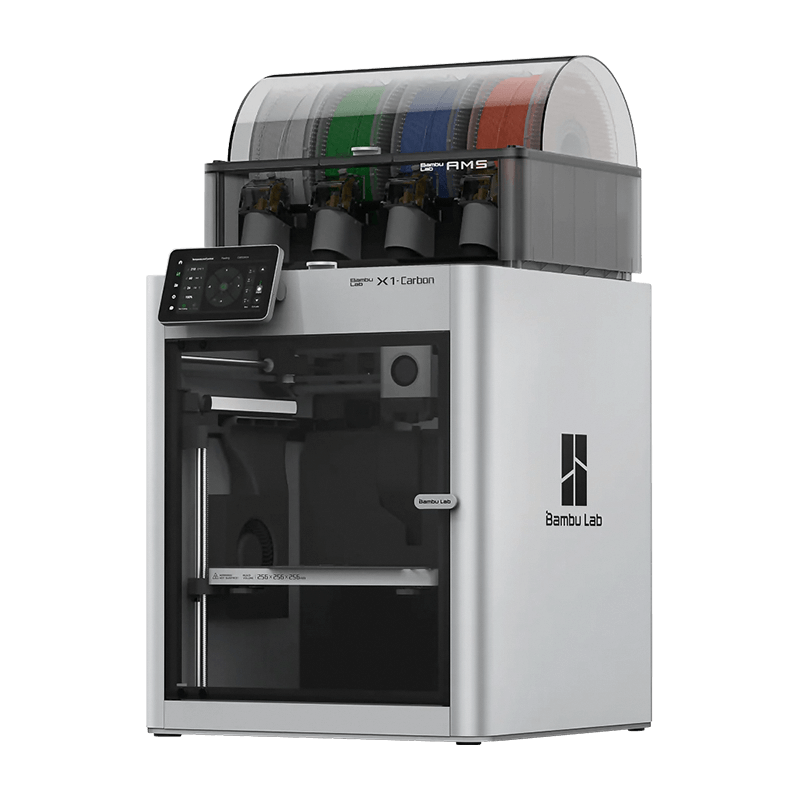
\includegraphics[width=0.5\linewidth]{images/3D-Drucker.png}
	\caption[Bambu Lab X1-Carbon 3 Pro]{Bambu Lab X1-Carbon 3 Pro}
	\label{fig:3D-Druck}
\end{figure}


\subsection{Vorteile des 3D-Drucks}
3D-Druck bietet viele Vorteile für Privatkunden und Unternehmen. Die nachfolgenden Vorteile zählen zu den wichtigsten:
\begin{itemize}
	\item Möglichkeit, komplexe Objekte relativ schnell herzustellen.
	\item Keine Vorlaufzeit nötig, d.h. keine Werkzeugproduktion erforderlich.
	\item Rapid Prototyping (\textit{deutsch „schnelle Prototypenherstellung“})
	\item Kostengünstige Produktion
	\item Herstellung individueller Objekte
\end{itemize} \parencite{3DDruckVorteile}

\subsection{Nachteile des 3D-Druck}
3D-Druck bietet aber nicht nur Vorteile, sondern hat wie alle Technologien seine Nachteile und Schwächen.
\begin{itemize}
	\item Nachbearbeitung der Konstruktionen nötig.
	\item Nicht so genau wie subtraktive Fertigungverfahren.
	\item Lange Fertigungszeiten
	\item Begrenztes Bauvolumen
\end{itemize}
\parencite{3DDruckNachteile}

\subsection{Technische Voraussetzungen}
Um den 3D-Druck technisch durchführen zu können, werden folgende Komponenten benötigt:
\begin{itemize} 
	\item 3D-Drucker
	\item Slicer
	\item CAD-Programm
	\item 3D-Druck Material (Filament)
	\item Computer
\end{itemize}
Auf den nächsten Seiten wird auf diese Punkte näher eingegangen und ein Vergleich erstellt um die Vor- und Nachteile \parencite{3ds} der genannten 3D-Drucker zu veranschaulichen. 


\subsection{Druckverfahren}

Um Hardware mittels 3D-Drucks zu erstellen, gibt es verschiedene Möglichkeiten, das Ausgangsmaterial \parencite{3ds} in die gewünschte Form zu bringen. Die gängigsten und weitverbreitesten Verfahren \parencite{kaffka} im Überblick: 

\begin{itemize}
	\item \textbf{FFF:} (Fused Filament Fabrication) oder \textbf{FDM} (Fused Deposition Modelling): Hierbei wird Kunststofffilament (\textit{eine einzelne Faser beliebig lang}) verwendet und Schicht für Schicht aufgetragen.
	\item \textbf{SLA:} Diese Technologie verwendet lichtempfindliches Kunstharz, das sich verfestigt. Wird ebenfalls Schicht für Schicht aufgetragen.
	\item \textbf{PBF:} Eine Möglichkeit, diese pulverbasierte Technologie zu nutzen, ist, das Pulver mittels Laser miteinander zu verschmelzen.  
\end{itemize}


\subsection{Werkstoffe}
3D-Drucker benötigen zum Drucken eines Objektes Material, das sie verbrauchen können, um das Objekt herzustellen. Im Rahmen dieser Diplomarbeit werden zwei Werkstoffe ganuer analysiert, nämlich Nylon und Kohlefaser.

\subsubsection{Nylon}
Nylon (\textit{techn. Polyamid}) ist ein langlebiges Material, das sich vorallem durch seine Widerstandfähigkeit gegen Hitze und mechanischen Außeneinwirkungen auszeichnet \parencite{Nylon}. Nylon gibt es in unterschiedlichen Ausführungen: als Filament, Draht oder Pulver mit unterschiedlichen Eigenschaften. 

\subsubsection{Kohlefaser}
Kohlefasern wird in Grundpolymeren wie PLA oder Nylon eingearbeitet \parencite{Kohlefasern} um eine höhere Stabilität und Resistenz zu erzeugen wie zb. Nylon verstärkt mit Kohlefasern.\\



\subsection{3D-Drucker}

\subsubsection{Vergleich der 3D-Drucker}
Wie in der Einleitung des Kapitels \textit{"Hardware im Zusammenhang mit StageControl"} beschrieben, ist eine Möglichkeit zur Herstellung der benötigten Hardware das Drucken mittels eines 3D-Druckers. Um die 3D-Drucker (\textit{Bambu Lab X1-Carbon, Ultimaker 2 Extended+, Bambu Lab A1})  \parencite{Ultimaker2ExtendedSpecification} \parencite{BambuLabA1} miteinander zu vergleichen, werden folgende Kriterien herangezogen: die Verarbeitbarkeit des Ausgangsmaterials und die Druckgeschwindigkeit bei einem Düsendurchmesser von 0,4 mm \parencite{BambuLabX1Carbon3DPrinterSpecifications}. 

Als Ausgangsmaterial wird bei allen 3D-Druckern PLA verwendet.
\begin{table} [H]
	\begin{tabular}{ |p{2.7cm} |p{4cm}|p{4cm}|p{4cm}| }
		\hline
		\textbf{Kriterien} & \textbf{Ultimaker 2 Extended+} & \textbf{Bambu Lab X1-Carbon 3 Pro} & \textbf{Bambu Lab A1} \\
		\hline
		\textbf{Material (PLA)} & Kann verarbeitet werden & Kann verarbeitet werden & Kann verarbeitet werden \\
		\hline
		\textbf{Drucktempo} & Druckt mit einer Geschwindigkeit von 16 mm\textsuperscript{3}/s & Druckt mit einer Geschwindigkeit von 32 mm\textsuperscript{3}/s & Druckt mit einer Geschwindigkeit von 18 mm\textsuperscript{3}/s \\
		\hline
		\textbf{Druckvolumen} & 223 x 223 x 205 mm & 256 x 256 x 256 mm & 256 x 256 x 256 mm \\
		\hline
		\textbf{Betriebssysteme} & MacOS, Windows, und Linux & Windows, MacOS & Windows, MacOS \\
		\hline
		\textbf{Druck-technologie} & FDM (Fused Deposition Modeling) & FDM (Fused Deposition Modeling) & FDM (Fused Deposition Modeling) \\
		\hline
		\textbf{Anschluss-möglichkeiten} & USB, SD-Karte & Wi-Fi, Ethernet, USB-C & Wi-Fi, USB, Ethernet \\
		\hline
	\end{tabular}
	\caption{Vergleich Ultimaker 2 Extended+, Bambu Lab X1-Carbon 3 Pro und Bambu Lab A1}
\end{table}



\subsection{Slicer}
\subsubsection{Was ist ein Slicer?}
Ein Slicer ist ein Stück Software, das es erst möglich macht 3D-Modelle auszudrucken, indem es einen sogenannten G-Code erstellt . G-Code ist die Programmiersprache, die von Computern verwendet wird, um mit Maschinen zu kommunizieren, wenn die Maschine Bewegungen ausführen soll. \parencite{SlicerGCode} \\



\section{CNC-Fräsen}

Ein weiterer Ansatz zur Hardware- bzw. Prototypenherstellung, der für StageControl benötigt wird, ist das CNC-Fräsen (\textit{engl. "Computerized Numerical Control"}). Diese Technologie wird vor allem in der metallverarbeitenden Industrie angewendet \parencite{CNCFraesen}, da sie äußerst genau und kostengünstig arbeitet. Zudem beschränkt sich das CNC-Fräsen nicht nur auf Metall, es kann auch bei der Bearbeitung von Kunststoffen und Holz eingesetzt werden \parencite{CNCFraesen2}. Anders als bei der 3D-Druck-Technologie handelt es sich hier nicht um ein additives, sondern um ein subtraktives Verfahren.\\  \parencite{CNCFraesen3}


\begin{figure}[H]
	\centering
	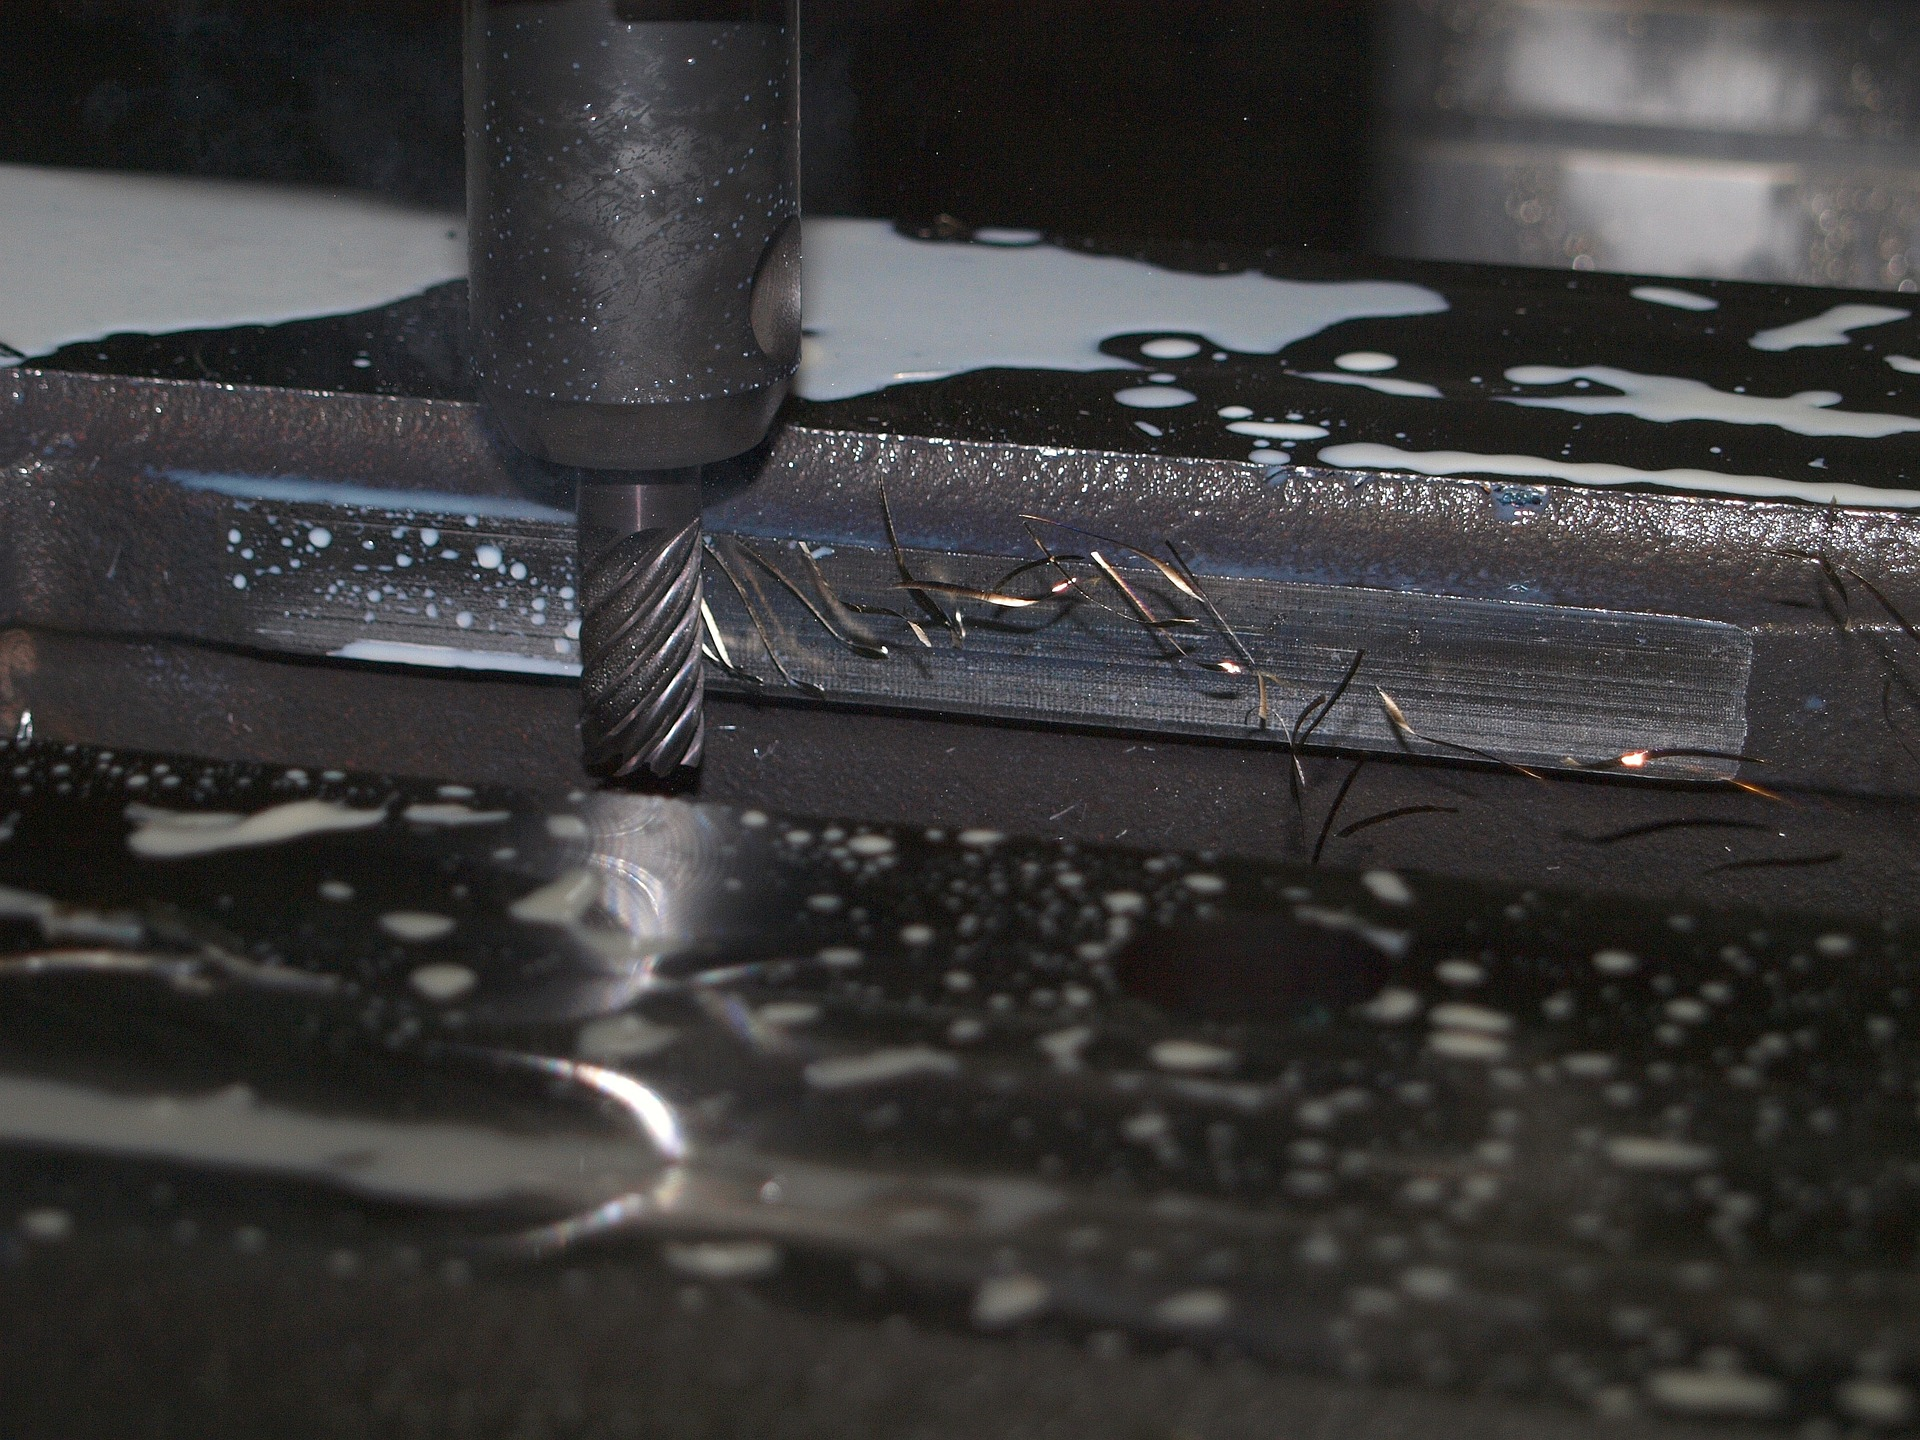
\includegraphics[width=0.6\linewidth]{images/CNC.jpg}
	\caption[CNC-Fräse]{CNC-Fräse}
	\label{fig:cnc-fraese}
\end{figure}

\subsection{Funktionsweise}
Wie bereits in der Einleitung zum CNC-Fräsen erläutert, handelt es sich um ein subtraktives Verfahren, bei dem Material entfernt wird. Das Ausgangsmaterial wird fest in die Maschine eingespannt, während sich der Fräser bewegt \parencite{CNCFraesen2}. Der Fräser trägt dann das Material ab, um die gewünschte Form herzustellen. Um besonders präzise Abrundungen zu erzeugen, wird nicht das Material, sondern der Fräskopf fixiert, während sich das Material bewegt  \parencite{CNCFraesen3}. Wie beim 3D-Druck wird hier auch G-Code als Steuerung der Maschine eingestzt. \\



\subsubsection{Einsatzmöglichkeiten}
CNC-Fräsmaschinen können vielseitig eingesetzt werden und eine Vielzahl von Objekten in unterschiedlichsten Größen und Formen herstellen  \parencite{CNCFraesen2}. Zu den typischen Anwendungsbereichen zählen unter anderem:

\begin{itemize}
	\item Maschinenteilherstellung: Komponenten von Maschinen, die nur geringe Toleranzen zulassen.
	\item Prototypen: Herstellung von ersten Modellen in geringen Stückzahlen.
\end{itemize}

Durch den Einsatz von CNC-Fräsen können menschliche Fehler und die Ausschussrate minimiert werden. Dies führt zu niedrigeren Stückkosten, was sich besonders bei der Serienfertigung bemerkbar macht.\\  \parencite{CNCFraesen3}


\subsubsection{Vorteile des CNC-Fräsens}
CNC-Fräsen bietet im Vergleich zum herkömmlichen, manuellen Fräsen einige Vorteile. Wie bei jeder manuellen Arbeit können Arbeitsunfälle passieren. Durch den Einsatz moderner CNC-Fräsen, die aus der Ferne gesteuert werden können, lassen sich solche Unfälle reduzieren \parencite{CNCFraesenVorteile}. Ein weiterer Vorteil des CNC-Fräsens ist seine gleichbleibende Genauigkeit, da die CNC-Fräse computergesteuert ist. Diese Technologie wird vor allem bei Werkstücken eingesetzt, die nur wenig Toleranz in der Genauigkeit zulassen. CNC-Fräsen arbeiten mit einer Präzision von 0,01 bis 0,03 mm. \\


\subsection{CNC gesteuerte Maschinen}
Es gibt nicht nur CNC-Fräsen oder Drehen, sondern alle Maschinen die durch CNC (\textit{engl. Computerized Numerical Control}) gesteuert werden, können als solche bezeichnet werden. Durch den Einsatz von CNC lassen sich die verschiedensten Maschinen computergestützt steuern. Zu diesen Maschinen zählen unter anderem CNC-Bohrmaschinen,  CNC-Laserschneidmaschinen, CNC-Schleifmaschinen, CNC-Wasserstrahlschneidmaschinen oder der 3D-Drucker \parencite{ArtenCNCMaschinen}
. \\


\subsection{Unterschied zwischen CNC-Fräsen und CNC-Drehen}
Beim CNC-Drehen wird ein Spannfutter anstatt des Schneidewerkzeugs eingesetzt. Dies ermöglicht die Herstellung von runden, zylindrischen oder konischen Formen. Mit diesem Verfahren lassen sich keine Objekte herstellen die eine hohe Präzision erfordern. Im Gegensatz zur CNC-Fräsmaschine arbeitet das CNC-Drehen nur auf zwei Achsen \parencite{CNCDrehenUnterschied}. Zudem dreht sich das Material und der Fräser ist fixiert, so wird das Material wie bei der CNC-Fräse abgetragen. \\

\begin{figure}[H]
	\centering
	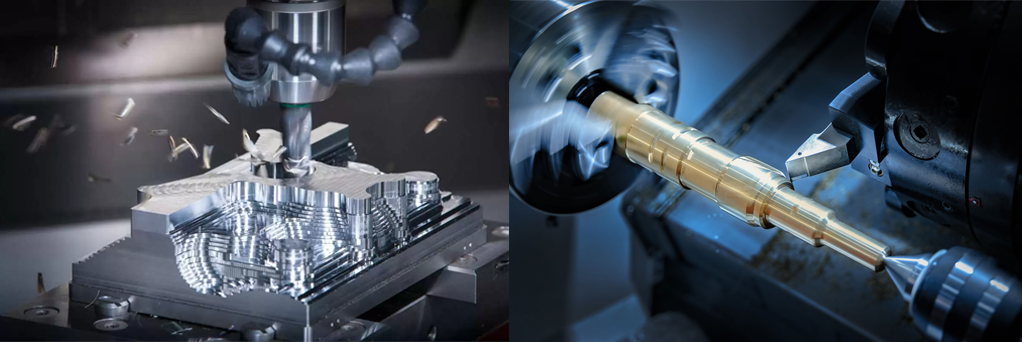
\includegraphics[width=0.6\linewidth]{images/CNCDrehenFraesen.png}
	\caption[CNC-Fräse / CNC-Dreher]{CNC-Fräse / CNC-Dreher}
	\label{fig:CNC Drehen vs Fraesen}
\end{figure}


\subsection{Werkstoffe}
Bei der CNC-Fräsung können die unterschiedlichsten Materialien verwendet werden. Materialien, die eine CNC-Fräse verarbeiten kann, sind zerspanbar  \parencite{PEIZerspannung}. Zu den gängigsten zählen:

\begin{itemize}
	\item Metalle, z. B. Stahl, Aluminium, Titan, Bronze, Messing \parencite{CNCFraesen3}.
	\item Holz
	\item Zerspanbare Kunststoffe, z. B. PEI (\textit{Polyetherimid}), die sich durch ihre mechanische Festigkeit und Steifigkeit auszeichnen \parencite{PEIKunststoffPolyetherimid}.
\end{itemize}

\begin{figure}[H]
	\centering
	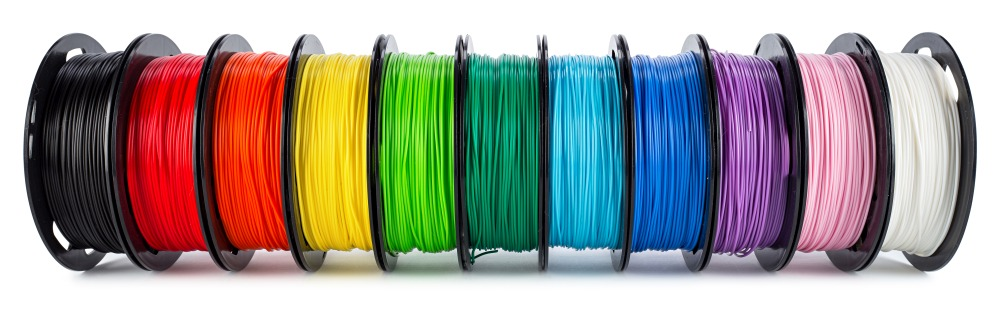
\includegraphics[width=0.5\linewidth]{images/Filamente.jpg}
	\caption[Filamente]{Filamente}
	\label{fig:Kunststoff Filamente}
\end{figure}


\subsection{Fertigungsmöglichkeiten}

\subsubsection{3-Achs-Fräsung}
Hierbei kann sich der Fräser auf drei Achsen bewegen, nämlich auf der X-, Y- und Z-Achse \parencite{Fraesen345Achs}. So kann das Material von allen drei Seiten bearbeitet werden. Es handelt sich um das einfachste Fräsverfahren. Zwar können auch komplexere Objekte erstellt werden, dies erfordert jedoch ein mehrfaches Umspannen des Werkstücks.

\subsubsection{4-Achs-Fräsung}
Zusätzlich zu den bereits bekannten drei Achsen kann nun eine vierte Achse integriert werden, nämlich das Schwenken der Aufspannung des Frästeils \parencite{Fraesen345Achs}. Dadurch kann das Umspannen, das bei der 3-Achs-Fräsung notwendig ist, vermieden werden.

\subsubsection{5-Achs-Fräsung}
Bei der 5-Achs-Fräsung kann nicht nur die Aufspannung des Frästeils zum Schwenken gebracht werden sondern auch der Maschinentisch selbst ist rotierbar. So kann das Werkstück von 5 Seiten in einer Aufspannung bearbeitet werden \parencite{Fraesen345Achs}. Diese Fräsen werden bei der Produktion höchstkomplexer Strukturen eingesetzt.\\

\newpage

\section{3D-Modellierungsprogramme}
Auf dem Markt rund um 3D-Modellierungsprogramme gibt es eine große Auswahl an den verschiedensten Programmen. Vom anfängerfreundlichen Tinkercad, das durch seine einfache Bedienbarkeit und zahlreiche Tutorials überzeugt, bis hin zu einem der führenden CAD-Programme wie Catia  \parencite{3DPrintingSoftware}, das in der Industrie für seine leistungsstarken und umfangreichen Funktionen geschätzt wird. \parencite{CADProgramme} Im Rahmen dieser Diplomarbeit wurden einige der Marktführer recherchiert und miteinander verglichen. \\


\subsection{Vergleich verschiedener Software}

\subsubsection{Autodesk Fusion}
Es eröffnet zahlreiche Anwendungsmöglichkeiten, die von der Prototypenerstellung bis hin zur Entwicklung von Konsumgütern reichen. Dieses Programm bietet umfangreiche Werkzeuge für Design, Engineering und Fertigung.  Fusion 360 wird von vielen internationalen und nationalen Unternehmen verwendet, weil es vielseitig einsetzbar ist und sowohl in kleinen als auch in großen Projekten hervorragende Unterstützung bietet. \parencite{AutodeskFusion}. Dank seiner cloudbasierten Plattform ermöglicht Fusion 360 eine nahtlose Zusammenarbeit und den einfachen Austausch von Projektdaten, was es zu einer bevorzugten Wahl in der modernen Produktentwicklung macht. \\

\textbf{Vorteile}
\begin{itemize}
	\item Genutzt von vielen namhaften Unternehmen wie zb. Yamaha oder Panasonic
	\item Große Community
	\item Kostenlose Version für Schulen \parencite{AutodeskFusionReviews}
\end{itemize} 

\textbf{Nachteile}
\begin{itemize}
	\item Cloud Based; Kann zu Problemen führen, wenn offline genutzt 
	\item Benötigt eine schnelle Internetverbindung
	\item Hoher Anspruch an die Hardware des Computers \parencite{AutodeskFusionReviews}
\end{itemize}

\begin{figure}[H]
	\centering
	
\includegraphics[width=0.3\linewidth]{images/Fusion360.png}
	\caption[Fusion360]{Fusion360}
	\label{fig:Autodesk Fusion}
\end{figure}



\subsubsection{Blender} 
Blender bietet vielseitige Anwendungsmöglichkeiten, von Modellierung und Animation bis hin zur Spieleentwicklung und visuellen Effekten. Dieses Open-Source-Programm bietet umfassende Werkzeuge für Modellierung, Simulation, Rendering, Compositing und Motion Tracking. Zudem wird Blender von vielen internationalen und nationalen Unternehmen sowie privaten Kunden bzw. Kundinnen verwendet, weil es viele Einsatzmöglichkeiten bietet und gratis zugänglich ist \parencite{Blender}. Dank seiner aktiven Community und regelmäßigen Updates bleibt Blender immer auf dem neuesten Stand der Technik. \\


\textbf{Vorteile}
\begin{itemize}
	\item Gratis 
	\item Open Source Software
	\item Funktioniert auf allen gängigen Betriebssystemen
	\item Regelmäßige Updates
	\item große Community \parencite{BlenderProsUndCons}
\end{itemize}

\begin{figure}[H]
	\centering
	
\includegraphics[width=0.3\linewidth]{images/Logo_Blender.png}
	\caption[Blender Logo]{Blender Logo}
	\label{fig:Blender}
\end{figure}


\textbf{Nachteile}
\begin{itemize}
	\item Kein Industriestandard - wird nicht von großen Unternehmen genutzt
	\item Nicht die benutzerfreundlichste Oberfläche \parencite{BlenderProsUndCons}
\end{itemize}



\subsubsection{FreeCAD}
FreeCAD hat vielseitige Anwendungsmöglichkeiten, von der Modellierung bis hin zur Erstellung technischer Zeichnungen und Simulationen. Diese Open-Source-Software bietet umfassende Werkzeuge für Ingenieure, Architekten, Produktdesigner und Privatkunden \parencite{FreeCAD}. Zudem wird FreeCAD von vielen Unternehmen sowie unabhängigen Entwicklern und Entwicklerinnen genutzt. Durch seine modulare Architektur und der aktiven Community wird FreeCAD kontinuierlich weiterentwickelt und verbessert.   \parencite{FreeCAD2}. \\


\textbf{Vorteile}
\begin{itemize}
	\item Open Source Software
	\item Gratis
	\item Funktionsfähig für alle gängigen Betriebssysteme
	\item Aktive Community \parencite{FreeCADReviews}
\end{itemize}

\textbf{Nachteile}
\begin{itemize}
	\item weniger Nutzer und Nutzerinnen als die bereits genannten Programme
	\item kein Industriestandard
	\item limitierte Funktionalitäten im Vergleich zu Bezahlsoftware \parencite{FreeCADReviews}
\end{itemize}

\subsubsection{Autodesk Tinkercad}
Autodesk Tinkercad ist ein für Anfänger und Anfängerinnen und Schüler und Schülerinnen entwickeltes Online-Tool. Wie der Name es schon verrät, ist es ein Produkt von Autodesk, wie das vorher genannte Autodesk Fusion 360. Dieses webbasierte Programm erfüllt alle grundlegenden Anforderungen und bietet intuitive Werkzeuge für Schüler und Schülerinnen, Lehrer und Lehrerinnen und Privatpersonen. Zudem wird Tinkercad von vielen Bildungseinrichtungen verwendet, weil es leicht zugänglich und einfach zu erlernen ist \parencite{Tinkercad}. Dank seiner klaren Benutzeroberfläche und umfangreichen Tutorials ermöglicht Tinkercad einen schnellen Einstieg in die Welt des 3D-Designs und der Elektronik. \\


\textbf{Vorteile}
\begin{itemize}
	\item Gratis
	\item Benutzerfreundliches UserInterface
	\item intuitives Design
	\item Online Tool - kein Download 	
	\item viele einsteigerfreundliche Tutorials \parencite{TinkercadReviews}
\end{itemize}

\textbf{Nachteile}
\begin{itemize}
	\item Weniger professionell
	\item kein Industriestandard \parencite{TinkercadReviews}
\end{itemize}

\section{Mischpult}
Für StageControl benötigen wir zur Ansteuerung einer Tonanlage ein Mischpult, um den von uns gewünschten Stereoeffekt zu erzeugen. Mischpulte, auch Mixer genannt, gibt es in ganz unterschiedlichen Größen. Das Ausmaß hängt meist von der Anzahl der Kanäle ab, die das Mischpult bietet. Diese technologie wird immer dann verwendet, wenn mehrere Audiosignale verarbeitet werden müssen, wie auf Bühnen. \parencite{MischpultInformation} Bei allen Mischpulten gibt es eine sogenannte Leserichtung, die den Aufbau des Mischpults beschreibt. Von links nach rechts findet man die einzelnen Kanäle, und von oben nach unten die Bearbeitungsmöglichkeiten des Tons. Dazu kommt noch der sogannte Masterbereich. Hier wird alles gesteuert, was zentral gereglt werden muss. Diese Einstellungen gelten dann für alle Kanäle.  \parencite{MischpultMaster} \\


\begin{figure}[H]
	\centering
	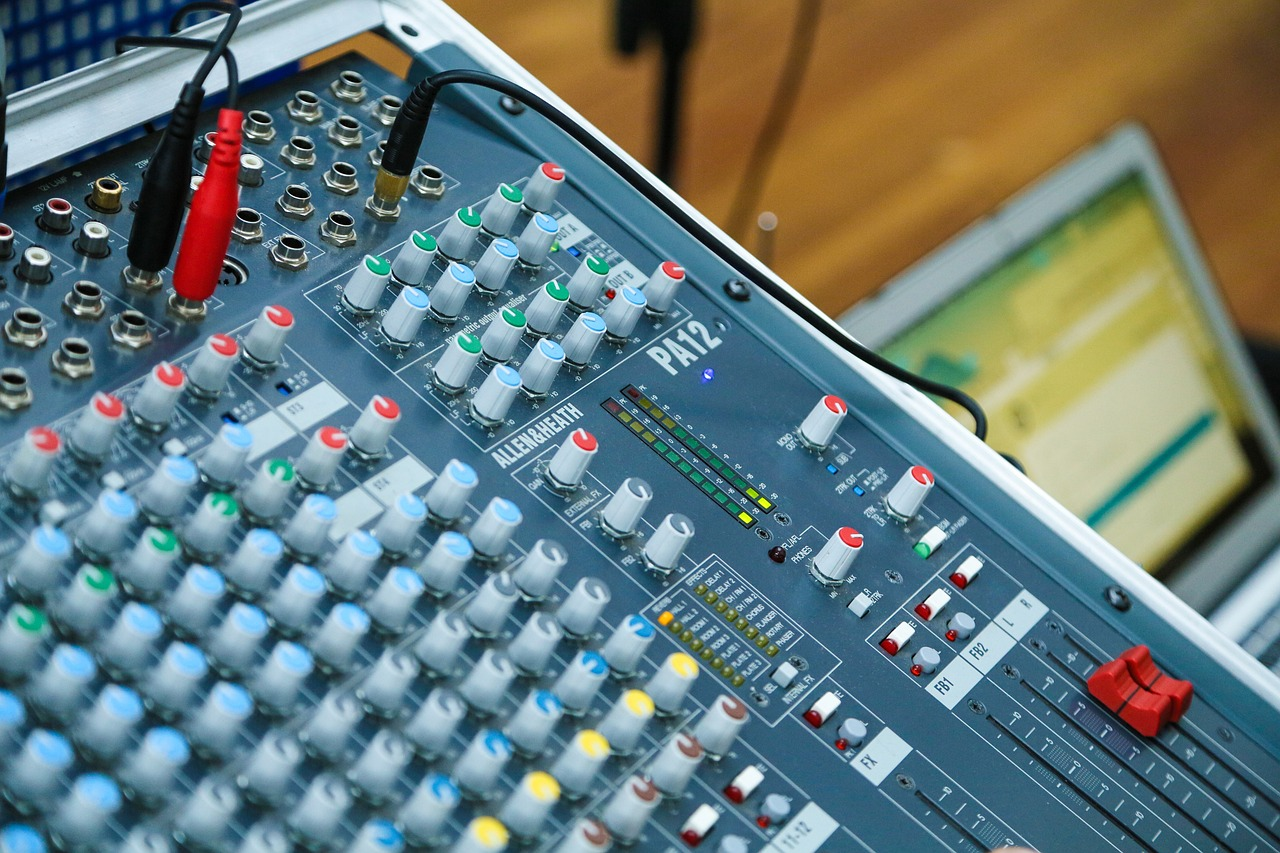
\includegraphics[width=0.6\linewidth]{images/mischpult.jpg}
	\caption[Mischpult]{Mischpult}
	\label{fig:Mischpult}
\end{figure}

\subsection{Funktionsweise eines Mischpults}
Im Grunde summiert ein Mischpult alle Tonquellen zu einen einzigen Signal. So kann dann dieses Signal über die Tonanlage ausgegeben werden \parencite{MischpultErklaerung}. Bei Mischpulten gibt es eine Vielzahl von Knöpfen und Reglern für jeden Kanal, diese sind wie schon erwähnt zur Bearbeitung des Tones da, im Rahmen dieser Diplomarbeit wird auf dies nicht genauer eingegangen. \\


\subsection{Einsatzmöglichkeiten}
Mischpulte finden eine Vielzahl von Anwendungsmöglichkeiten, wie z.B. auf Bühnen oder in Proberäumen. Mischpulte übernehmen eine Bandbreite von Aufgaben \parencite{MischpultVerwendungszweck}. Die folgenden gehören zu den Wichtigsten:
\begin{itemize}
	\item Signalverstärkung
	\item Bearbeitung von Signalen
	\item Signale zum Aufnahmesystem schicken
\end{itemize}


\subsection{Unterschied Digital/Analog}
\subsubsection{Digital}
Unter einem digitalen Mischpult versteht man ein Mischpult, das analoge Signale in digitale Signale umwandelt und diese Signale mittels Software bearbeitet. Um ein digitales Signal wieder über eine Tonanlage auszugeben, muss es erneut in ein analoges Signal umgewandelt werden. Dies führt wiederum zu Latenzzeiten bei der Signalausgabe.
\subsubsection{Analog}
Im Gegensatz dazu steht das analoge Mischpult. Es wandelt die Signale nicht in digitale um, sondern behält deren ursprüngliche analoge Form bei und bearbeitet sie ohne Software weiter \parencite{MischpultAnalogDigital}. Ohne diese Umwandlung gibt es nahezu keine Latenzzeit bei der Ausgabe der Signale. \\


\begin{figure}[H]
	\centering
	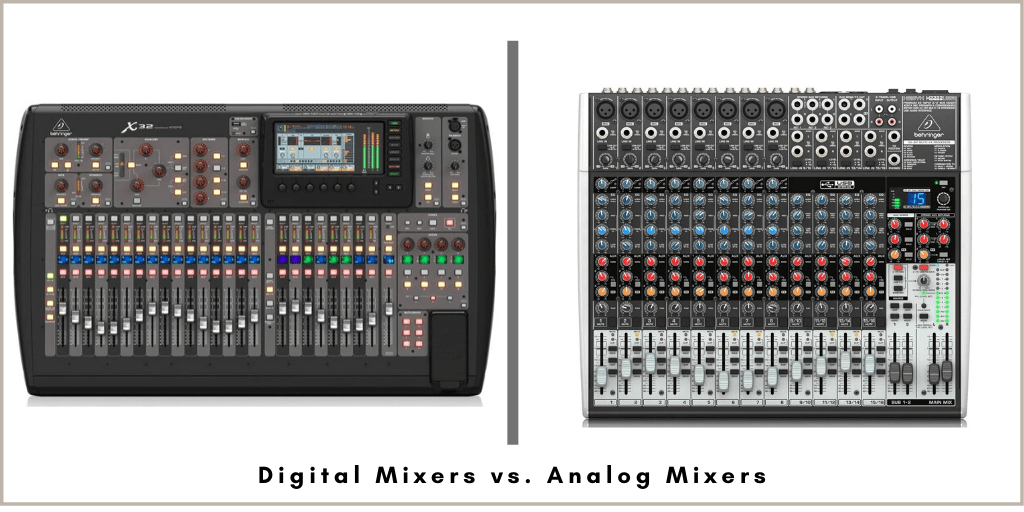
\includegraphics[width=0.8\linewidth]{images/DigitalMixerAnalogMixer.png}
	\caption[Digitales vs Analoges Mischpult]{Digitales vs Analoges Mischpult}
	\label{fig:Digitales vs. Analoges Mischpult}
\end{figure}


\subsection{Anforderungen für StageControl}
Für StageControl ist es besonders wichtig, dass das verwendete Mischpult entweder jeden Kanal einzeln panen (\textit{Regler zu Ausrichtung des Tons (links/Rechts)}) kann oder das der Master mindestens zwei Lautsprecher einer Tonanlage einzeln ansteuern kann. Somit kann der von uns gewünschte Stereoeffekt erzeugt werden. \\
Für StageControl wird ein Mischpult mit Drehreglern verwendet, da diese häufig in kostengünstigeren Mischpulten zu finden sind und für die Anforderungen dieser Arbeit vollkommen ausreichen. 



\subsection{Vergleich zweier Modelle}
Wie am Anfang des Kapitels \textit{Mischpult} beschrieben benötigt StageControl ein Mischpult, um den von uns gewünschten Stereoeffekt zu erzeugen. Hierzu werden zwei Mischpulte herangezogen \parencite{MischpultKriterien1204}, die unseren Kriterien entsprechen und  verglichen  \parencite{MischpultKriterien1402}.

\begin{table} [H]
	\begin{tabular}{ |p{3.1cm} |p{4.8cm}|p{4.8cm}| }
		\hline
		\textbf{Kriterien} & \textbf{Behringer Xenyx 1204USB}& \textbf{the t.mix xmix 1402 USB}\\
		\hline
		\textbf{Kosten} & 169€ & 168€  \\ 
		\hline
		\textbf{Digital/Analog} & Analog & Analog   \\  
		\hline
		\textbf{Master kann zwei Lautsprecher seperat ansprechen} & Ja & Ja \\
		\hline
		\textbf{PC-Schnittstelle} & USB-B & USB-B  \\
		\hline
		\textbf{Gewicht}& 2.8 kg & 4.8 kg \\
		\hline	
	\end{tabular}
	\caption{Vergleich Behringer Xenyx 1204USB und the t.mix xmix 1402 USB} 
\end{table} 

\begin{figure}[H]
	\centering
	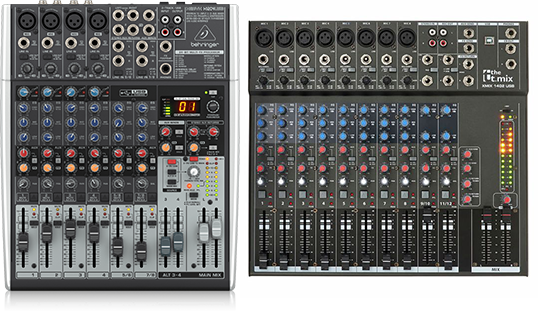
\includegraphics[width=0.8\linewidth]{images/the.t.mix.xmix1402-Behringer1204USB.png}
	\caption[Vergleich Behringer Xenyx 1204USB und the t.mix xmix 1402 USB]{Vergleich Behringer Xenyx 1204USB und the t.mix xmix 1402 USB}
	\label{fig:Behringer Xenyx 1204USB-the t.mix xmix 1402 USB}
\end{figure}

\section{Lichtsteuerung}
Ein weiterer Aspekt dieser Diplomarbeit ist die gleichzeitige Ansteuerung von Ton- und Lichtanlagen, wie z.B. einem Spotlight (\textit{deutsch Verfolgungsscheinwerfer}), das den Künstler bzw. die Künstlerin auf der Bühne verfolgt. Auf Bühnen wird nicht nur ein Spotlight eingesetzt, sondern ganze Anlagen von Lichtern. 

\begin{figure}[H]
	\centering
	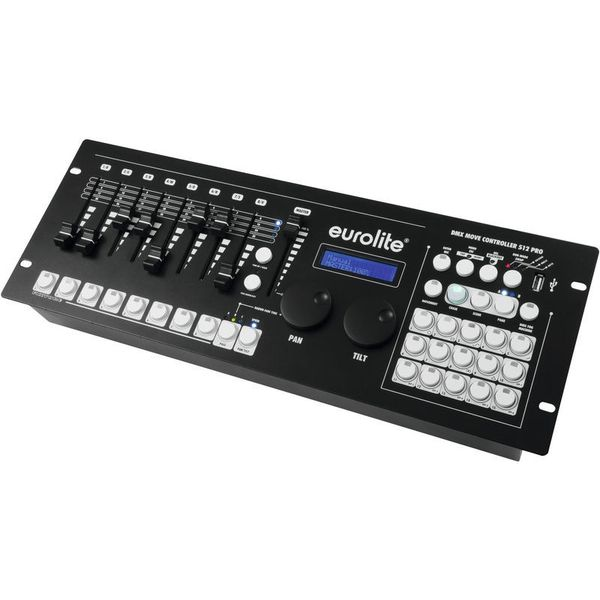
\includegraphics[width=0.7\linewidth]{images/DMXController.jpg}
	\caption[DMX Controller]{DMX Controller}
	\label{fig:DMXController}
\end{figure}

\subsection{Lichtanlagen bei StageControl}
Im Fall von StageControl wird keine vollständige Lichtanlage verwendet; es kommt lediglich ein Scheinwerfer zum Einsatz, um die Beleuchtung der Künstler bzw. der Künstlerinnen via Positionsverfolgung zu ermöglichen. So erhalten wir die genaue Abstimmung von Ton und Licht auf die Person.

\subsection{Ansteuerung von Lichtanlagen}

Die gängigsten Arten der Ansteuerung von Lichtanlagen sind das DMX-Protokoll (\textit{Digital Multiplex}) oder das RDM-Protokoll (\textit{Remote Device Management}). Zur Ansteuerung der Lichtanlagen selbst wird ein DMX-Controller benötigt, der die Scheinwerfer steuert. Es wird ein DMX-Controller mit einem DMX-Ausgang und ein Scheinwerfer mit einem DMX-Eingang gebraucht.
\textbf{DMX} ist das am häufigsten verwendete Protokoll zur Lichtansteuerung in der Bühnentechnik. Moving-Heads, Lichteffekte und viele mehr werden in der Regel mithilfe von Lichtsteuerpulten über das DMX-Protokoll angesteuert und/oder programmiert \parencite{LichtanlageRDMDMX}.
\textbf{RDM} basiert auf dem DMX-Protokoll, erlaubt aber im Halbduplexbetrieb Rückmeldungen, was das Einrichten deutlich erleichtern kann.\\


\subsection{Hartes bzw. weiches Licht}
Es gibt zwei Lichtarten, die man in der Lichttechnik unterscheiden kann, nämlich hartes und weiches Licht. Beide Arten bieten sich für unterschiedliche Einsatzmöglichkeiten an. Weiches Licht wird meist eingesetzt, um größere Bereiche auszuleuchten. Im Gegensatz zu weichem Licht gibt es hartes Licht, das sehr präzise eingesetzt werden kann, wie im Fall von StageControl bei der Verfolgung des Künstlers oder der Künstlerin auf einer Bühne. Bei Scheinwerfern, die hartes Licht ausstrahlen, strahlt das Licht von einem Punkt aus \parencite{HartesWeichesLicht}. Hingegen wird weiches Licht von einer Fläche aus abgestrahlt.\\


\subsection{Arten von Scheinwerfern}
In der Lichttechnik gibt es verschiedenste Scheinwerfertypen, die unterschiedliche Aufgaben besonders gut erfüllen. Zwei Scheinwerfertypen, die im Rahmen dieser Diplomarbeit zum Einsatz kommen, werden genauer erklärt.

\subsubsection{Verfolgerscheinwerfer}
Der Verfolgerscheinwerfer wird verwendet, um Personen auf Bühnen zu verfolgen. Diese Scheinwerfer werden nicht wie andere Scheinwerfer fix montiert, sondern lassen sich bewegen, um den gewünschten Verfolgungseffekt zu bieten. Dies geschieht nicht automatisch, sondern wird manuell von einem Beleuchter während der Show durchgeführt \parencite{Verfolgerscheinwerfer}. Es gibt verschiedene Lösungsansätze zur Bewegung von Movinglights (\textit{deutsch „Bewegbare Lichter“}).  Bei Konzerten wird ein Verfolgerscheinwerfer oberhalb der Bühne gemeinsam mit dem Beleuchter platziert. Dieser steuert dann das Licht über ein Bedienfeld während der Performance.\\


\begin{figure}[H]
	\centering
	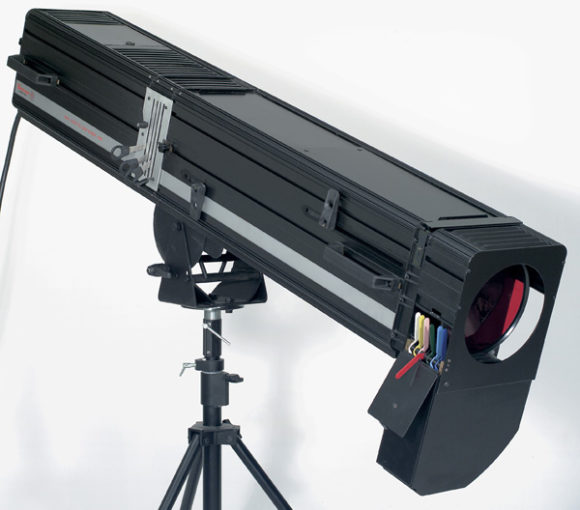
\includegraphics[width=0.4\linewidth]{images/Verfolgerscheinwerfer.jpg}
	\caption[Verfolgerscheinwerfer]{Verfolgerscheinwerfer}
	\label{fig:Verfolgerscheinwerfer}
\end{figure}

\subsubsection{Profilscheinwerfer}
Dieser Scheinwerfertyp wird vor allem im Theaterbereich eingesetzt. Ein enormer Vorteil des Profilscheinwerfers ist, dass er ein hartes und exaktes Licht ausstrahlt. Außerdem ist das Streulichtaufkommen deutlich geringer als bei anderen Scheinwerfern. Streulicht ist das Licht, das außerhalb des eigenlichen Lichtkegels auftritt. Zudem verfügen Profilscheinwerfer über einen Zoom, der manuell oder automatisch erfolgen kann \parencite{Profilscheinwerfer}. Dieser Scheinwerfertyp bietet zusätlich eine Scharfstellfunktion/Fokus mittels Linsenverschiebung an, diese wird durch den Linsentubus ermöglicht.\\


\begin{figure}[H]
	\centering
	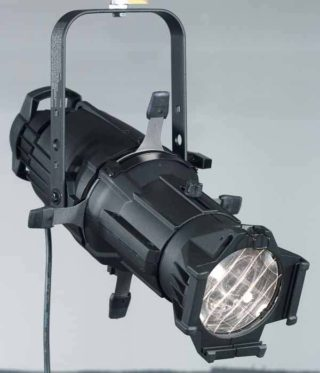
\includegraphics[width=0.4\linewidth]{images/Profilscheinwerfer.jpg}
	\caption[Profilscheinwerfer]{Profilscheinwerfer}
	\label{fig:Profilscheinwerfer}
\end{figure}

\section{Servomotoren}
\subsection{Einsatz von Servos bei StageCotrol}
Servomotoren werden für die Umwandlung der physischen Bewegung des Künstlers, in mechanische Bewegung des Servomotors benötigt, um so die Regler des Mischpults in Abstimmung und Ausrichtung des Künstlers mit dem Ton zu automatisieren. Diese Servomotoren werden oberhalb des Mischpult mithilfe des Gerüsts plaziert, wie in Kapitel 2.2.1 beschrieben.

\subsection{Was ist ein Servomotor}
Unter einem Servomotor wird keine Bauart eines Motors verstanden, sondern vielmehr spezielle Eigenschaften. Diese Eigenschaften sind: Strom-, Drehzahl- und/oder Positionsgeregelt. Ein Servomotor ist immer elektrisch betrieben. Diese Motoren geben Rückmeldungen an die Regelelektronik. Diese Rückmeldungen enthalten Informationen über Winkelposition der Motorwelle, der Drehgeschwindigkeit und der Beschleunigung \parencite{ServomotorInfo}. Die Regelelektronik kann anhand dieser zurückgemeldeten Daten wieder die Daten der Sollparameter an den Motor schicken, die zuvor eingegeben wurden. \\


\subsection{Anforderungen für StageControl}
Für den Einsatz bei StageControl gibt es Vorraussetzungen, die die Servomotoren erfüllen müssen, ehe sie in Erwägung gezogen werden. Diese Kriterien sind: Drehung des Motors im und gegen den Uhrzeigersinn, Kompaktheit, passenende Schnittstelle (Bus/Analog/Digital) für die Eingabe der Sollzustände und die Rückmeldung der Aktuellen Position.

\begin{figure}[H]
	\centering
	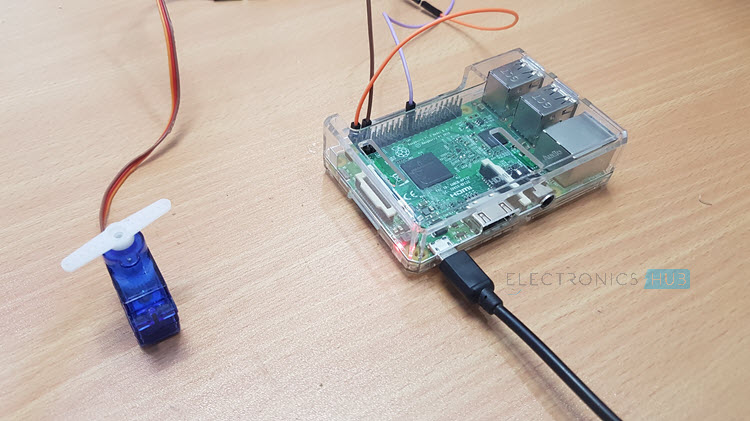
\includegraphics[width=0.7\linewidth]{images/servo.jpg}
	\caption[Servomotor]{Servomotor}
	\label{fig:Servo}
\end{figure}

\subsection{Arten von Servomotoren}
Es gibt einige unterschiedliche Arten von Servos, die wichtigsten drei sind: Gleichstrom, kernlose und bürstenlose Motoren. \\
Bei Gleichstromservos handelt sich um die billigste und gängiste Art der Motoren. Dieser Servotyp besteht aus Eisenkernen um die Kupferdraht gewickelt ist, sowie einem Kommutator Ring und Bürsten. Diese Bürsten werden zur Umschaltung der Felder benötigt und einem Gehäuse. \\
Kernlose Motoren sind erheblich teuerer in der Produktion als Gleichstrommotoren, da diese aus teurern Materialien bestehen. Ihr großer Vorteil gegenüber herkörmlicher Gleichstrommotoren ist, das diese deutlich schneller beschleunigen und abbremsen können \parencite{ServomotorArten}. \\
Anstelle der Bürsten und dem Metallring bei Bürstenservos, wird bei den Bürstenlosen Servos Elektronik, die den Motor steuert, eingebaut um die selbe Zuverlässigkeit zu gewährleisten. Der Einbau von Elektronik zeichnet sich durch die längere Lebensdauer des Servos aus. Durch die Elektronik fallen diese Motoren deutlich teurer aus als Gleichstrommotoren. \\

\begin{figure}[H]
	\centering
	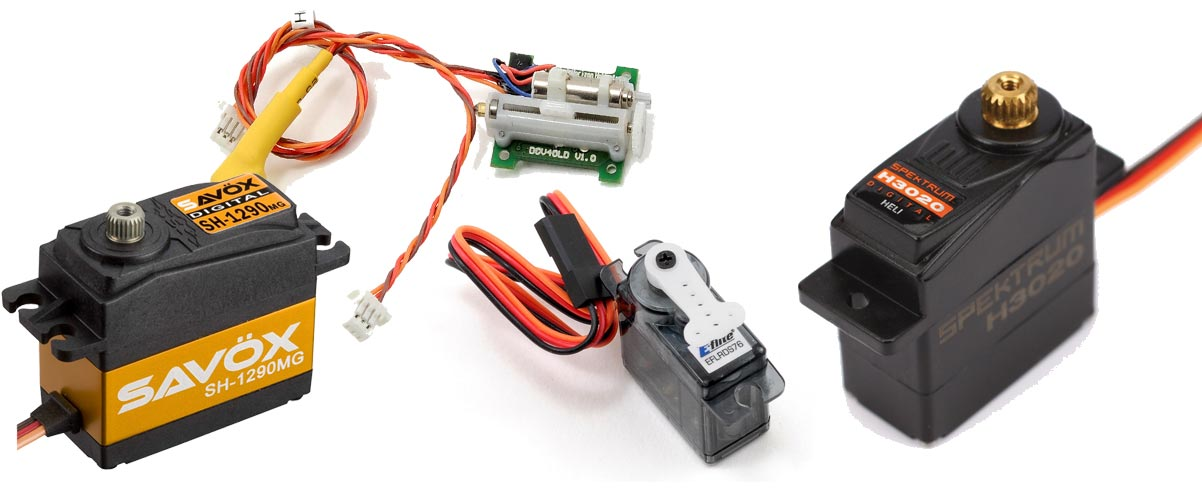
\includegraphics[width=0.5\linewidth]{images/ServoArten.jpg}
	\caption[Servo Arten]{Servo Arten}
	\label{fig:Servo Arten}
\end{figure}



\subsection{Ansteuerung von Servos}
Servomotoren werden über ein sogenanntes PWM-Signal (\textit{Pulsweitenmodulations-Signal}) gesteuert. Dies bedeutet, dass der Servomotor über elektrische Pulse angesteuert wird und so die Befehle erhält, auf welche Postion er fahren muss. Diese Motoren werden üblicherweise über drei Kabeln mit dem Steuerunggerät verbunden. Das erste Kabel ist das Massekabel, es ist für die Rückleitung der Pulse verantwortlich. Nummer zwei ist das Versorgungsspannungskabel, das den Servomotor mit der nötigen elektrischen Spannung versorgt. \parencite{ServomotorAnsteuerung}. Das dritte Kabel ist das Signalleitungskabel, dieses  leitet die Pulse an den Servo weiter, so wird dem Servo die anzufahrende Position mitgeteilt.\\


\begin{figure}[H]
	\centering
	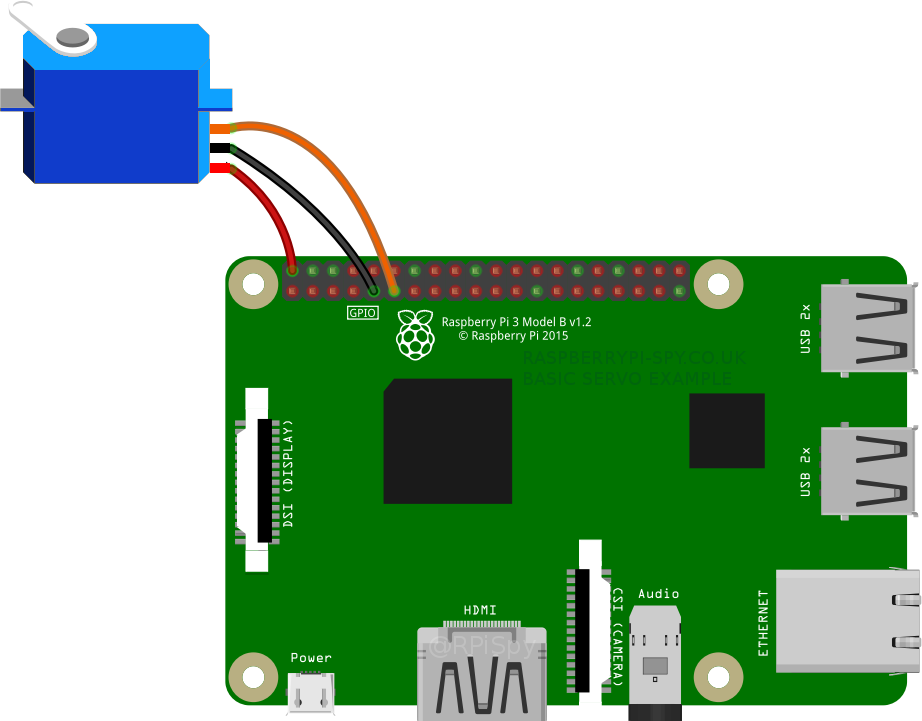
\includegraphics[width=0.7\linewidth]{images/Pin_Belegung.png}
	\caption[Pin-Belegung Servo]{Pin-Belegung Servo}
	\label{fig:PIN_Belegung}
\end{figure}

\section{Navigation}

Um die Licht- und Audioanlagentechnik richtig zu koordinieren benötigt man eine Art von Navigation. Da es sich meist um Bühnen im Innenbereich handelt, kann man keine übliche Technologie verwenden.


\subsection{GPS}
GPS (\textit{=engl. Global Positioning System}) ist ein globale Navigationssystem, das die Bestimmung von Standort, Geschwindigkeit und Zeit ermöglicht und synchronisiert. Es wird für heutzutage fast überall verwendet im Auto, Smartphone oder Uhr und hilft dabei von A nach B zu gelangen. \parencite{GPS} Da zu aktuellem Zeitpunkt eine Standortermittlung indoor über GPS zu ungenau ist (um den Faktor 100 mehr gedämpft) können wir GPS nicht verwenden. \textcite{Indoor}

\textbf{Funktionsweise Global Navigation Satellite System}

Das Global Navigation Satellite System \textit{(=GNSS)} verwendet eine Technik namens Trilateration, diese benötigt zur Berechnung von Standort Geschwindigkeit und Höhe, Signale von Satelliten, um Positionen anzugeben. 

Die erwähnten Satelliten, umkreisen die Erde und senden Singale, die von den jeweiligen GPS-Geräten auf der Erdoberfläche ausgewertet werden. Das Gerät muss das Signal von mindestens vier Satelliten lesen können, um die Position korrekt zu berechnen. \parencite{GPS} 

Durch die Positionsermittlung können folgende andere Informationen berechnet werden:

\begin{itemize}
	\item Geschwindigkeit
	\item Peilung
	\item Track
	\item Reisedistanz
	\item Distanz zum Ziel
	\item Zeiten von Sonnenauf- und untergang
\end{itemize}

\textbf{Fehlerquellen für die Genauigkeit der GPS-Signale}

Es gibt einige relevante Fehlerquellen für GPS-Signale, darunter fallen \parencite{GPSFehlerquellen}:
\begin{itemize}
	\item Position der Satelliten
	\item Signaleffekt der Umgebung
\end{itemize}


\textbf{Position der Satelliten}

Um ein Objekt zu positionieren sind mindestens drei Satelliten notwendig und ein weiterer, um etwaige Fehler zu beseitigen. Grundsätzlich gilt: Je mehr Satelliten, desto besser die GPS-Genauigkeit. Außerdem sollte das Signal von gleichmäßig verteilten Satelliten kommen, dann ist die GPS-Genauigkeit höher. Für die Berechnung dieser Genauigkeit gibt es den Dilution of Precision (= DOP) Wert.  Je kleiner dieser Wert, desto genauer ist das GPS-Signal.
\begin{figure}[H]
	\centering
	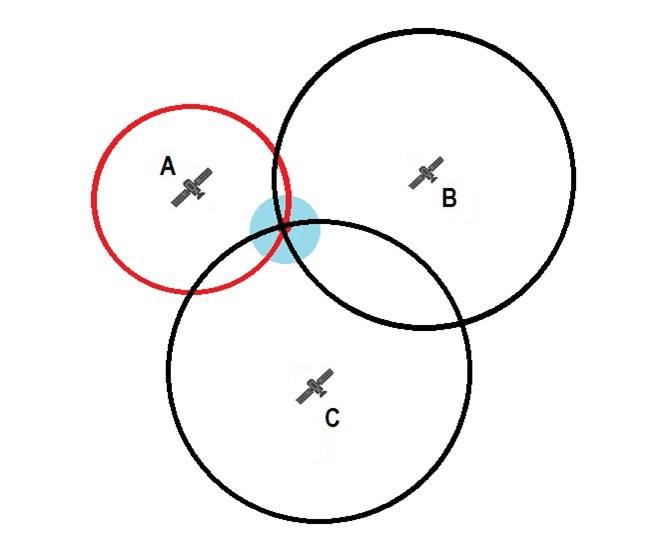
\includegraphics[width=0.7\linewidth]{images/Satellitenposition.jpg}
	\caption[Satellitenpositionierung]{Satellitenpositionierung}
	\label{fig:Satellitenposition}
\end{figure}

\textbf{Signaleffekt der Umgebung}


Bis die Signale von Satelliten schlussendlich beim GPS-Empfänger ankommen legen sie eine lange Strecke zurück. Die Ausbreitungsumgebung beeinflusst nicht nur die Signalstärke, sondern auch die Genauigkeit.

Um aktuell eine GPS-Genauigkeit von 5-10 Metern zu gewährleisten, muss das Signal von möglichst vielen Satelliten gleichzeitig empfangen werden. Je mehr Satelliten desto genauer ist die Ortung möglich. In Gebäuden, wo kein GPS-Signal empfangbar ist, kann man nicht mit einer genauen Standortbestimmung rechnen. \parencite{GPSGenauigkeit}

\begin{figure}[H]
	\centering
	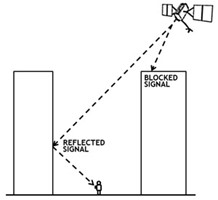
\includegraphics[width=0.7\linewidth]{images/Satelliteneinfluss.jpg}
	\caption[Satelliteneinfluss]{Satelliteneinfluss}
	\label{fig:Satelliteneinfluss}
\end{figure}

\subsection{ESP32}

ESP32 ist eine Reihe von Chip-Mikrocontrollern, die von dem Unternehmen Espressif entwickelt wurden und mit Hilfe von Arduino bzw. der Programmiersprache C kommunizieren. Der ESP32 \textcite{ESP32} zeichnen sich mit folgenden Dingen aus:

\begin{itemize}
	\item niedrige Anschaffungskosten
	\item geringer Stromverbrauch
	\item Wi-Fi
	\item Bluetooth
\end{itemize}


\begin{figure}[H]
	\centering
	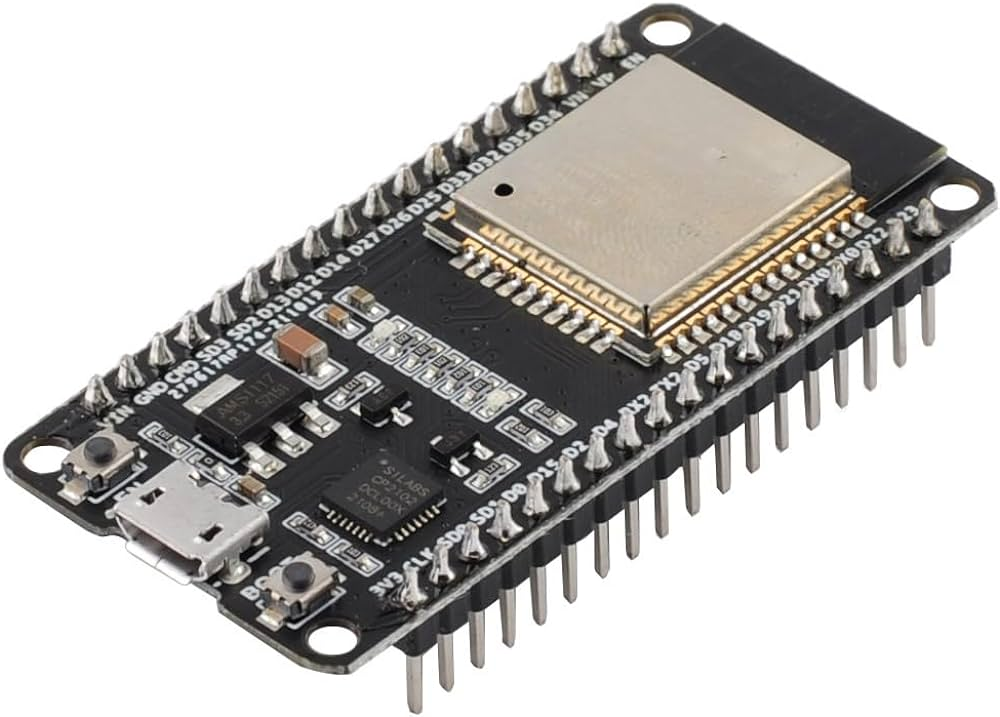
\includegraphics[width=0.7\linewidth]{images/ESP32.jpg}
	\caption[ESP32]{ESP32}
	\label{fig:ESP32}
\end{figure}

\textbf{Anschaffungskosten \& Stromverbrauch}

Der Mikrocontroller ist bereits ab einem Preis von 6\$ erhältlich. Außerdem verbraucht dieser im Vergleich zu anderen Mikrocontrollern sehr wenig Strom und unterstützt Energiesparmodule, wie Tiefschlaf.

\textbf{Funktionen}

Der Mikrocontroller bietet nicht nur Wi-Fi (\textit{=Wireless Local Area Network}), sondern auch Bluetooth. Mit der Wireless Local Area Network Funktion kann man einfach und drahtlos eine Verbindung zu einem Netzwerk herstellen und somit eine Kommunikation von vielen Geräten möglich machen. Außerdem verfügt der Mikrocontroller über Bluetooth-Classic.

\subsection{ESP32-Spezifikationen}

\begin{itemize}
	\item Bluetooth Classic und Bluetooth Low Energy
	\item Tensilica Xtensa Dual-Core 32-Bit LX6 Mikroprozessor, 160 oder 240 MHz
	\item ROM:  448 KB
	\item SRAM:  520 KB 
\end{itemize}

\subsection{MPU-6050}

Für weitere Funktionen benötigt man z.B. die Erweiterungsplatine MPU-6050, diese bringt einen Beschleunigungssensor und ein Gyroskop mit. Diese Platine beläuft sich auf einen Preis von ca. \$3.

\begin{figure}[H]
	\centering
	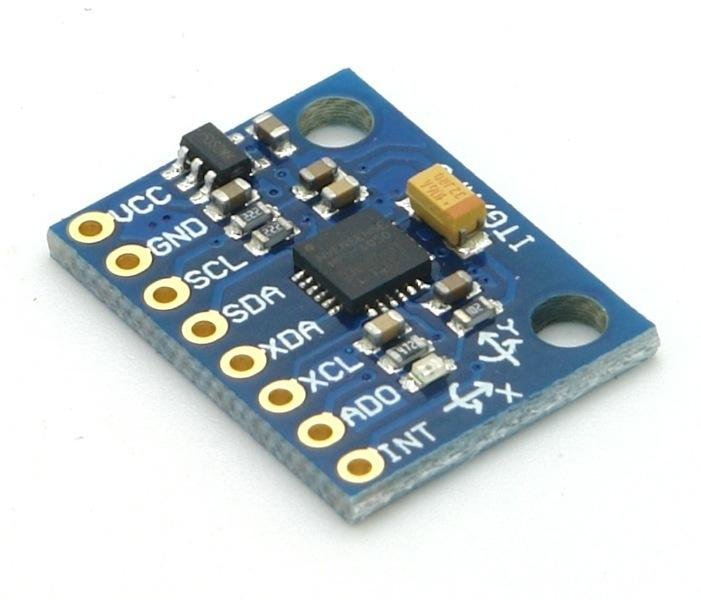
\includegraphics[width=0.7\linewidth]{images/MPU6050.jpg}
	\caption[MPU6050]{MPU-6050}
	\label{fig:MPU6050}
\end{figure}


\textbf{Gyroskop}

Ein Gyroskop ist wie ein Kreisel aufgebaut und hat somit die selbe Wirkung und wird deshalb auch Kreiselinstrument genannt. Man nutzt die Wirkung, um die Lage eines Objektes zu bestimmen. Im Falle von einem MPU-6050 wird ein Sensor namens Micro-Electric-Mechanical Systems (\textit{kurz MEMS}) verwendet. 


\begin{figure}[H]
	\centering
	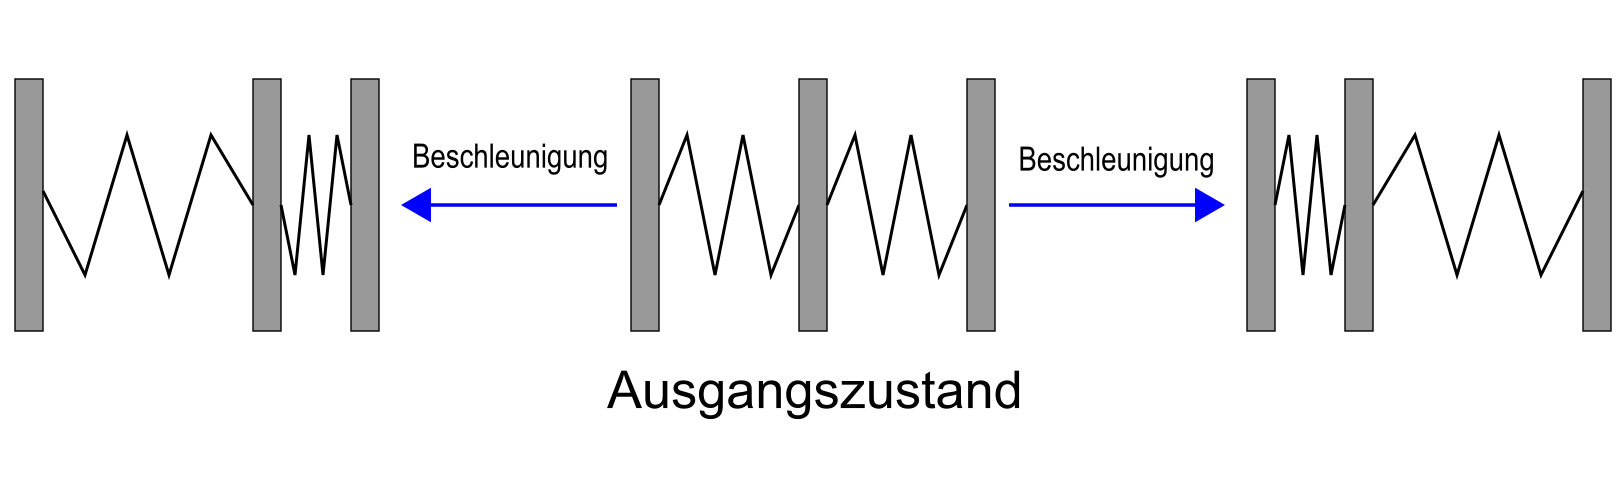
\includegraphics[width=0.7\linewidth]{images/Beschleunigungssensor.png}
	\caption[Beschleunigungssensor]{Beschleunigungssensor}
	\label{fig:Beschleunigungssensor}
\end{figure}

\textbf{Beschleunigungssensor}

Ein Beschleunigungssensor funktioniert nach dem selben Prinzip, wie ein Gyroskop. Der einzige Unterschied ist, dass der Sensor die Beschleunigung in Richtung der x-, y- und z-Achse deklariert. Ein Gyroskop bezieht sich lediglich auf die Bewegung, um die Achsen, also befindet es sich in Ruhestellung und liefert den Wert Null für alle drei Dimensionen (x,y,z). \textcite{MPU6050} Die Module haben die Achsen aufgedruckt.

\begin{figure}[H]
	\centering
	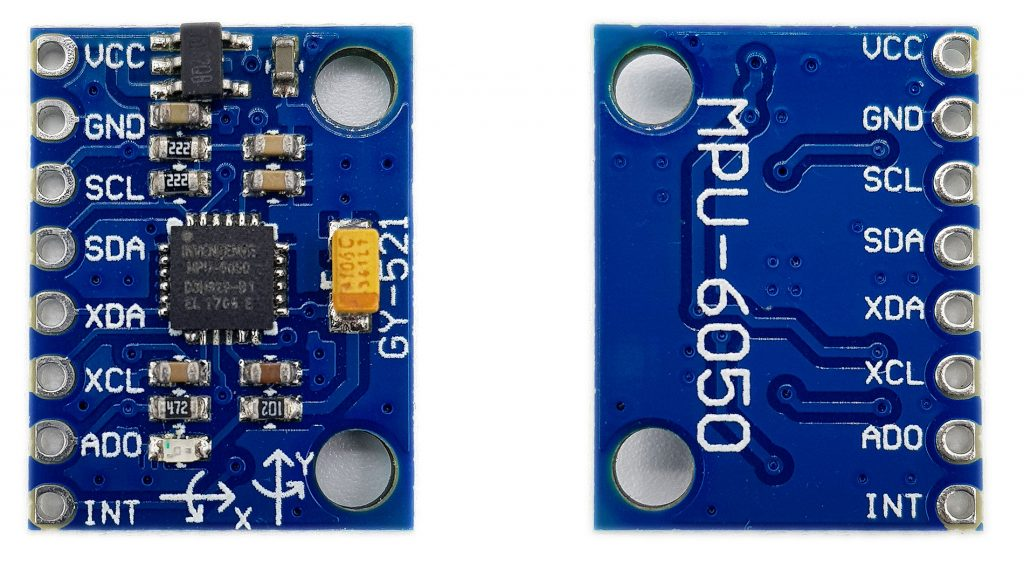
\includegraphics[width=0.7\linewidth]{images/Modul.jpg}
	\caption[Modul]{Modul}
	\label{fig:Modul}
\end{figure}

\subsection{Trägheitsnavigation}

Die Trägheitsnavigation nutzt die physikalische Eigenschaften der Trägheit, um fortlaufende Berechnung der Position, Orientierung und Geschwindigkeit eines Objekts zu ermöglichen. \parencite{Traegheitsnavigation} Es ist immer nur die Anfangsposition bekannt, anhand dieser wird die spätere Position eines Objektes errechnet. Auch in GPS-gestörten Umgebungen z.B. Gebäuden, funktioniert die Trägheitsnavigation. 


\section{Software}


\subsection{Mobil Apps Grundlagen}

\textbf{Native Apps}

Native Apps (\textit{=deu.: angepasste Anwendung}) sind Anwendungen, die speziell für ein Betriebssystem (Android, iOS) entwickelt wurden.

\textbf{Android}

Android ist einer der weltweit bekanntesten Betriebssysteme. Das Betriebssystem fasst einen weltweiten Marktanteil von 71.31\% im April 2024. \parencite{AndroidVsiOS} Weiters ist Android ein Open-Source Betriebssystem, es ist offen für Entwickler.  

\textbf{iOS}

Das Betriebssystem iOS wurde von Apple im Jahre 2007 veröffentlicht und hat im April 2024 einen weiltweiten Marktanteil von 27.95\%. \parencite{AndroidVsiOS} Die Software wird auf den entwickelten Geräten von Apple verwendet. Anders wie bei Android ist iOS nicht quelloffen, außerdem werden keine Betriebssystem-Lizenzen vergeben. Man benötigt eine gültige Apple-ID, um das Gerät zu verwenden.

\subsection{Cross-Platform-Apps}

\textbf{Flutter}

Flutter ist eine Open-Source-Software, welche von Google entwickelt worden ist.\textcite{Flutter} Der Vorteil dieses Frameworks ist, dass man mit einem Programmcode in Flutter mehreren Apps auf verschiedenen Plattformen (Android, iOS) erstellen kann. Die Hauptprogrammiersprache ist Dart.

\textbf{React Native}

React Native ist eine Open-Source-Software, welche von Facebook entwickelt worden ist. \textcite{ReactNative} Es wurde entworfen, um Entwicklern mit Erfahrungen in React die Möglichkeit zu geben, einfacher Android Apps basierend auf React zu entwicklen. Die Hauptprogrammiersprachen sind JavaScript oder TypeScript.

\subsection{App-Entwicklung}

Um Android Studio verwenden zu können muss man eine SDK (\textit{=engl. Software Development Kit}) installieren. Außerdem ist IntelliJ IDEA Community/Ultimate als IDE (\textit{=engl. Integrated Development Environment}) vorgesehen und zu verwenden. Diese enthält die wichtigsten Programmierwerkzeuge und Programmierbiblotheken. Der Entwickler selbst, entscheidet darüber welche Programmiersprache verwendet wird. Es besteht die Auswahl zwischen Java, Kotlin, Ruby oder sogar C++.


\textbf{IntelliJ IDEA}

IntelliJ IDEA ist einer der beliebtesten IDEs für Java und Kotlin, die es auf dem Markt gibt. Das Unternehmen, welches die Software entwickelt hat, heißt JetBrains. 

Es gibt zwei verschiedene Versionen:
\begin{itemize}
	\item IntelliJ IDEA Community Edition
	\item IntelliJ IDEA Ultimate
\end{itemize}

Die beiden Versionen unterscheiden sich minimal, denn die Ultimate Version bietet z.B. JavaScript Integration oder "duplicate detection".

\begin{figure} [H]
	\centering
	\includegraphics[width=0.5\linewidth]{images/intelliJ.png}
	\caption[IntelliJ]{IntelliJ}
	\vspace{1cm}
	\label{fig:IntelliJ}
\end{figure}

\textbf{Eclipse}

Eclipse ist eine weitere bekannte IDE. Die Software umfasst 48\% des Marktanteils. Man kann nicht nur in Java programmieren, sondern mit den entsprechenden Plugins auch in Python, JavaScript oder C++. Außerdem läuft es auf jeder Platform wie Linux, macOS oder Windows. \parencite{Eclipse}

\begin{figure}[H]
	\centering
	
\includegraphics[width=0.5\linewidth]{images/eclipse.png}
	\caption[Eclipse]{Eclipse}
	\label{fig:Eclipse}
\end{figure}

\section {Vergleich verschiedener Programmiersprachen}
Wie aus der Statistik abzulesen sind Python, Java, JavaScript, C\# und C/C++ die 5 aktuell meistverwendeten Programmiersprachen der Welt. \parencite{meistProgrammiersprachen}


\begin{figure}[H]
	\centering
	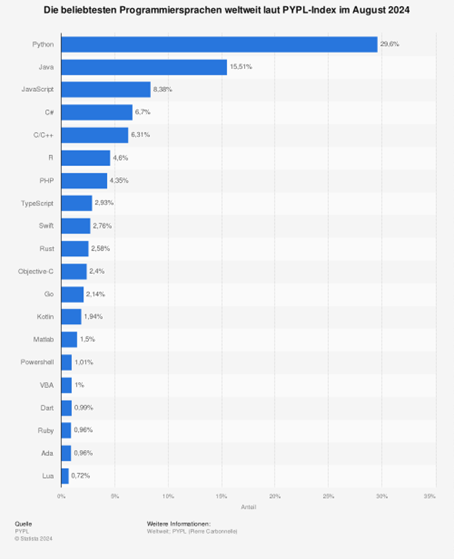
\includegraphics[width=0.7\linewidth]{images/Programmiersprachen.png}
	\caption[Programmiersprachen]{Programmiersprachen}
	\label{fig:Programmiersprachen}
\end{figure}

\subsection{Python}
Bei Python wird der Quellcode zur Laufzeit in Bytecode übersetzt und findet Anwendung in der Webentwicklung, Netzwerkprogrammierung sowie der Datenanalyse. Darüber hinaus wird diese Programmiersprache auch für die Automatisierung von Prozessen oder für Künstliche Intelligenz eingesetzt. \parencite{Programmiersprachen}


\textbf{Vorteile}
\begin{itemize}
	\item einfache Syntax
	\item kein manuelles Speichermanagement notwendig
	\item plattformunabhängiger Code
	\item stellt eine breite Auswahl an installierbaren Bibliotheken, Frameworks und umfassenden Support bereit
\end{itemize}

\textbf{Nachteile}
\begin{itemize}
	\item höherer Speicherbedarf
	\item für mobile Anwendungen gibt es nur eine begrenzte Unterstützung für die Entwicklungen
	\item langsamere Ausführungsgeschwindigkeit im Vergleich zu anderen Programmiersprachen
\end{itemize}

\subsection{Java}
Die umfangreiche Verbreitung und Beliebtheit von Java hat im Laufe der Zeit zu einer umfassenden Bibliothek geführt, die eine Vielzahl von Klassen und Funktionen für einige Anwendungsbereiche bereitstellt. Dies ermöglicht Entwicklern für häufig benötigte Lösungen auf bestehende Ressourcen zurückzugreifen und diese zu integrieren. \parencite{Programmiersprachen}

\textbf{Vorteile}
\begin{itemize}
	\item objektorientierte Programmierung, die eine klare Strukturierung und eine effektive Wiederverwendung von bestehendem Code ermöglicht
	\item Fehlererkennung und integrierte Sicherheitsmaßnahmen sorgen für hohe Sicherheit und Robustheit
	\item kein manuelles Speichermanagement erforderlich
	\item Skalierbarkeit unterstützt die Entwicklung großer und komplexer Anwendungen
\end{itemize}

\textbf{Nachteile}
\begin{itemize}
	\item längere Entwicklungs- und Einarbeitungszeiten aufgrund komplexer Strukturen und einer strikteren Syntax
	\item erhöhter Speicherbedarf
	\item mögliche Lizenzgebühren für die kommerzielle Nutzung
	\item fehlende Unterstützung bei Echtzeitanwendungen
\end{itemize}

\subsection{JavaScript}
JavaScript war ursprünglich eventbasiert - das heißt, der JavaScript - Code war so strukturiert, dass er auf Benutzerinteraktionen und Ereignisse reagiert, anstatt selbst aktiv zu werden. Diese Programmiersprache kommt heutzutage auch auf Servern und in Mikrocontrollern nicht nur in Webbrowsern zum Einsatz. \parencite{Programmiersprachen}

\textbf{Vorteile}
\begin{itemize}
	\item große Unterstützung von allen bekannten Webbrowsern
	\item plattformunabhängige Ausführung des Codes im Browser
	\item breite Community und eine weite Verbreitung
	\item leichte Erstellung interaktiver Webseiten und kleinerer Anwendungen
\end{itemize}

\textbf{Nachteile}
\begin{itemize}
	\item browserabhängige Interpretation des Codes ermöglicht es, dass es zu Abweichungen kommen kann und soll bei der Entwicklung beachtet werden
	\item geringere Performance im Vergleich zu anderen Programmiersprachen
	\item geringe Skalierbarkeit
\end{itemize}

\subsection{C\#}
C\# ist eine stark typisierte Programmiersprache, sie erfordert zwar einen größeren Aufwand, bietet aber eine verbesserte Fehlererkennung, was zu einer geringeren Anzahl an Bugs führt. Diese Programmiersprache ist speziell für die Entwicklung von Desktop-, Cloud-, Webanwendung, Spiele und mobilen Apps im Microsoft Umfeld ausgelegt. \parencite{Programmiersprachen}

\textbf{Vorteile}
\begin{itemize}
	\item dauerhafte Weiterentwicklung mit neuen Features
	\item große Community, die viele Tools und Unterstützungen anbieten
	\item Integration in die Microsoft Umgebung und deren verbundenen Ressourcen
	\item breites .NET-Framework mit großer Bibliothek und einigen Tools, sowie Funktionen
\end{itemize}

\textbf{Nachteile}
\begin{itemize}
	\item viele Konzepte und Funktionen, die aufwendig zum Erlernen sind
	\item eingeschränkte Plattformunabhängigkeit, deshalb eignet sich diese Programmiersprache hauptsächlich für Windows-Anwendungen
\end{itemize}

\subsection{C/C++}
Die Programmiersprache C ist eine der wenigen, die sich zum Programmieren von Betriebssystemen eignet. Weiters ist C bis heute der Standard für Betriebssysteme, Treiber und Embedded Systeme. Bei Embedded Systeme übernimmt der Computer Überwachungs-, Steuerungs-, Regelfunktionen oder ist für die Datenverarbeitung zuständig. C++ kombiniert die Vorteile der Kontrolle über die Hardware mit den Konzepten der objektorientierten Programmierung. Sie wird in Bereichen wie Spieleentwicklung über die Grafikprogrammierung bis hin zu Echtzeitsystemen zum Einsatz gebracht. \parencite{Programmiersprachen}

\textbf{Vorteile}
\begin{itemize}
	\item schnell und effizient durch die direkte Ausführung auf der CPU
	\item Hardware nahes Programmieren und der direkte Zugriff auf den Speicher ermöglichen manuelle Optimierungen
	\item großes Anwendungsgebiet und vielseitige Einsatzmöglichkeiten
	\item bietet durch C++ eine prozedurale als auch eine objektorientierte Programmierung
	\item sehr gute Skalierbarkeit
\end{itemize}

\textbf{Nachteile}
\begin{itemize}
	\item fehleranfällig aufgrund direkter Speicherkontrolle und -verwaltung
	\item schlechte Code könnte Sicherheitslücken eröffnen, wo sich Hacker Zugriff schaffen können
\end{itemize}



\subsection{Kotlin}
Kotlin wird für die Entwicklung von Android-Apps verwendet. Außerdem bietet diese Programmiersprache eine saubere und präzise Syntax im Vergleich zu Java. Zudem kann ein bestehender Java-Code problemlos in Kotlin Projekte integriert werden, dass selbe funktioniert auch umgekehrt. \parencite{Kotlin}

\textbf{Vorteile}
\begin{itemize}
	\item Sicherheit: durch die Unterstützung von immutablen Daten führt es zu wenigen Fehlern im Code
	\item Kotlin kann problemlos mit Java-Code und Bibliotheken zusammenarbeiten
	\item bietet eine moderne Syntax, die die Lesbarkeit und Wartbarkeit verbessert
\end{itemize}

\textbf{Nachteile}
\begin{itemize}
	\item weniger erfahrene Kotlin Entwickler als bei Java
	\item geringere Communitygröße
\end{itemize}


\section{Entwicklungsumgebungen}
Eine integrierte Entwicklungsumgebung ist eine Softwareanwendung, die alle Werkzeuge, die für ein Softwareentwicklungsprojekt benötigt werden, an einem Ort vereint. Einige IDEs sind auf eine spezifische Programmiersprache wie Python oder Java ausgerichtet. Die Mehrheit der IDEs ist jedoch so konzipiert, dass sie mit einer Vielzahl unterschiedlicher Programmiersprachen kompatibel ist. Die bekanntesten Anbieter von integrierten Entwicklungsumgebungen sind Visual Studio, IntelliJ IDEA, Microsoft, JetBrains. 

\subsection{Funktionen von IDEs}
Alle integrierten Entwicklungsumgebungen beinhalten einen Texteditor, der die Erstellung und Bearbeitung von Quellcode ermöglicht. Darüber hinaus bieten einige IDEs visuelle Komponenten und Drag-and-Drop-Schnittstellen für die Entwicklung von Frontend-Komponenten an. Üblicherweise sind diese Editoren mit einer Syntaxhervorhebung ausgestattet, um die Lesbarkeit und Fehlererkennung im Code zu erleichtern. Debugging-Tools unterstützen Anwender bei der Behebung von Fehlern im Quellcode. Profiling ermöglicht die Analyse von Laufzeit, CPU-Auslastung von Programmen und Speicherverbrauch, um Leistungsengpässe sowie Optimierungspotenziale durch eine Visualisierung von Daten zu identifizieren. 

\subsection{Arten von IDEs}
\textbf{Mehrsprachige integrierte Entwicklungsumgebungen} sind mit einer Vielzahl von Programmiersprachen kompatibel. Zu den bekanntesten gehört Visual Studio, das für seine umfangreichen Funktionen und regelmäßigen Updates geschätzt wird. Die Unterstützung für zusätzliche Programmiersprachen kann durch die Installation von Erweiterungen integriert werden. Mit dem Aufkommen der mobilen App-Entwicklung haben sich spezialisierte IDEs für diesen Bereich etabliert. Diese Plattformen ermöglichen Entwicklern die Erstellung effizienter und umfassender mobiler Anwendungen. Beispiele hierfür sind Android Studio für die Android-Entwicklung und Xcode für die iOS-Entwicklung.

Gegenüber lokalen Entwicklungsumgebungen bieten \textbf{Web- oder Cloud basierte IDEs} mehrere Vorteile. Eine SaaS-IDE (Software as a Service) ermöglicht es, Aufgaben auszuführen, ohne die Ressourcen einer lokalen Workstation zu belasten. Diese cloudbasierten IDEs sind oft plattformunabhängig und können nahtlos mit verschiedenen Cloud-Anbietern integriert werden.
Sprachspezifische IDEs hingegen richten sich an Entwickler, die ausschließlich mit einer einzigen Programmiersprache arbeiten möchten. Beispiele hierfür sind Jikes und Jcreator für Java, CodeLite und C-Free für C/C++, sowie Idle für Python. \parencite{integrierteEntwicklungsumgebung}



\section{Vergleich Single Board Computer und Mikrocontrollern}
\subsection{Single Board Computer}
Einplatinencomputer (Single-Board Computers, SBCs) sind Computersysteme, bei denen sämtliche notwendigen Komponenten, wie Prozessor, Speicher und Ein-/Ausgabeschnittstellen, auf einer einzigen Platine integriert sind. Diese Geräte fungieren oft als Hauptprozessor in eingebetteten Systemen oder werden als kostengünstige Allzweckcomputer eingesetzt.

\textbf{Vorteile}
\begin{itemize}
	\item kompakte Bauweise
	\item geringes Gewicht
	\item flexible Einsatzmöglichkeit
	\item reduzierten Energieverbrauch 
	\item niedrige Kosten
	\item benutzerfreundlich
	\item erfordern minimale Vorbereitungen für den Betrieb
\end{itemize}

\textbf{Nachteile}
\begin{itemize}
	\item hohe Kosten, da sie viele Funktionen und Komponenten beinhalten
	\item größer und schwerer als Mikrocontroller
	\item hoher Stromverbrauch
\end{itemize}

\subsubsection{Arten von SBCs}
Einplatinencomputer lassen sich in drei Hauptkategorien unterteilen: einem Mikrocontroller basierten, einem Mikroprozessor basierten und einem FPGA basierten System. 

Die einfachste und kostengünstigste Art ist ein \textbf{Mikrocontroller basierter Einplatinencomputer}. Mikrocontroller-basierte SBCs zeichnen sich in der Regel durch einen einzigen Mikrocontroller-Chips aus, der alle grundlegenden Funktionen des Systems übernimmt, einschließlich Ein- und Ausgabe, Speicher und Energieverwaltung. 

Im Gegensatz dazu verfügen \textbf{mikroprozessorbasierte SBCs} über einen Mikroprozessor anstelle eines Mikrocontrollers, was eine höhere Leistungsfähigkeit verleiht. Mikroprozessoren sind vielfältiger und in der Lage, anspruchsvollere Aufgaben zu bewältigen. 

Die leistungsstärkste Kategorie von SBCs sind \textbf{FPGA-basierte Systeme}, die mit einem Field-Programmable Gate Array (FPGA) ausgestattet sind. FPGAs sind vielseitige Chips, die so programmiert werden können, dass sie verschiedene Arten von Logikchips nachbilden, einschließlich Mikroprozessoren oder Mikrocontrollern, und damit eine hohe Flexibilität und Leistungsfähigkeit bieten.

\subsubsection{Typen von SBCs}
Es existieren verschiedene Typen von Einplatinencomputern. Der Raspberry Pi ist ein weit verbreiteter, kostengünstiger Singleboard Computer. Weitere leistungsstärkere Modelle umfassen den BeagleBone und die Odroid-Serie, die ebenfalls breite Anwendung finden.

\subsubsection{Betriebssysteme für SBCs}
Die meisten SBCs laufen mit Linux-basierten Betriebssystemen wie Raspbian, Ubuntu oder Fedora. Daneben können auch andere Betriebssysteme wie Windows 10 IoT Core und Android auf SBCs verwendet werden. \parencite{EinplatinencomputerSBCs}

\begin{figure}[H]
	\centering
	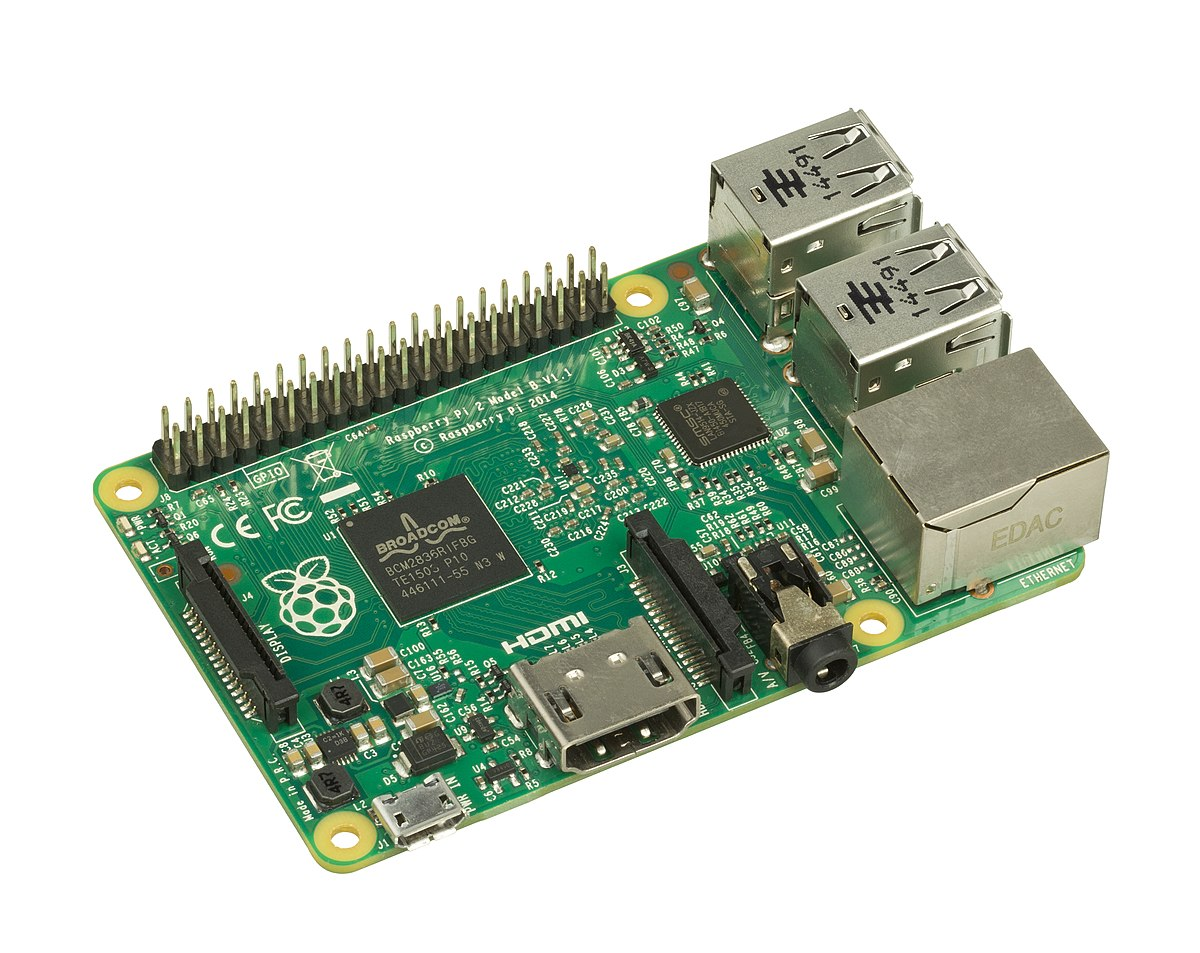
\includegraphics[width=0.7\linewidth]{images/SingleBoard Computer.jpg}
	\caption[Single Board Computer]{Single Board Computer}
	\label{fig:Single Board Computer}
\end{figure}

\subsection{Mikrocontroller}
Sind kleine Computer-Systeme, die für eine begrenzte Anzahl von Aufgaben entwickelt wurden. Mikrocontroller enthalten einen Prozessor, Speicher und I/O-Ports. Häufig werden sie für einfachere Anwendungen wie die Steuerung von Geräten und Maschinen verwendet. \parencite{EinzelplatinencomputerVsMikrocontroller}

\textbf{Vorteile}
\begin{itemize}
	\item kosteneffizienter als SBCs
	\item geringer Stromverbrauch
	\item klein und leicht, geeignet für Projekte wo man tragbare Geräte benötigt 
\end{itemize}

\textbf{Nachteile}
\begin{itemize}
	\item keine Netzwerkfähigkeiten oder Anschlüsse für externe Geräte
	\item beschränkte Funktionalitäten, komplexere Aufgaben können teilweise nicht ausgeführt werden
\end{itemize}

\begin{figure}[H]
	\centering
	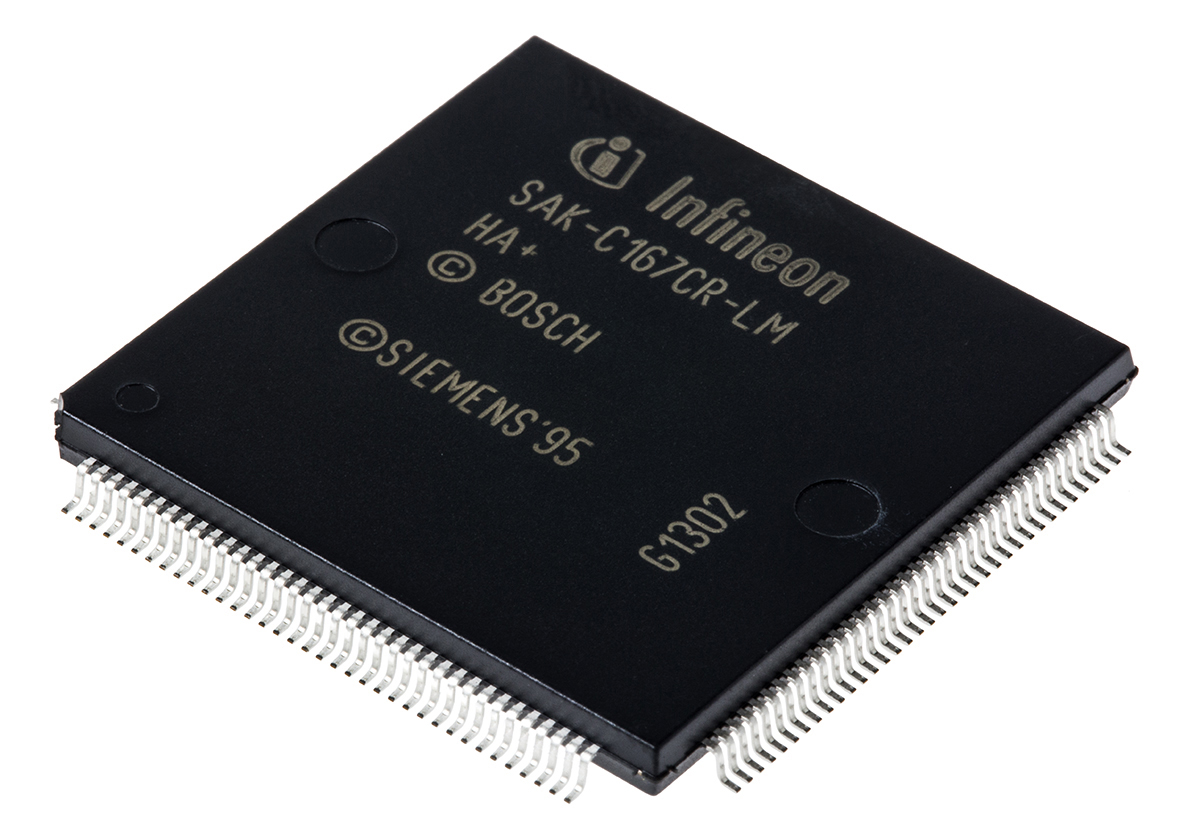
\includegraphics[width=0.7\linewidth]{images/Mikrocontroller.jpg}
	\caption[Mikrocontroller]{Mikrocontroller}
	\label{fig:Mikrocontroller}
\end{figure}


\section{Vergleich von GitHub und GitLab}
\subsection{GitHub}
GitHub ist eine Cloud-basierte Plattform, auf der Code gespeichert, sowie geteilt wird und man mit anderen Personen zusammenarbeiten kann. Dateien werden in GitHub hochgeladen und in einem Repository gespeichert. Bei Änderungen der Dateien wird GitHub automatisch beginnen die Änderungen nachzuverfolgen und zu verwalten. Sobald mehrere Personen an einem Repository zusammenarbeiten, müssen die Änderungen von allen Mitarbeitern auf GitHub abgerufen, sowie die eigenen Änderungen an das Repository auf GitHub gepusht werden. \parencite{GitHubUndGit}

\textbf{Vorteile}
\begin{itemize}
	\item die Arbeit leicht präsentieren oder teilen
	\item Änderungen des Codes jederzeit nachverfolgen, sowie verwalten
	\item an einem Projekt zusammenarbeiten ohne, dass sich die Änderungen auf die Arbeit der Mitarbeiter auswirkt
	\item kostenloser Service
	\item große Community
\end{itemize}

\textbf{Nachteile}
\begin{itemize}
	\item Speicherplatzbeschränkungen, da 100MB in einer Datei nicht überschritten werden können
	\item Repositories sind in der kostenlosen Version auf 1GB beschränkt
\end{itemize}


\begin{figure}[H]
	\centering
	\includegraphics[width=0.5\linewidth]{images/GitHub.png}
	\caption[GitHub]{GitHub}
	\label{fig:GitHub}
\end{figure}

\section{GitLab}
GitLab ist eine Alternative zu GitHub und wurde entwickelt, um Open Source Projekte zu hosten. Hosting für Wikis und Burg-Tracking Systeme werden angeboten und Berechtigungen für verschiedene Mitarbeiter können entsprechend ihrer Rolle festgelegt als auch geändert werden. Weiters kann man bei GitLab die eigenen Repos kostenlos hosten. GitLab bietet einige sehr interessante Funktionen und ist mittlerweile sehr beliebt geworden.   \parencite{GitHubVsGitLab}

\textbf{Vorteile}
\begin{itemize}
	\item ist eine Open Source Lizenz
	\item gut in Git integriert
	\item ermöglicht Self Hosting
\end{itemize}

\textbf{Nachteile}
\begin{itemize}
	\item Benutzeroberfläche ist langsamer als bei GitHub
	\item häufig Probleme bei Repositories 
\end{itemize}


\begin{figure}[H]
	\centering
	
\includegraphics[width=0.5\linewidth]{images/GitLab.png}
	\caption[GitLab]{GitLab}
	\label{fig:GitLab}
\end{figure}

Für StageControl wird GitHub verwendet, da es zahlreiche Vorteile bietet, wie oben genannt, und die Zusammenarbeit im Team erleichtert. So können mehrere Personen gleichzeitig an Unterschiedlichen Aspekten arbeiten, ohne dass sich ihre Änderungen gegenseitig beeinflussen.

\section{SD-Karten Sicherung}
Eine SD-Karte ist eine kleine Speicherkarten, die in einigen tragbaren Geräten verwendet wird, wie zum Beispiel in Android Handys, Navi Systeme in einem Auto oder Digitalkameras. Es ist wichtig eine SD-Karte zu sichern, da die Daten aufgrund von pysischen Schäden an der SD-Karte oder Mailwareangriffen verloren gehen könnten. Wenn die Daten der SD-Karte verloren gehen, wäre ein Backup hilfreich, um diese verlorenen Daten wieder herzustellen.  \parencite{SD-KartenSicherung}

\subsection{Sicherungskopie einer SD-Karte}
Eine Sicherungskopie wird vorgenommen, wenn nur kleine Daten von einer SD-Karte zum Sichern sind. Hierbei wird der SD-Kartenleser an den Computer angeschlossen und die Datei auf das Laufwerk des Computers kopiert. Doch um größere Dateien zu sichern, reicht diese Methode nicht aus. \parencite{SD-KartenSicherung}

\subsection{Klonen einer SD-Karte}
Hierbei wird eine identische Kopie des Quelllaufwerks erstellt und alle Inhalte der SD-Karte werden auf das Ziellaufwerk kopiert. Die am häufigsten verwendete Programme dafür sind Win32 Disk Imager und Balena Etcher. \parencite{SD-KartenSicherung}

\subsection{Vergleich von Win32 Disk Imager und Balena Etcher}
Beide Programme sind kostenlos nutzbar und sind Open-Source Anwendungen. Sie sind beide einfach zu bedienen. Bei der Benutzerfreundlichkeit sind beide Programme ident, sowie die Schritte zum Sichern der SD-Karte. Balena Etcher und Win32 Disk Imager können beide Image-Dateien auf USB Flash Laufwerke, SD-Karten und Wechseldatenträger schreiben. Der Unterschied von den zwei Programmen liegt darin, dass Win32 Disk Imager die SD-Karten oder USB-Sticks wiederherstellen kann. \parencite{VergleichvonWin32DiskImagerundBalenaEtcher}

\section{Peer to Peer Netzwerk}
Ein Peer to Peer Netzwerk wird auch als \textit{"Kommunikation unter Gleichen"} bezeichnet und ist ein Netzwerk in welchem alle Rechner die gleichen Funktionen beinhalten. Wenn innerhalb eines Peer to Peer Netzwerks eine Datei heruntergeladen werden möchte, wird an alle Computer im Netzwerk eine Anfrage gesendet. Diese Computer beziehungsweise Peers stellen diese Datei zur Verfügung, somit werden die einzelnen Teile von unterschiedlichen Peers heruntergeladen. Doch die bereits erhaltenen Teile werden bereitgestellt, sodass die anderen Nutzerinnen und Nutzer die Datei von ihrem Computer auch erhalten können. \parencite{PeertoPeerNetzwerk}

Das Peer to Peer Netzwerk bietet Vorteile, als auch Nachteile. 

\textbf{Vorteile}
\begin{itemize}
	\item Skalierbar, je mehr Computer, desto leistungsstärker ist es
	\item sicher, da es meistens keinen Hauptserver gibt
	\item flexiblere Aufgabenverteilung im Netzwerk 
\end{itemize}

\textbf{Nachteile}
\begin{itemize}
	\item aufwendige Verwaltung und Organisation eines großen Peer to Peer Netzwerkes 
	\item Abhängigkeit von anderen Computer im Netzwerk
\end{itemize}

\section{Corporate Identity}
Die Corporate Identity ist das wichtigste Merkmal, das ein Unternehmen kennzeichnet und von anderen unterscheidet. Die Corporate Identity wird in drei Teilbereiche unterteilt, welches in der Abbildung \ref{fig:CorporateIdentity} zu sehen ist:

\begin{figure}[H]
	\centering
	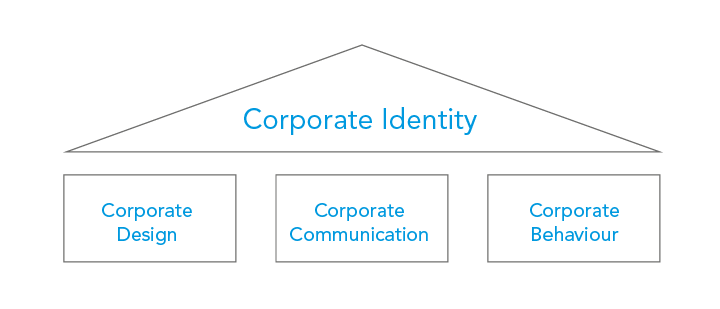
\includegraphics[width=0.5\linewidth]{images/CorporateIdentity.png}
	\caption[Corporate Identity]{Corporate Identity}
	\label{fig:CorporateIdentity}
\end{figure}

\subsection{Corporate Design}
Das Corporate Design beschreibt das interne und externe Erscheinungsbild eines Unternehmens. Hierzu zählen die Farben, Schriften und das Logo, die das Unternehmen einheitlich präsentieren. \parencite{CorporateIdentity}

\subsubsection{Logo}
Das Logo ist eines der wichtigsten Bestandteile da es einen Wiedererkennungswert des Unternehmens hat. Das Unternehmenslogo soll auf die Tätigkeit und die Farben des Unternehmens hinweisen. Es soll einfach aufgebaut  und einprägsam sein. Darüber hinaus sollte das Logo so entworfen sein, sodass es auf den verschiedensten Werbemitteln dargestellt werden kann. Es gibt drei verschiedene Arten von einem Logo: Wortmarke, Bildmarke oder Kombinierte Marke. Wortmarken bestehen auf Buchstaben oder Zahlen. Hingegen eine Bildmarke nur aus einem Bild oder Zeichen besteht. Die Kombinierte Marke oder auch Wort-Bild-Marke genannt, ist eine Mischung aus Wortmarke und Bildmarke. \parencite{Firmenlogo} 

In der Abbildung \ref{fig:Beispiele für Wortmarke, Bildmarke, Kombinierte Marke} sind Beispiele von den drei verschiedenen Arten eines Logos zu sehen.

\begin{figure}[H]
	\centering
	\includegraphics[width=0.5\linewidth]{images/Beispiele für Wortmarke, Bildmarke, Kombinierte Marke.jpg}
	\caption[Beispiele für Wortmarke, Bildmarke, Kombinierte Marke]{Beispiele für Wortmarke, Bildmarke, Kombinierte Marke}
	\label{fig:Beispiele für Wortmarke, Bildmarke, Kombinierte Marke}\parencite{Logodesign}
\end{figure}

\subsubsection{Unternehmensfarben}
Die Unternehmensfarben und das Logo repräsentieren das Unternehmen nach innen und außen. Farbtöne strahlen unterschiedliche Wahrnehmnungen aus. Es beeinflusst wie die Marke auf den Kunden wirkt und wie sich das Unternehmen von der Konkurrenz abhebt. \parencite{Unternehmensfarbe}

\subsubsection{Unternehmensschrift}
Die Unternehemnsschrift ist zwar ein Teil des Erscheinungsbilds, jedoch ist dieser Teil nicht so wichtig. Es können bestehende Schriften, aber auch eine neue Schrift verwendet werden. Innerhalb des Unternehmens sollte jedoch eine Schriftart für alle Werbemittel oder Medien festgelegt werden. Die Schriftart sollte gut leserlich sein und zu dem Produkt oder der Tätigkeit passen. \parencite{Unternehmensschrift}

\subsection{Corporate Communication}
Die Corporate Communication vermittelt die Unternehmensidentität durch eine einheitliche Kommunikation nach innen und außen. Die Kommunikation inner- und außerhalb des Unternehmens wirkt sich auf die Betriebsatmosphäre aus. Dies wird durch einen Slogan wiedergegeben.

\subsection{Corporate Behaviour}
Das Corporate Behaviour beschäftigt sich mit dem Benehmen und dem Umgang der Mitarbeiter, sowie der Führungskraft. Es sollte ein einheitliches Gesamtbild, sowie angenehmes Arbeitsklima im Unternehmen geschaffen werden. 

\section{Adobe Programme}
Für die Umsetzung vom Logo, Flyer und der Animation wurden einige Programme verwendet. Diese werden wie folgt erläutert.

\subsection{Adobe Indesign}
Adobe Indesign ist ein Programm, welches zum Designen von Printmedien, wie Broschüren und Flyer dient.
Die Verwendung von Adobe Indesign ermöglicht Stage Control, die Gestaltung vom Flyer. Das Programm stellt eine breite Auswahl von Werkzeugen und Funktionen dar. Weiters können verschiedene Schriftarten und Textformate eingesetzt werden, womit sich die Lesbarkeit verbessert. Darüber hinaus kann das Layout auf die verschiedensten Seitenformate optimiert werden. Mithilfe von der Absatz- und Zeichenformatfunktion kann eine durchgehenede Formatierung sichergestellt werden. \parencite{AdobeIndesign}

Zusammenfassend ist Adobe Indesign ein sehr leistungsstarkes Programm mit zahlreichen Funktionen. Es ermöglicht hochwertiges Werbematerial für StageControl zu erstellen.

\subsection{Adobe Illustrator}
Adobe Illustrator wird oft für Vektorgrafiken verwendet. Mit diesem Programm werden Logos, Grafiken und Illustrationen erstellt. Die Grafiken bestehen aus Punkten, Linen und Kurven anstatt aus Pixeln, deshalb werden diese in jeder Größe scharf angezeigt. Mithilfe des Formerstellungswerkzeug können komplexere Formen kreiert werden, sowie auch 3D Abbildungen oder Farbverläufe. \parencite{AdobeIllustrator}

Insgesamt ist Adobe Illustrator ein praktisches Programm, dass das Erstellen von Logos, Grafiken und Illustrationen vereinfacht. Es ermöglicht ein qualitativ hochwertiges Logo zu gestalten. Im Rahmen der Diplomarbeit von Stage Control wird Adobe Illustrator für die Erstellung vom Logo verwendet. 

\subsection{Adobe After Effects}
Adobe After Effects wird für Motion Design, Animationen und visuelle Effekte verwendet. Mit diesem Programm werden Text und Grafiken animiert um visuelle Inhalte zu kreiren. Mit den Kompositionen \textit{(Rahmen für ein Video, der aus verschiedenen Ebenen besteht)} werden Special Effects für Film, TV oder Video erstellt. Adobe After Effects bietet ebenfalls einige Funktionen und Werkzeuge an. Somit können die verschiedenen Inhalte der Animation, wie Schrift, Farben und Grafiken angepasst werden. \parencite{AdobeAfterEffects}

Alles in allem bietet Adobe After Effects einige Funktionen, die es ermöglicht eine hochwertige Animation zu erstellen. Diese wird in dem Werbeclip verwendet. 

\chapter{Ergebnisdokumentation}
\section{Einleitung}
\subsection{Was ist StageControl?}
StageControl ist eine GUI-App für die Indoor-Navigation auf einer Bühne. Sie verwendet ESP32 UWB Sensoren und Trilateration, um den Standort des Musikers zu bestimmen. Mit einer grafischen Darstellung des Standortes bietet StageControl eine benutzerfreundliche Erfahrung. Wichtig zu betonen ist, dass die App derzeit noch als Proof-of-Concept des System dient und kein fertiges Projekt darstellt. 

\subsection{Themenabgrenzung}
StageControl ist eine neue Idee. Es existiert nach unserer Recherche keine Anwendungen wie StageControl. StageControl bezweckt eine technische Indoor-Navigation auf einer Bühne mit GUI-Visualisierung. 

\subsection{Entwicklungsprozesse}
Die Umsetzung der Diplomarbeit StageControl folgt nach dem Wasserfall-Modell. Dieses Modell besagt, dass die Arbeitspakete im Vorfeld geplant werden und durchgeführt werden. Dadurch kann die Zuweisung von Aufgaben an die Teammitglieder unabhängig durchgeführt werden. 

Um den Programmcode für die App und alles weitere fortlaufend zu dokumentieren, wird das Versionskontrollsystem GitHub verwendet. 

\section{Entwicklung}
Die Entwicklung wurde mit folgenden Programmen \& Programmiersprachen umgesetzt.

\textbf{Arduino IDE} \ – IDE für ESP32 UWB Entwicklung \\
\textbf{IntelliJ IDEA} \ – IDE für Entwicklung des GUI \\
\textbf{Java} \ – Programmiersprache für GUI \\
\textbf{FXML} \ – Auszeichnungssprache für die Szenen der GUI \\
\textbf{C++} \ – Programmiersprache für ESP32 UWB \\
\textbf{PostgreSQL} \ – Datenbank \\
\textbf{VMware Workstation Pro} \ - Virtuelle Maschine

\subsection{JavaFX statt Android Studio}
Anfangs war geplant mit Android Studio und Kotlin eine App zu entwickeln. Diese Idee haben wir aufgrund von diversen Gründen (Kompatibilität, Plattformübergreifende UIs, Neuerlernung, usw.) verworfen. Da sich JavaFX besonders für die Desktop-Entwicklung eignet haben wir uns schlussendlich dafür entschieden.

\section{Verschiedene Arten von UWB Sensoren}

Es gibt verschiedene Arten von ESP32 UWB Modulen mit denen wir uns beschäftigt haben:

\begin{table}[h]
	\centering
	\small
	\begin{tabular}{|l|c|c|c|}
		\hline
		\textbf{Feature} & \textbf{UWB Pro} & \textbf{UWB Pro with Display} & \textbf{UWB DW3000} \\
		\hline
		CPU & ESP32-WROVER & ESP32-WROVER & ESP32-WROOM/WROVER \\
		\hline
		Core UWB & DW1000 & DW1000 & DW3000 \\
		\hline
		Screen & N & Y & N \\
		\hline
		Measuring Distance (m) & 200 & 200 & 20 \\
		\hline
		Battery Socket & N & Y & N \\
		\hline
		UWB Channel & 2/5 & 2/5 & 5/9 \\
		\hline
		Apple Interoperable & N & N & Y \\
		\hline
		Suitable for & Long distance needed & Long distance needed & Product development \\
		\hline
	\end{tabular}
	\caption{Comparison of UWB Modules}
	\label{tab:uwb_comparison}
	\parencite{ArtenSensorn}
\end{table}

\subsection{ESP32 mit MPU-6050}
Die Grundidee war es mit Hilfe eines Beschleunigungssensor (MPU-6050) die genau Position über Trägheitsnavigation zu ermitteln. Dabei ist bei der Berechnung außerdem zu beachten, dass man die Erdbeschleunigung wegrechnen muss. Der MPU-6050 liefert Beschleunigungsdaten, diese müssten zu Positionsdaten umgerechnet werden, was schlussendlich nicht ohne diverese und unerklärlichen Fehlerakkumulation führte. Deshalb wurde diese Idee verworfen und wir sind mit der UWB-Technolgie fortgefahren. \parencite{MPU6050}

\subsection{ESP32 UWB Pro}

Der ESP32 wurde bereits in 2.9.2 thematisiert. Wichtig ist aber zu sagen, dass wir einen ESP32 mit UWB (=Ultrawideband) Funktion und der DW1000Ranging Bibliothek verwendet haben, um uns die Distanzen zwischen Anchor und Tag angeben lassen können. Diese Module unterscheiden sich wie folgt:

\textbf{Tag}

Um einen Tag zu initialisieren, muss im Code folgende Zeile hinzugefügt werden.
\begin{lstlisting}[style=C++, caption=Tag Initialisierung, captionpos=b]
	#define TAG_ADD "7D:00:22:EA:82:60:3B:9C"
	DW1000Ranging.startAsTag(TAG_ADD, DW1000.MODE_LONGDATA_RANGE_LOWPOWER);
\end{lstlisting}  

\textbf{Anchor}

Um einen Anchor zu initialisieren, muss im Code folgende Zeile hinzugefügt werden.
\begin{lstlisting}[style=C++, caption=Anchor Initialisierung, captionpos=b]
	#define ANCHOR_ADD "86:17:5B:D5:A9:9A:E2:9C"
	DW1000Ranging.startAsAnchor(ANCHOR_ADD, DW1000.MODE_LONGDATA_RANGE_LOWPOWER, false);
\end{lstlisting} 

Die Funktion \textit{.startAsAnchor} erhält die folgenden Parameter: den Modus – in unserem Fall \textit{LONGDATA\textunderscore RANGE\textunderscore LOWPOWER} – sowie den Boolean-Wert \textit{false}. Dieser Wert bedeutet, dass keine zufällige Kurzadresse zugewiesen wird, sodass der Tag erkennen kann, welcher Anchor es ist.

Dieser Modi ist jedoch der einzige, welcher die richtigen Abstandwerte zwischen Anchor und Tag liefert, deshalb haben wir uns dafür entschieden.

Wichtig zu beachten ist, dass der Tag einen ähnlichen Code verwendet. Allerdings bleibt der Parameter für die Kurzadresse leer, um Verbindungsprobleme zu vermeiden. Der Modus muss dabei identisch sein.

\textbf{UWB}

UWB steht für Ultrawideband und ist eine Funktechnologie aus den 1960er Jahren. Diese Art von Kommunikationstechnologie ist darauf spezialisiert superschnell kurze Distanzen auszutauschen. Die hohe Präzesion kann bis auf wenige Zentimeter genau verwendert werden. \parencite{UWB}

\textbf{Pinbelegung}

Zu beachten ist, dass die Pinbelegung wichtig ist, die Module kommunizieren über diese und müssen, sowohl beim Anchor als auch Tag Modul gleich belegt werden. Außerdem ist zu betonen, dass jedes Modul, egal ob Anchor oder Tag eine eindeutige und einzigartige ID benötigt, um im System zu funktionieren.Um die Mikrocontroller zu programmieren, wurde als IDE Arduino verwendet, die Programmiersprache ist C++.

\textbf{Anchor:}
\begin{lstlisting}[style=C++, caption=Pinbelegung für Anchor, captionpos=b]
	#define SPI_SCK 18
	#define SPI_MISO 19
	#define SPI_MOSI 23
	
	#define UWB_SS 21
	#define UWB_RST 27
	#define UWB_IRQ 34 
	
	#define I2C_SDA 4
	#define I2C_SCL 5
\end{lstlisting}


\textbf{Tag:}
\begin{lstlisting}[style=C++, caption=Pinbelegung für Tag, captionpos=b]
	#define SPI_SCK 18
	#define SPI_MISO 19
	#define SPI_MOSI 23
	
	#define UWB_SS 21
	#define UWB_RST 27
	#define UWB_IRQ 34 
	
	#define I2C_SDA 4
	#define I2C_SCL 5
\end{lstlisting}

\section{Arduino Entwicklung}
Um Mikrocontroller ansprechen und programmieren zu können, muss man sich für eine IDE entscheiden, hierbei ist die Arduino IDE, \textcite{Arduino}
die Bekannteste und Einfachste.

Um ein ESP32 zu verwenden, muss man die vom Hersteller Espressif bereitgestellte Bibliothek \texttt{Arduino\_ESP32\_OTA} installieren. Anschließend verbindet man den Mikrocontroller mit einem USB-C-Kabel mit dem Computer. In der Arduino IDE kann man den ESP32 dann auswählen und Code auf den Mikrocontroller übertragen.

\begin{figure}[H]
	\centering
	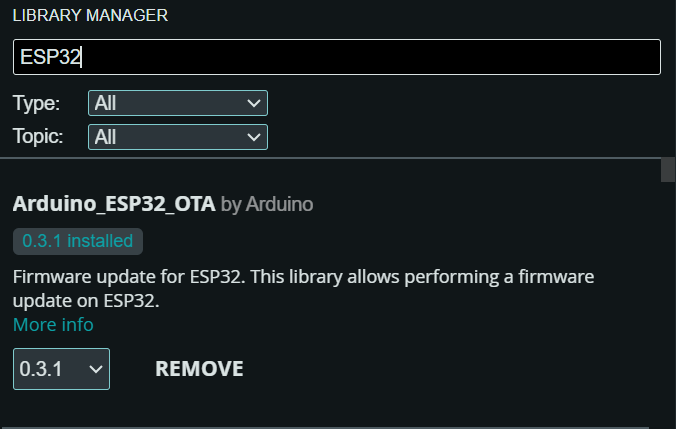
\includegraphics[width=0.5\linewidth]{images/ArduinoLib.png}
	\caption[ESP32Library]{ESP32 Library}
	\label{fig:ESP32Lib}
\end{figure}

\subsection{Arduino Bibliotheken}
Um den ESP32 zu compilen, die Funktion von UWB und andere Funktionen zu verwenden, muss man Biblotheken im Code verwenden: 
\begin{lstlisting}[style=C++, caption=Biblotheken, captionpos=b]
	#include <SPI.h>
	#include "DW1000Ranging.h"
	#include "DW1000.h"
	#include <Wire.h>
	#include <Adafruit_GFX.h>
	#include <Adafruit_SSD1306.h>
\end{lstlisting}

\textbf{\texttt{SPI.h}} \ – Standardbibliothek für die SPI-Kommunikation (Serial Peripheral Interface) \\
\textbf{\texttt{DW1000Ranging.h}} \& \textbf{\texttt{DW1000.h}} \ – Bibliotheken für UWB-Technologie (Ultra-Wideband) zur Entfernungsmessung \\
\textbf{\texttt{Wire.h}} \ – Bibliothek für I2C-Kommunikation \\
\textbf{\texttt{Adafruit\_GFX.h}} \& \textbf{\texttt{Adafruit\_SSD1306.h}} \ – Bibliotheken zur Steuerung eines OLED-Displays mit SSD1306-Treiber



\section{Setup des Projektes}
In diesem Abschnitt wird das Setup des Projektes, also Bühneneinrichtung, Kalibrierung, usw. thematisiert.

\subsection{Anchor \& Tag Setup}
Um das Setup zu starten, muss man auf einige Dichte achten (Aufstellung der Anchors siehe Grafik \ref{fig:AnchorTagSetup}, siehe \ref{Einrichtung Bühne} Einrichtung der Bühne, siehe \ref{KalibrierungDerAnchor} Kalibrierung der Anchor). In nachfolgender Grafik ist das grundlegende Setup dargestellt.

\begin{figure}[H]
	\centering
	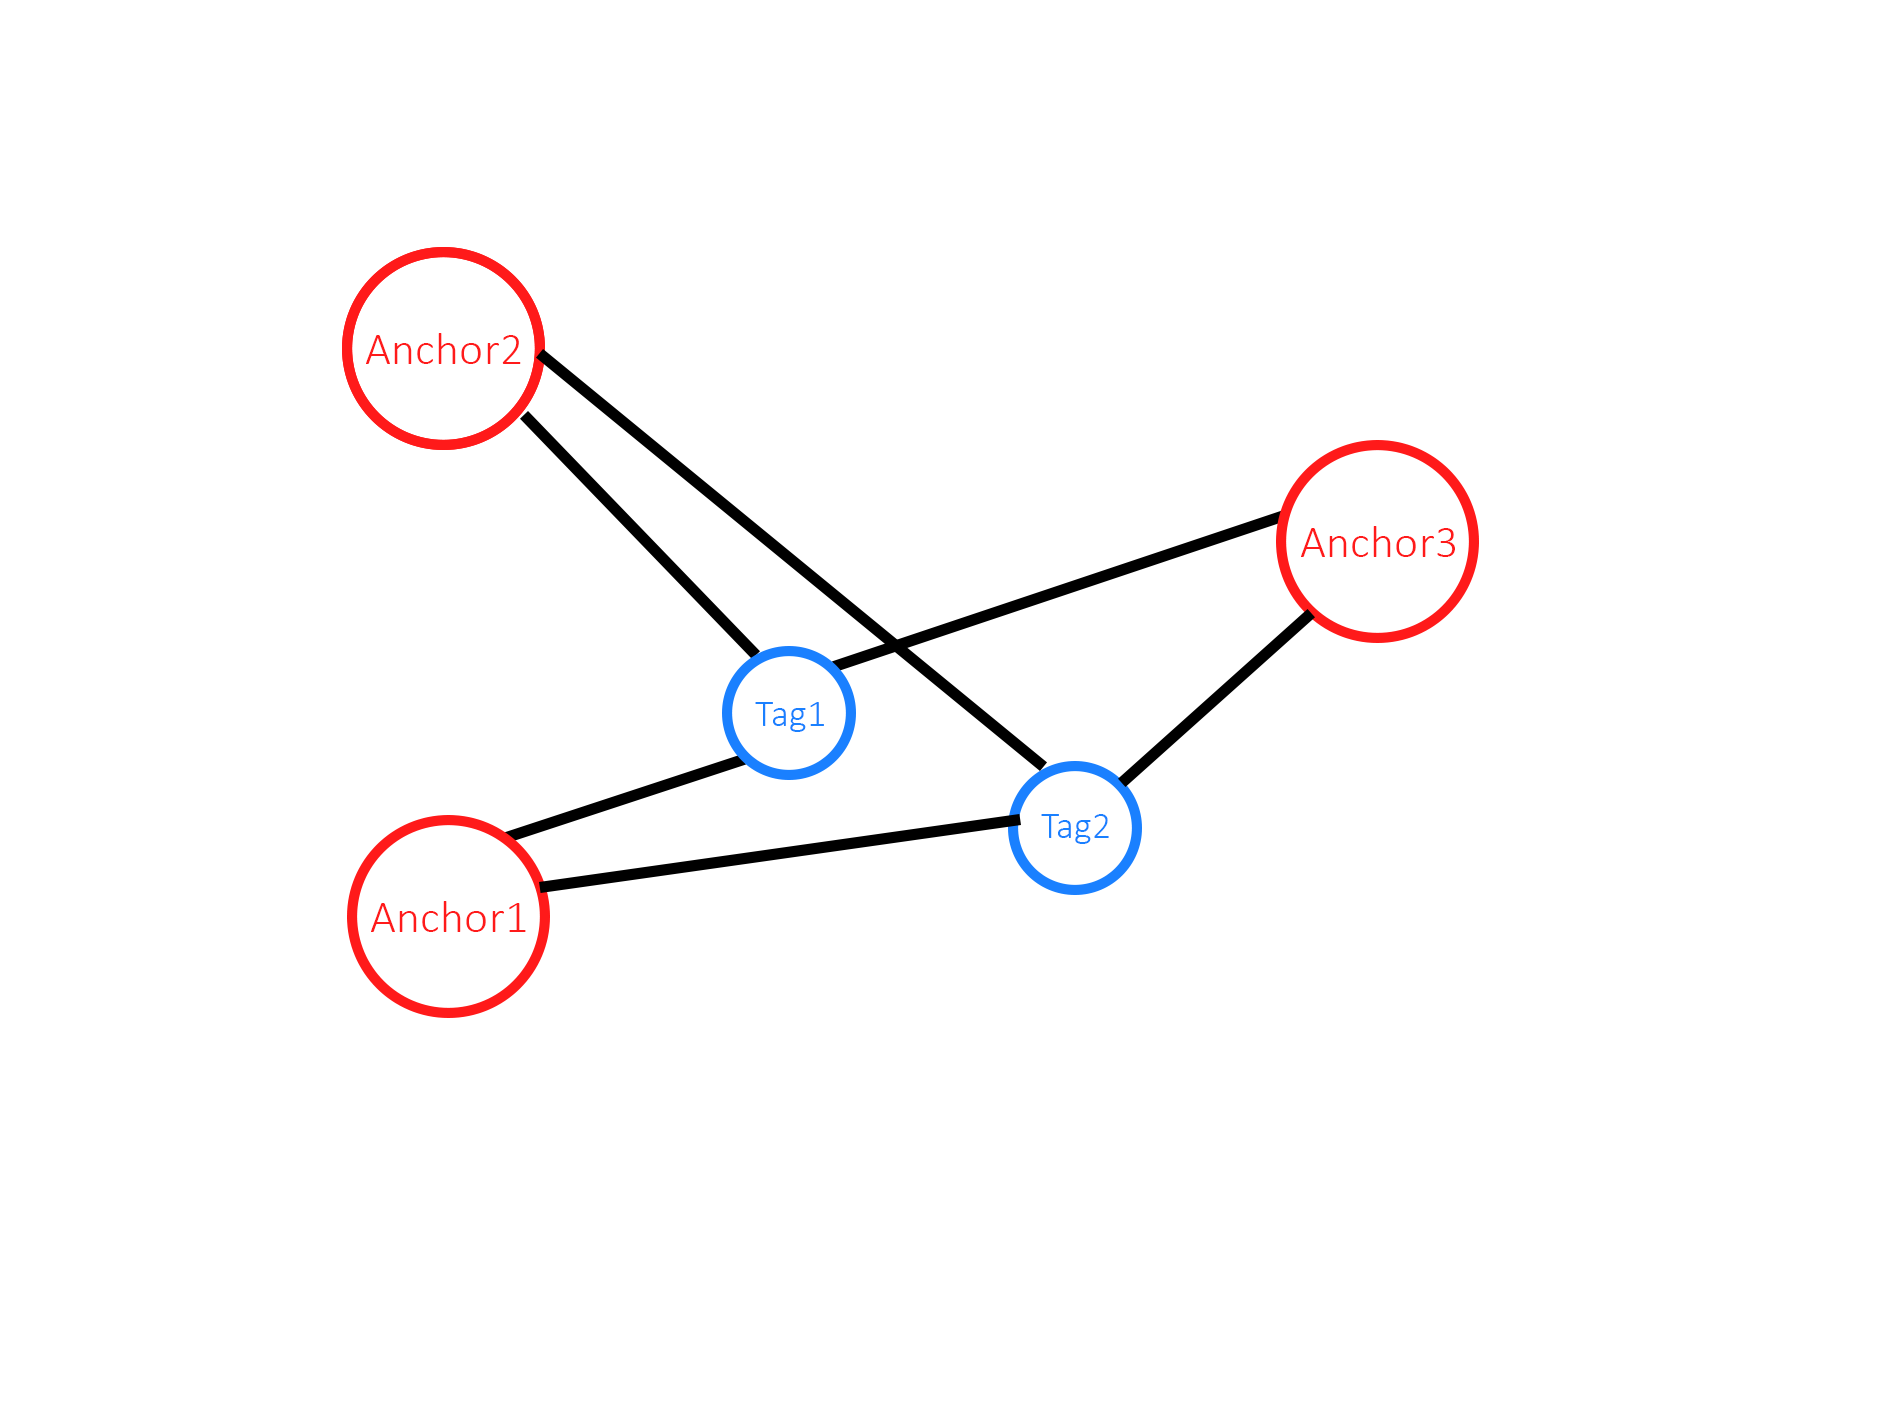
\includegraphics[width=0.5\linewidth]{images/AnchorTagSetup.png}
	\caption[AnchorTagSetup]{Anchor \& Tag Setup}
	\label{fig:AnchorTagSetup}
\end{figure}

Die roten Kreise stellen die Anchors dar, welche immer in einem Dreieck platziert werden müssen. Die blauen Kreise sind die Tags, welche beliebig hinzugefügt werden können. Die schwarzen Linien sind die Abstände zwischen den Tags und den Anchors, diese werden für die Trilateration benötigt, diese werden für die genaue Bestimmung auf der Bühne benötigt. 

\subsection{Kalibrierung der Anchor}
\label{KalibrierungDerAnchor}
Die Kalibrierung erfolgt im Code des jeweiligen Anchors. Dieser erstellt einen Mittelwert aus vier rohen Rangedaten und sendet diese dann an den Tag, welcher wiederum die Daten an das GUI für die Berechnung schickt. In unserem Fall gehen wir immer von Werten zwischen 0,5 und 50,0m aus, diese können, aber im Code variable verändert werden.

\begin{lstlisting}[style=C++, caption=Kalibrierung der Anchor, captionpos=b]
	#define RANGE_HISTORY_SIZE 4
	
	float rangeHistory[RANGE_HISTORY_SIZE] = {0};
	int rangeIndex = 0;
	bool historyFilled = false;
	
	void newRange() {
		float range = DW1000Ranging.getDistantDevice()->getRange();
		
		const float MIN_VALID_RANGE = 0.5;
		const float MAX_VALID_RANGE = 50.0;
		
		if (range > MIN_VALID_RANGE && range < MAX_VALID_RANGE) {
			rangeHistory[rangeIndex] = range;
			rangeIndex = (rangeIndex + 1) % RANGE_HISTORY_SIZE;
			
			if (rangeIndex == 0) historyFilled = true;
			
			float sum = 0;
			int count = historyFilled ? RANGE_HISTORY_SIZE : rangeIndex;
			for (int i = 0; i < count; i++) {
				sum += rangeHistory[i];
			}
			float avgRange = sum / count;
			
			Serial.print("From: ");
			Serial.print(DW1000Ranging.getDistantDevice()->getShortAddress(), HEX);
			Serial.print("\t Avg Range: ");
			Serial.print(avgRange);
			Serial.println(" m");
		}
	}
\end{lstlisting}


\subsection{Einrichtung Bühne}
\label{Einrichtung Bühne}
Um eine Bühne einzurichten müssen die Länge (x) und die Breite (y) bekannt sein, um eine Position zu bestimmen. Um dies zu gewährleisten wird ein 3-Anchor 2-Tag System verwendet. Wobei Anchor 1 auf immer auf einer fixen Position (0,0) sitzt. Die weiteren zwei Anchors, werden mithilfe von "Abschreiten" definiert und über das GUI (=Graphical User Interface) per Button click gesetzt. Erst wenn dieser Schritt abgeschlossen wurde, kann die Visualisierung funktionieren.

\subsection{Positionsbestimmung auf einer Bühne}
Die Positionsbestimmung wurde nicht wie ursprünglich mit Trägheitsnavigations umgesetzt, sondern mithilfe von Trilateration. 

\textbf{Trilateration}

Um Trilateration zu verwenden, müssen einige Dinge beachtet werden. Man muss drei Punkte in einem Koordinatensystem kennen, dadurch, dass wir diese  bereits bei der Einrichtung der Bühne definiert haben, können wir mit folgender Berechnung die Position des Tags bestimmen. In d1, d2 und d3 werden die rohen Rangedaten vom ESP32 eingetragen und dann berechnet.

Einfach erklärt funktioniert die Trilateration wie folgt: Der ESP32 UWB sendet rohe Entfernungswerte zum GUI im JSON Format, dann wird das JSON durchsucht und die Daten getrennt, die getrennten Daten werden dann in d1, d2 und d3 eingetragen.

\begin{figure}[H]
	\centering
	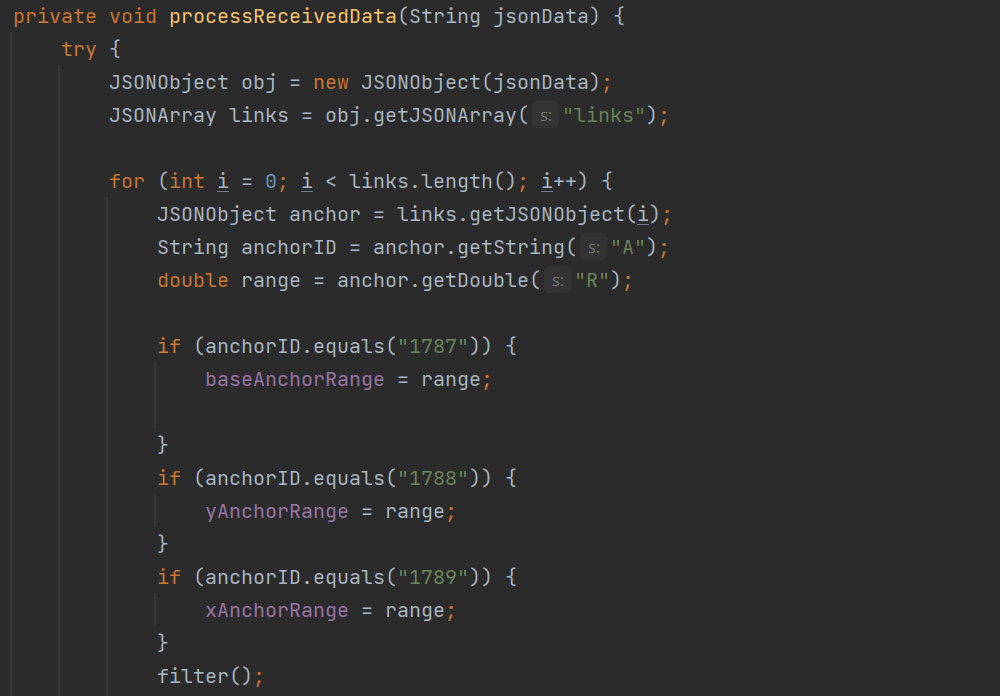
\includegraphics[width=0.5\linewidth]{images/EintragungVariablen.png}
	\caption[EintragungVariablen]{Eintragung in die Variablen}
	\label{fig:Variableneintragung}
\end{figure}

\begin{figure}[H]
	\centering
	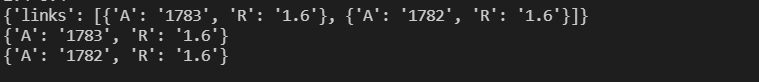
\includegraphics[width=0.5\linewidth]{images/JSONData.png}
	\caption[JSONData]{JSON Datenstruktur}
	\label{fig:JSONData}
\end{figure}

\begin{lstlisting}[style=Java, caption=Trilateration in Java, captionpos=b]
	private double[] trilaterate(double d1, double d2, double d3) {
		double x1 = ANCHORS[0][0], y1 = ANCHORS[0][1];
		double x2 = ANCHORS[1][0], y2 = ANCHORS[1][1];
		double x3 = ANCHORS[2][0], y3 = ANCHORS[2][1];
		
		double A = 2 * (x2 - x1);
		double B = 2 * (y2 - y1);
		double C = d1 * d1 - d2 * d2 - x1 * x1 - y1 * y1 + x2 * x2 + y2 * y2;
		
		double D = 2 * (x3 - x1);
		double E = 2 * (y3 - y1);
		double F = d1 * d1 - d3 * d3 - x1 * x1 - y1 * y1 + x3 * x3 + y3 * y3;
		
		double denominator = (A * E - B * D);
		if (denominator == 0) {
			System.out.println("ERROR: Denominator is zero, positions may be collinear!");
			return new double[]{-1, -1};
		}
		
		double x = (C * E - F * B) / denominator;
		double y = (C * D - A * F) / denominator;
		System.out.println("Calculated Tag Position: (" + x + ", " + y + ")");
		return new double[]{x, y};
	}
\end{lstlisting}
\section{GUI}
In diesem Abschnitt wird das GUI thematisiert.

\subsection{GUI-Setup}
Um das Programm zu verwenden, muss sich der Benutzer zunächst einloggen \ref{fig:StageControlViewGUI}. Die Benutzerkonten werden zuvor von einem Administrator in der Datenbank \ref{tab:users} \texttt{users} angelegt.  

Nach dem Login gelangt man zu einer Übersicht, in der ein oder zwei Geräte (Tags) hinzugefügt werden können. Anschließend müssen die Anchors festgelegt werden. Dazu bewegt man den Tag auf der Bühne zu einer Ecke und betätigt den Knopf „xy“. Danach wiederholt man diesen Schritt für eine weitere Ecke (oben in der Mitte), indem man erneut den Knopf „xy“ drückt. Sobald alle Anchors gesetzt sind, wird der MaxX-Wert zwischen Anchor1 und Anchor2 bestimmt, um den Servo zu steuern. Dies geschieht durch einen Klick auf den Knopf „xy“.  

Nach diesen Schritten sind sowohl die Visualisierung als auch die Servosteuerung funktionsfähig.

%% Bilder!!!

\subsection{GUI-Entwicklung}
Für die GUI-Entwicklung verwenden wir IntelliJ IDEA mit JavaFX, da uns das bereits vom Unterricht bekannt ist und wir somit nicht die Grundlagen einer anderen IDE lernen mussten.

Die GUI wird in verschiedene Szenen aufgeteilt, in unserem Fall in \textit{anlagen-view.fxml}, \textit{splash-view.fxml} \& \textit{stagecontrol-view.fxml}
Anbei ein Auszug aus der \textit{stagecontrol-view}:

\begin{figure}[H]
	\centering
	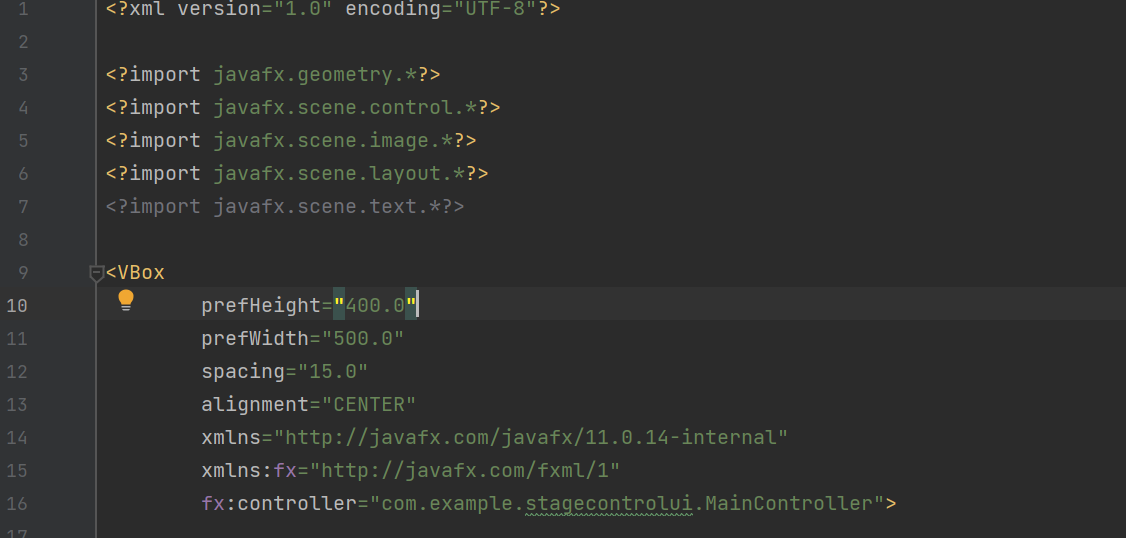
\includegraphics[width=0.5\linewidth]{images/stagecontrol-view.png}
	\caption[Auszug aus Stagecontrol-View.fxml]{Auszug aus Stagecontrol-View.fxml}
	\label{fig:Stagecontrolview}
\end{figure}

Dieser Code stell diese Szene dar:
\begin{figure}[H]
	\centering
	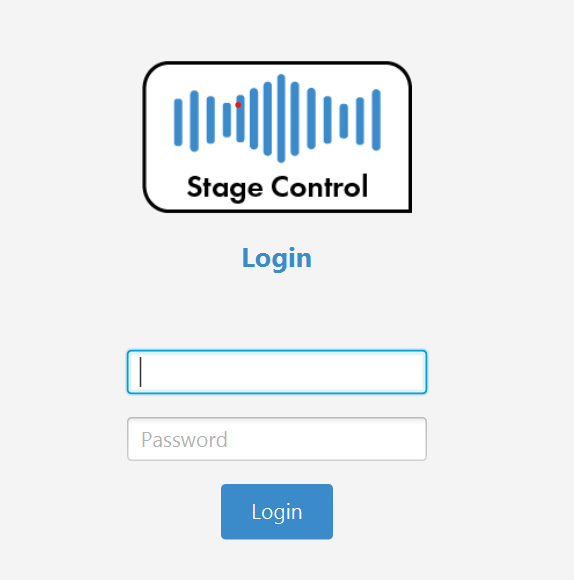
\includegraphics[width=0.5\linewidth]{images/StagecontrolViewGUI.png}
	\caption[StageControl GUI View]{StageControl GUI View}
	\label{fig:StageControlViewGUI}
\end{figure}


Jede Klasse bekommt einen Controller. Zum Beispiel: \textit{Main.java} hat einen Controller \textit{MainController.java}. Das hilft dabei einen guten Überblick über das Programm und seine Funktionalitäten zu behalten. Die Methoden werden in Java-Klassen umgesetzt und dann in einem FXML file aufgerufen, um zu funktionieren.

\subsection{GUI-Design}
Um alle Szenen korrekt zu laden haben wir eine Logo-Animation eingefügt. Damit schaffen wir außerdem einen Wiedererkennungswert, welcher uns sehr wichtig ist. Weiters um ein einheitliches Design zu gewährleisten, wurde jede Szene in der Mitte oben mit dem StageControl Logo versehen. Es wurden alle Farben aus der Cooperate Identity verwendet. Die User-Expierence wurde vereinfacht und für den Enduser optimiert.   

%% Bild von fertiger GUI

\section{Transferprotokolle}
In diesem Abschnitt werden die Transferprotokolle thematisiert.

\subsection{UDP}
UDP (=User Datagram Protocol) ist ein Kommunikationsprotokoll, welches Verbindung mit geringer Verlusttolerenz zwischen dem Internet und einer Anwendung herstellt. UDP ermöglicht die Prozess-zu-Prozess Kommunikation. Wir verwenden es, um die Daten vom ESP32 UWB an den RaspberryPi mit der Servosteuerung zu senden, und dort den Servowinkel zu berechnen. Hierfür verwenden wir eine statische IP bei sowohl RaspberryPi als auch bei dem ESP32 UWB selbst. Über den Port 80 sendet der ESP32 UWB, dann das Paket in einem JSON Format zum GUI. Dieser verarbeitet dies in einer Funktion und berechnet sich aus den Daten die Position des Tags. Wiederrum sendet das GUI wieder über UDP dem RaspberryPi die Position für die Winkelberechnung. \parencite{UDP}

\subsection{MQTT}
MQTT (=Message Queuing Telemetry Transport) ist ein offenes Protokoll für Verbindungen in unzuverlässige Netzwerke oder eingeschränkten Bandbreitenressourcen. \parencite{MQTT}

\subsection{MQTT vs UDP}
In der unteren Tabelle sieht man die Unterschiede zwischen MQTT und UDP.
\begin{table}[H]
	\centering
	\begin{tabular}{|l|c|c|}
		\hline
		\textbf{Merkmal} & \textbf{UDP} & \textbf{MQTT} \\
		\hline
		Verbindungstyp & Verbindungslos & Verbindung \\
		\hline
		Zuverlässigkeit & Niedrig & Wählbar (QoS) \\
		\hline
		Sicherheit & Keine Garantie & Wählbar (QoS) \\
		\hline
		Verzögerung & Gering & Gering (leichtgewichtig) \\
		\hline
		Anwendung & Streaming, Online-Spiele & IoT, Benachrichtigungen \\
		\hline
		Modus & Peer-to-Peer & Publish/Subscribe \\
		\hline
	\end{tabular}
	\caption{Vergleich von UDP und MQTT}
	\label{tab:udp_mqtt}
	\textcite{MQTTvsUDP}
\end{table}

\section{Datenbank}
Als Datenbank nutzen wir PostgreSQL. Diese Software ist Open-Source \parencite{PostgreSQL}, ein wichtiger Aspekt für unsere Diplomarbeit. 

\begin{figure}[H]
	\centering
	
\includegraphics[width=0.5\linewidth]{images/postgres-logo.png}
	\caption[PostgreSQL Logo]{PostgreSQL Logo}
	\label{fig:PostgreSQLLogo}
\end{figure}

\subsection{VMware Workstation Pro}
Die Software \texttt{VMware Workstation Pro} wurde verwendet, um eine virtuelle Maschine mit Ubuntu Server zu erstellen, auf der unsere PostgreSQL-Datenbank läuft. Da wir weder Ressourcen noch den Zugang zu einem physischen Server haben, haben wir uns für eine digitale Lösung entschieden. Außerdem ist es einfacher, eine digitale Datenbank einzurichten, als jedes Mal einen neuen physischen Server bereitzustellen.

\subsection{Datenbankstruktur}
\begin{table}[h]
	\centering
	\begin{tabular}{|l|l|}
		\hline
		\textbf{Column} & \textbf{Type} \\
		\hline
		id & integer \\
		\hline
		device\_id & integer \\
		\hline
		maxdistance & double precision \\
		\hline
		timestamp & timestamp without time zone \\
		\hline
	\end{tabular}
	\caption{Übersicht der Spalten und Datentypen der Tabelle \texttt{stagedata}.}
	\label{tab:stagedata}
\end{table}

Die Tabelle \texttt{stagedata} speichert Sensordaten, wobei jede Zeile eine eindeutige ID erhält. Die Spalten enthalten die Geräte-ID (Tag 1 oder Tag 2) (\texttt{device\_id}), die maximale Distanz zwischen Anchor1 und Anchor2 auf der x-Achse (\texttt{maxdistance}) und einen Zeitstempel (\texttt{timestamp}), der automatisch den aktuellen Zeitpunkt speichert, um Daten nachvollziehen zu können.


\begin{table}[h]
	\centering
	\begin{tabular}{|l|l|}
		\hline
		\textbf{Column} & \textbf{Type} \\
		\hline
		device\_id & integer \\
		\hline
		device\_name & character varying(255) \\
		\hline
		device\_type & character varying(100) \\
		\hline
		created\_at & timestamp without time zone \\
		\hline
	\end{tabular}
	\caption{Übersicht der Spalten und Datentypen der Tabelle \texttt{devices}.}
	\label{tab:devices}
\end{table}

Die Tabelle \texttt{devices} speichert Informationen über Geräte. Jedes Gerät (Tag) erhält eine eindeutige \texttt{device\_id}. Zusätzlich gibt es einen Gerätenamen (\texttt{device\_name}) und einen Gerätetyp (\texttt{device\_type}). Der Zeitstempel \texttt{created\_at} wird automatisch mit dem aktuellen Zeitpunkt gesetzt.

\begin{table}[h]
	\centering
	\begin{tabular}{|l|l|}
		\hline
		\textbf{Column} & \textbf{Type} \\
		\hline
		id & integer \\
		\hline
		username & character varying(50) \\
		\hline
		password & character varying(255) \\
		\hline
	\end{tabular}
	\caption{Übersicht der Spalten und Datentypen der Tabelle \texttt{users}.}
	\label{tab:users}
\end{table}

Die Tabelle \texttt{users} speichert Benutzerinformationen. Jedes Benutzerkonto erhält eine eindeutige \texttt{id}. Der \texttt{username} dient als Anmeldekennung und hat eine maximale Länge von 50 Zeichen. Das Feld \texttt{password} speichert das Passwort in gehashter Version des Benutzers, um sich dann folglich in der GUI anmelden zu können.

\subsection{Beziehung zwischen \texttt{devices} und \texttt{stagedata}}

Die Tabellen \texttt{devices} und \texttt{stagedata} stehen in einer 1-zu-N-Beziehung. Jedes Gerät in der Tabelle \texttt{devices} kann mehrere zugehörige Sensordaten in der Tabelle \texttt{stagedata} besitzen. Dies wird durch die Spalte \texttt{device\_id} in \texttt{stagedata} realisiert, die als Fremdschlüssel auf \texttt{device\_id} in \texttt{devices} verweist. Dadurch wird ermöglicht, dass jede die Daten einem existierenden Gerät zugeordnet ist. 

\subsection{Nützliche Befehle für PostgreSQL}
\textbf{psql} \ – connects you to the psql shell. \\
\textbf{\textbackslash{c}} \ – connects to the database. \\
\textbf{\textbackslash{l}} \ – shows all databases. \\
\textbf{\textbackslash{d}} \ – shows all tables. \\
\textbf{\textbackslash{d} tablename} \ – shows table details. \\
\textbf{\textbackslash{q}} \ – quit the psql.

Diese Funktionen sind die Grundlagen und helfen dabei sich in einer Datenbank, wie PostgreSQL zu recht zu finden.

\section{Corporate Identity}
Bei der Corporate Identity beschäftigt sich Stage Control mit der Namensfindung, Farben, Logo, sowie der Schriftart. Nach der Namensfindung wurden die passenden Farben und das Logo geplant, sowie gestaltet.

\subsection{Namensfindung}
Ein sehr ausschlaggebender Teil einer Marke ist der Name, dieser sollte gut überlegt werden. Für die Namensfindung von Stage Control wurde ein Meeting mit dem Projektteam veranlasst, in welchem Namensvorschläge überlegt und präsentiert wurden. 
Anfänglich lag der Fokus auf den Worten Stage, Automation und Sound, da es hauptsächlich um die Steuerung von Audioanlagen auf einer Bühne geht. In diesem Zusammenhang sammelten wir Namensideen, die in der nachstehenden Abbildung \ref{fig:Brainstorming_Namensfindung} aufgelistet sind. 

\begin{figure}[H]
	\centering
	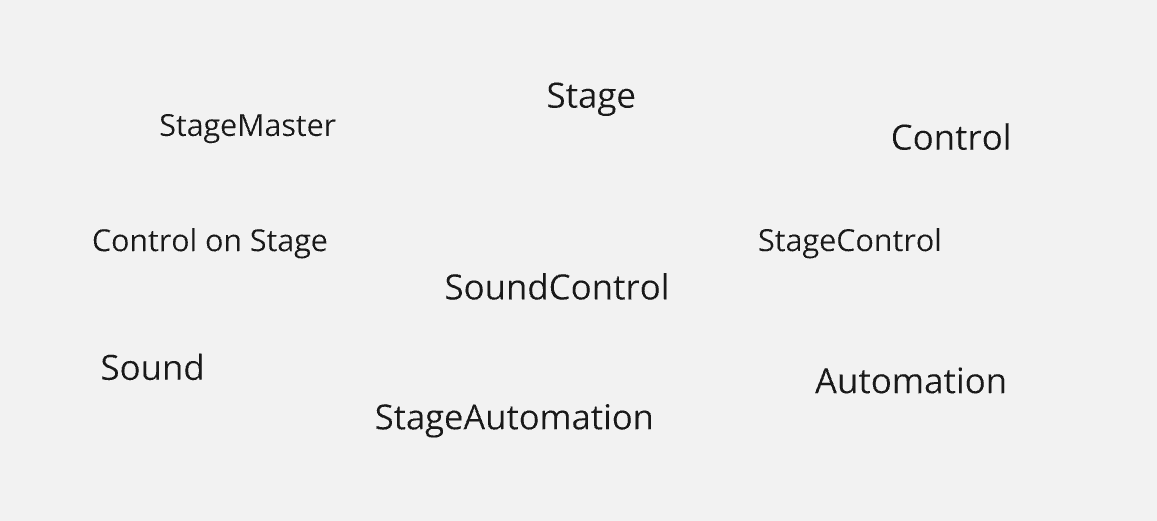
\includegraphics[width=0.5\linewidth]{images/Brainstorming_Namensfindung.png}
	\caption[Brainstorming Namensfindung]{Brainstorming Namensfindung}
	\label{fig:Brainstorming_Namensfindung}
\end{figure}

Schlussendlich einigte sich unser Projektteam auf den Namen Stage Control, da es genau beschreibt um welche Tätigkeit es sich bei dieser Arbeit handelt. ‘Stage Control‘ ist Englisch und bedeutet Bühnensteuerung. 

\subsection{Unternehmensfarben}
Stage Control entschied sich für bläuliche Töne als Unternehmensfarben. Die Farbe Blau steht für Treue, Sicherheit, Kreativität, Produktivität und Technik. \parencite{BedeutungderFarbeBlau} Diese Merkmale möchte Stage Control damit ausstrahlen. Die ausgewählte Farbpalette von Stage Control ist in der Abbildung \ref{fig:Hexcode} zu sehen. 

\begin{figure}[H]
	\centering
	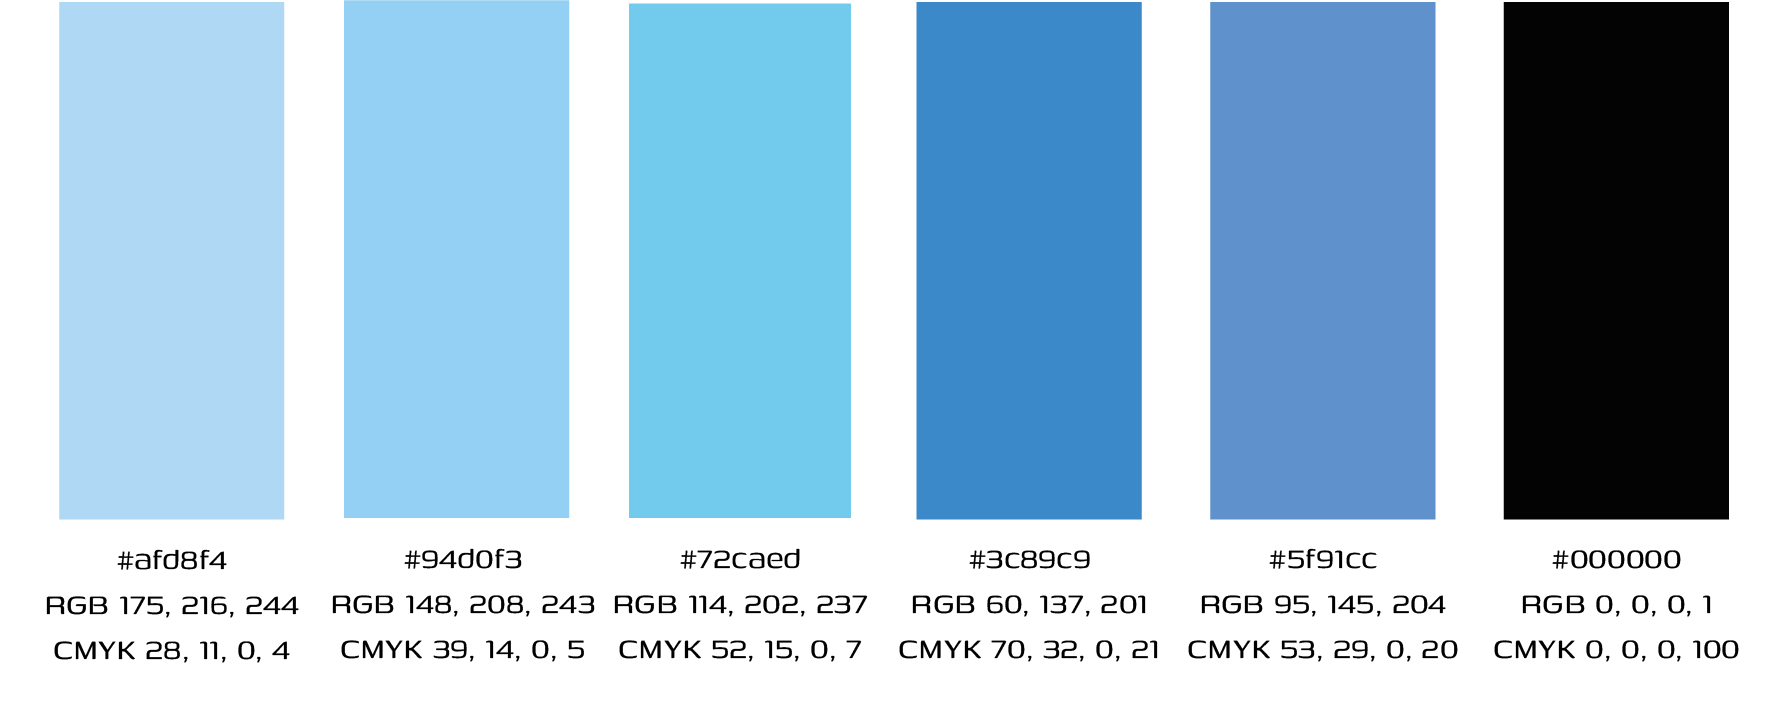
\includegraphics[width=0.7\linewidth]{images/Hexcode.png}
	\caption[Die Hex Codes von Stage Control]{Die Hex Codes von Stage Control}
	\label{fig:Hexcode}
\end{figure}


\subsection{Logo}
Nach der Festlegung des Projektteamnamens überlegte sich Stage Control Ideen, wie das Logo aussehen könnte. Aufgrund des ausgewählten Namens startete das Brainstorming mit einer Bühne im Logo. Der erste Entwurf ist in der nachstehenden Abbildung \ref{fig:Logoentwurf1} ersichtlich. 

\begin{figure}[H]
	\centering
	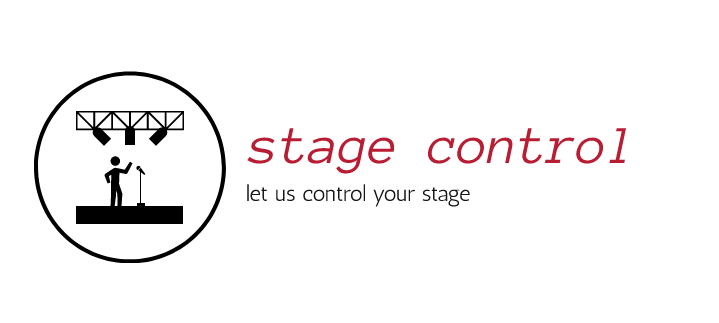
\includegraphics[width=0.5\linewidth]{images/Logoentwurf1.png}
	\caption[Erster Logoentwurf]{Erster Logoentwurf}
	\label{fig:Logoentwurf1}
\end{figure}

Doch dieser Ansatz vom Logo passte nicht. Es war nichts Einzigartiges und es war uneinprägsam. Weiters beinhaltete der erste Entwurf zu viel Text. 

Als zweiten Entwurf wurden Soundbalken dargestellt, sodass die ursprüngliche Idee auch im Logo zu sehen ist. Da im Namen nur die Bühnensteuerung vorkommt und nicht erkennbar ist um was es sich genau handelt. In Abbildung \ref{fig:Logoentwurf2} ist der Entwurf zu sehen. Jedoch passten die Soundbalken noch nicht. Der Entwurf wirkte schlicht und unauffällig, wodurch es nicht zu Stage Control passt. 

\begin{figure}[H]
	\centering
	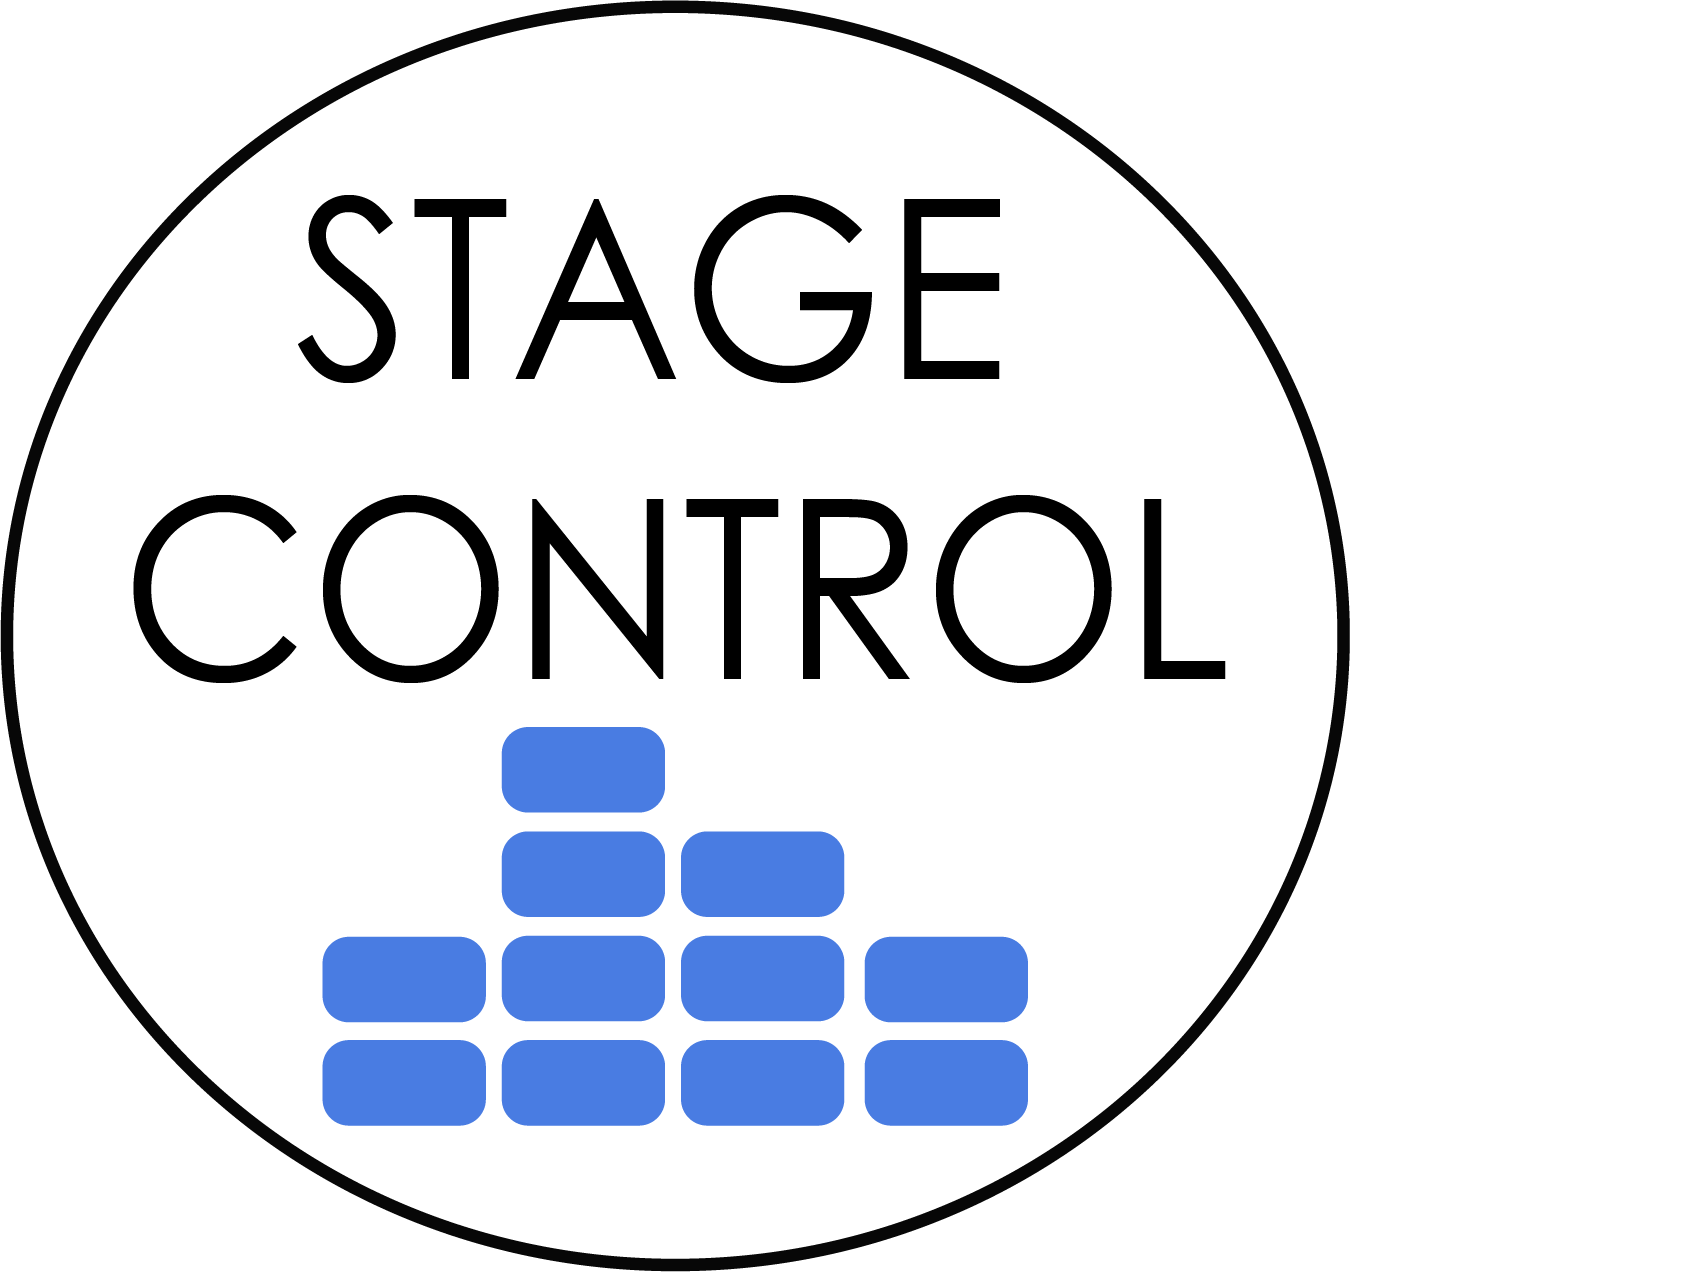
\includegraphics[width=0.5\linewidth]{images/Logoentwurf2.png}
	\caption[Zweiter Logoentwurf]{Zweiter Logoentwurf}
	\label{fig:Logoentwurf2}
\end{figure}

Der dritte und letzte Entwurf bestand ebenfalls als Soundbalken. Nur wurde hier eine anderen Anordnung, sowie eine andere Position des Textes gewählt. Weiters wurde bei diesem Logo der Rahmen ansprechender designt, sodass das Logo modern wirkt und einprägsamer ist. In Abbildung \ref{fig:Logo_StageControl} ist das endgültige Logo zu sehen.

\begin{figure}[H]
	\centering
	
\includegraphics[width=0.5\linewidth]{images/Logo_StageControl.png}
	\caption[Logo von Stage Control]{Logo von Stage Control}
	\label{fig:Logo_StageControl}
\end{figure}

\subsubsection{Erstellung des Logos}
Für die Erstellung des Logos wurde das Programm Adobe Illustrator verwendet. Adobe Illustrator ist praktisch, da im Nachhinein jederzeit die Formen verändert werden können. Bei den Formen kann man Ankerpunkt setzen, diese können hinzugefügt, verschoben oder gelöscht werden. Weiters kann man verschiedene Ebenen erstellen und diese jederzeit ein, sowie ausblenden. Zusätzlich haben wir in diesem Programm schon einige Erfahrungen im Laufe der Schulzeit gesammelt. 

Nach der Wahl des Programmes wurde der erste Prototyp des Logos entworfen. Den Beginn der Logofertigstellung bildeten die Soundbalken in unterschiedlichsten Größen, hierfür wurde für jeden Balken eine eigene Ebene erstellt. Die Soundbalken wurden als Rechtecke eingefügt und die Ecken abgerundet. Nach dem Erstellen von diesen Balken wurden diese blau eingefärbt. 

Danach wurde überlegt, ob der Projektname rechts, oben oder unten positioniert werden soll. Letztendlich wurde der Text unter den Soundbalken positioniert, da der Name hier am übersichtlichsten erscheint. Hierbei wurde auch jeder Buchstabe in einer eigenen Ebene angelegt. 

Als nächstes stand die Wahl der Schriftart des Logos an. Wir entschieden uns für die Schrift „Futura PT Demi“ da diese gut zu unserem Logo und unserer Arbeit passte. Ein Anliegen war uns, dass die Schrift nicht zu dünn ist, sodass diese gut leserlich ist und nicht im Logo untergeht. Als Schriftgrße entschieden wir uns für 27pt, da der Text sonst im Logo untergehen würde. 

Schlussendlich fehlte noch ein Rahmen für das Logo. Hierbei sollte es nichts Einfaches sein, da ein Kreis oder Rechteck wenig Aufmerksamkeit erregt. Daher überlegten wir uns die Ecken des Rechteckes auf drei Seiten abzurunden. Somit wirkt das Logo modern, als würde eine Nachricht aufpoppen. 

\section{Werbematerial}
Um Interessenten von Stage Control zu überzeugen, wurde als Werbematerial ein Flyer erstellt. Der für die Bekanntheit der Marke sorgt.

\subsection{Flyer}
Der Flyer ist eines der wichtigsten Werbemitteln im Marketing. Ein Flyer sollte handlich sein und eine perfekte Größe zum Lesen haben. Es ist unabhängig vom Internet und billiger als große Plakatwerbungen oder Anzeigen. Weiters ist ein Flyer informativer als eine Anzeige und es lässt die Leser mehr über das Unternehmen oder das Projekt erfahren. Ein Flyer ist außerdem nicht nur ein Fließtext, es beinhaltet auch Bilder und verschiedenstes Design, welches zum Weiterlesen anregt. Der Flyer sollte nicht zu viel Text beinhalten, da dies oft für Leser zu kompliziert oder uninteressant wirken könnte. Besser wäre es, wenn ein Flyer schlicht und mit einem ansprechendem Design gestaltet worden ist. \parencite{VorteilevonFlyern}

\subsubsection{Erstellung des Flyers}
Für die Erstellung des Flyers wurde das Programm Adobe InDesign verwendet. Schon am Anfang stand fest, dass der Flyer 4 Seiten haben wird. Der nächste Schritt war die Planung des Flyers, wo beschlossen wurde welche Informationen vorhanden sein sollten und wie die Positionierung erfolgen wird. Danach wurde ein neues Dokument in InDesign erstellt und die Grundeinstellungen wie Seitenformat, Anzahl der Seiten und Ränder festgelegt. Wir entschieden uns pro Seite für eine Höhe von 210mm und einer Breite von 100mm. Das Dokument wurde im Querformat eingerichtet und Spalten erstellt, die die Seiten des Flyers bilden. Um alle vier Seiten des Flyers bearbeiten zu können, verfügt das Dokument zwei Seiten. Hierbei wurden Hilfslinien eingeblendet, da diese die Arbeitsbereiche voneinander abgrenzen. Diese wurden danach gesperrt, sodass die Hilfslinien während des Arbeitens nicht unabsichtlich verschoben werden. 

Das Design und das Layout wurden sorgfältig ausgewählt, um ein einheitliches Erscheinungsbild darzustellen. Die Farben wurden von den Unternehmensfarben verwendet. Zudem wurde auch das Logo von Stage Control verwendet. Als Designelemente entschieden wir uns für Dreiecke, da diese gut zu unserem Design passten. 

Die Schriftart Genos wird für die Textinhalte des Flyers verwendet. Diese Schriftart bietet eine gut leserliche und moderne Schrift für den Text. Durch die Kombination von selbstgemachten Fotos, Formen, Farben und der modernen Schriftart wirkt der Flyer sehr ansprechend. 

\subsubsection{Inhalt des Flyers}
Die Titelseite des Flyers beinhaltet rechts oben das Logo von StageControl. Wie in der Abbildung \ref{fig:Titelseite} zu sehen ist, wurde ein Foto von einem Mischpult fotografiert. Welches mit Dreiecken ansprechend umschlossen wird, dies hat nicht nur eine ästethische Wirkung, sondern weckt auch das Interesse der Leser, da man auf dem ersten Augenblick erkennen kann um was es sich hierbei handelt. 
Die Schriftgröße des Namens wurde mit 34pt verwendet, da es eines der wesentlichsten Details von der Titelseite ist. Der Name wurde von der Kurzbeschreibung, welche mit 19pt geschrieben wird, mittels einer Linie getrennt. Somit ist die Kurzbeschreibung abgetrennt von der Überschrift, dadurch wirkt die Titelseite ansprechender.

\begin{figure}[H]
	\centering
	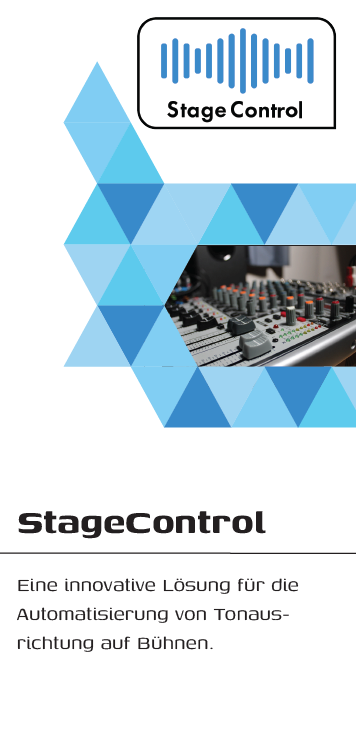
\includegraphics[width=0.5\linewidth]{images/Titelseite.png}
	\caption[Titelseite]{Titelseite}
	\label{fig:Titelseite}
\end{figure}

Auf den nächsten beiden Seiten befindet sich die Informationsseite. Auf der linken Innenseite wird erklärt, was StageControl macht und wieso es wichtig ist, dass diese Arbeitsweise automatisiert wird. Auf der rechten Innenseite wird erklärt wie StageControl funktioniert. Es dient als Anleitung, sodass der Leser eine kurze Beschreibung hat. Somit ist ersichtlich, wie die Steuerung von Tonanlagen mit StageControl umgesetzt werden. Um in diesen Innenseiten des Flyers auch etwas Farbe zu bekommen, wurden hier dieselben Dreiecke wie auf der Titelseite verwendet. Somit wirkt es nicht kalt, da der Text mithilfe von den Dreiecken umschlossen wird. Um die Innenseiten ansprechender zu gestalten, überlegte sich StageControl einen Verlauf der Dreiecke von der rechten Seite auf die linke Seite. Wie in der Abbildung \ref{fig:Informationsseite} zu sehen ist.

\begin{figure}[H]
	\centering
	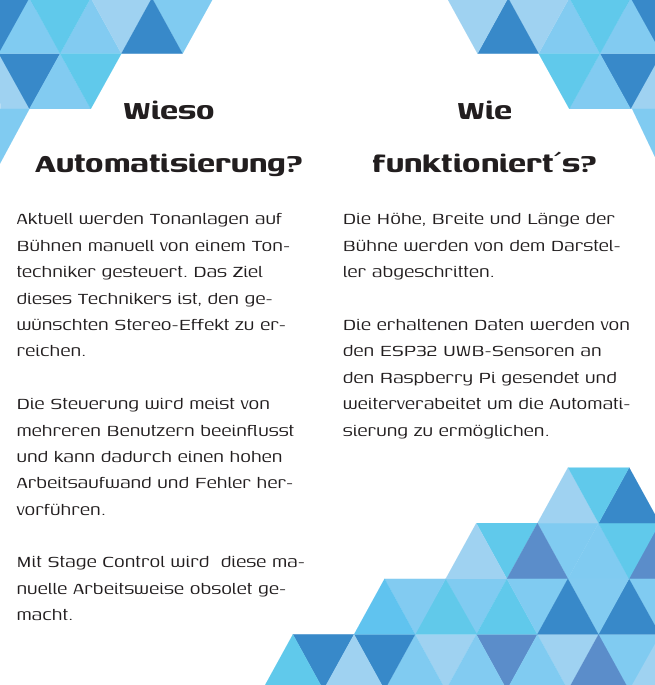
\includegraphics[width=0.5\linewidth]{images/Informationsseite.png}
	\caption[Informationsseite]{Informationsseite}
	\label{fig:Informationsseite}
\end{figure} 

Auf der letzten Seite stellt sich das Team von StageControl vor, welches in der Abbildung \ref{fig:Teamseite} ersichtlich ist. Ein Gesamtbild des Projektteams ist wichtig um das Vertrauen des Lesers zu gewinnen. Außerdem bekommt der Leser einen ersten Einblick vom Team und kann hiermit schon feststellen, ob ihm das Team, sowie das Konzept zusagt. Weiters wird das Team von StageControl beschrieben und erklärt wie wir es geschafft haben, uns dieser Herausforderung zu stellen.

\begin{figure}[H]
	\centering
	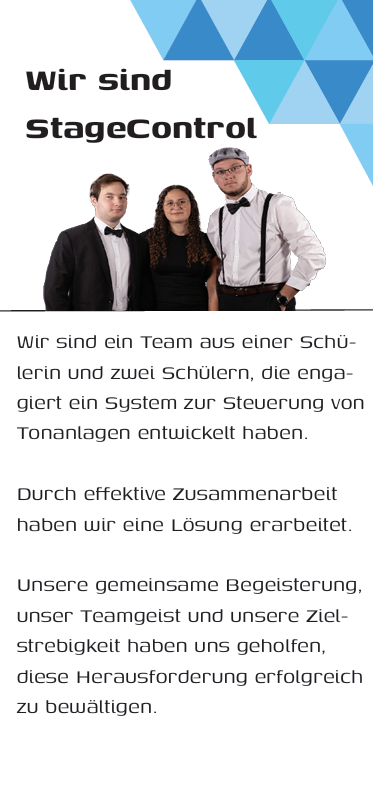
\includegraphics[width=0.5\linewidth]{images/Teamseite.png}
	\caption[Teamseite]{Teamseite}
	\label{fig:Teamseite}
\end{figure} 

Die einzelnen Themen im Flyer sind wichtig, um somit dem Leser einen umfassenden Einblick in StageControl zu geben und sie zu begeistern StageControl zu verwenden. Durch der Kombination von Informationen und des Designs wurde ein informativer Flyer entwickelt. 

\section{Logo Animation}
Für die Erstellung einer Animation vom Logo wurde das Programm Adobe After Effects verwendet. Als erstes wurde die Illustratordatei von dem Logo importiert, indem eine neue Komposition erstellt wurde. Wobei hier darauf geachtet werden muss, dass die Ebenengrößen beibehalten werden. Die Kompositionsdateien werden links im Projekt-Panel angezeigt, wie in der nächsten Abbildung \ref{fig:Projekt-Panel} zu sehen ist.

\begin{figure}[H]
	\centering
	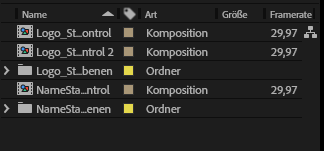
\includegraphics[width=0.5\linewidth]{images/Projekt-Panel.png}
	\caption[Projekt-Panel]{Projekt-Panel}
	\label{fig:Projekt-Panel}
\end{figure} 

Mit einem Doppelklick auf die Animationskomposition, wird die Datei geöffnet und in der Zeitleiste, die sich unten befindet, werden alle Ebenen angezeigt. 

\begin{figure}[H]
	\centering
	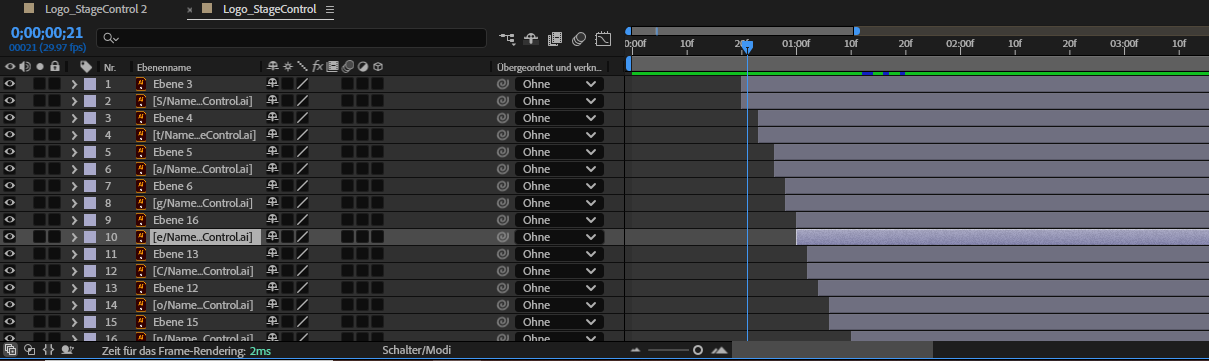
\includegraphics[width=0.5\linewidth]{images/Zeitleiste.png}
	\caption[Zeitleiste]{Zeitleiste}
	\label{fig:Zeitleiste}
\end{figure} 

Da jeder Balken und Buchstabe eine eigene Ebene war, konnte in der Zeitleiste einfach die jeweilige Ebene an die gewünschte Position hingeschoben werden. Somit konnte die Annordnung der Balken und Buchstaben in Sekundenabständen mittels einem Verlauf dargestellt werden. Mithilfe des Vorschau-Panels konnte das Ergebnis der Animation direkt angeschaut werden. 

\begin{figure}[H]
	\centering
	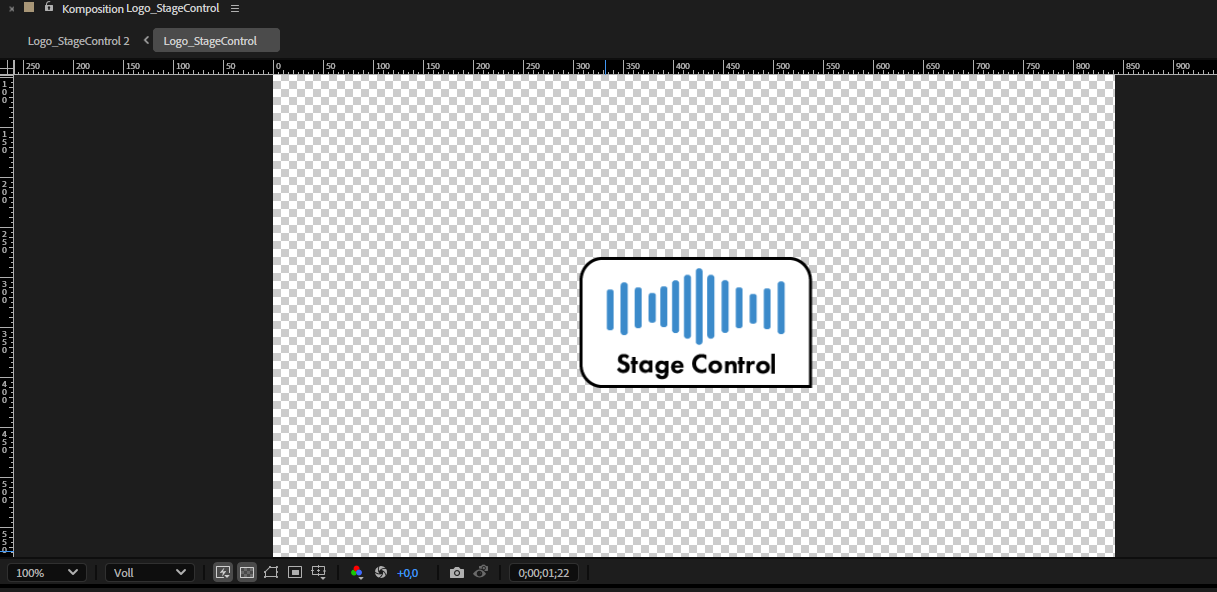
\includegraphics[width=0.5\linewidth]{images/Vorschau-Panel.png}
	\caption[Vorschau-Panel]{Vorschau-Panel}
	\label{fig:Vorschau-Panel}
\end{figure} 

\section{SD-Kartensicherung}
Für das Klonen von einer SD-Karte wird eine zusätzliche SD-Karte, sowie ein SD-Kartenleser benötigt. Als erstes wählten wir das Programm Win32 Disk Imager aus und installierten es. Den Prozess des SD-Karten klonen machten wir mit folgender Anleitung. \parencite{SD-Kartenklonen}
Danach wurde die zu klonende SD-Karte in den Kartenleser des PCs gesteckt. Als nächstes wurde Win32 Disk Imager gestartet und rechts oben im Programm in der Dropdown-Liste „Device“ das Laufwerk des Kartenlesers ausgewählt. Dann wurde auf das Ordner Symbol links daneben geklickt und der Speicherort eingegeben. Als nächstes wurde auf den Button „Read“ geklickt, um den Vorgang zu starten. Nach dem Prozess wurde die SD-Karte entfernt und die leere SD-Karte in das Lesegerät gesteckt. Es wurde sichergestellt, dass die zuvor erstellte Image-Datei ausgewählt ist, falls dies nicht der Fall wäre, sollte es durch das Ordner Symbol wieder eingestellt werden. Danach wurde wieder der Kartenleser in „Device“ ausgewählt und abschließend auf den Button „Write“ geklickt. Nun wurde auf der zweiten SD-Karte eine exakte Kopie von der ersten SD-Karte erstellt. In der nachstehenden Abbildung \ref{fig:Win32 Disk Imager} ist der Prozess der SD-Karten Sicherung zu erkennen.

\begin{figure}[H]
	\centering
	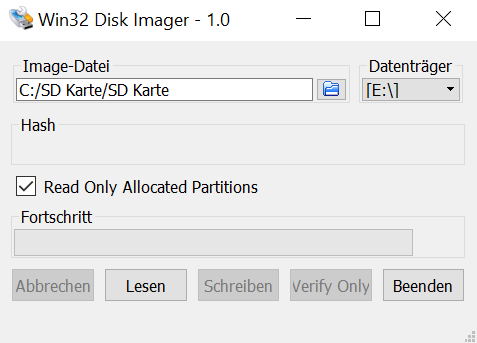
\includegraphics[width=0.5\linewidth]{images/Win32 Disk Imager.png}
	\caption[Win32 Disk Imager]{Win32 Disk Imager}
	\label{fig:Win32 Disk Imager}
\end{figure}

\section{Raspberry Pi als Access Point}
Der Einsatz des Raspberry Pis als Access Point dient, dazu die Services wie Dnsmasq und Hostapd zu nutzen um ein lokales Wlan-Netzwerk aufzubauen. Da der Raspberry Pi ein WLAN-Modul besitzt, wurde dieser als AccessPoint eingerichtet, somit kann das Netzwerk überall aufgebaut werden.  
Für das konfigurieren des Raspberry Pis als Access Point wurde die Anleitung von AZ-Delivery \textit{"Raspberry Pi als AccessPoint"} zur Hilfe genommen. Als erstes wurde die Wlan-Netzwerkschnittstelle mit einer festen IP konfiguriert. Diese Konfiguration ist wichtig, da der Raspberry Pi nun eine feste IP-Adresse auf der WLAN-Schnittstelle bekommt. Eine WLAN(Wireless Local Area Network)-Schnittstelle ist eine drahtlose Netzwerkschnittstelle, die es ermöglicht eine Verbindung mit dem WLAN herzustellen. Als nächstes wurde der DHCP-Client auf der WLAN-Schnittstelle deaktiviert.  Danach wurde der Raspberry PI neugestartet und ein DHCP-, sowie DNS-Server installiert und konfiguriert. Ein DHCP Server, auch Dynamic Host Configuration Protocol Server genannt, stellt einem Internetprotokollhost automatisch seine IP-Adresse zuweist. Ein DNS-Server hingegen funktioniert, wie ein Telefonbuch, es verwaltet die Domain und deren zugehörige IP-Adressen. Der DNS-Server übersetzt die Domainanforderungen in IP-Adressen und steuert dabei, welchen Server ein Endnutzer erreicht, wenn er in seinem Browser einen Domain Namen eingibt.  Zum Schluss wurde noch ein Access Point installiert. Der AccessPoint wurde konfiguriert mit dem Namen "raspberry-wlan" und dem Passwort "stagecontrol". Nun kann mit dem WLAN eine Verbindung hergestellt werden. \parencite{RaspberryPiAccessPoint}

\begin{figure}[H]
	\centering
	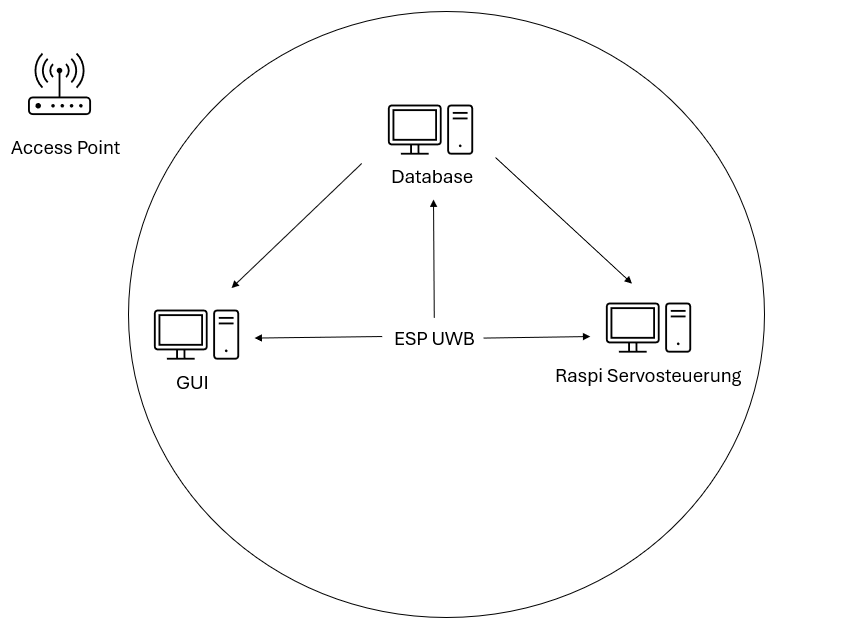
\includegraphics[width=0.5\linewidth]{images/Peer to Peer Netzwerk.png}
	\caption[Peer to Peer Netzwerk]{Peer to Peer Netzwerk}
	\label{fig:Peer to Peer Netzwerk} 
\end{figure}

Damit das Wlan gestartet wird wurde folgende Commandozeile eingegeben: 
\begin{lstlisting}
	sudo ip addr add 192.168.10.10/24 dev wlan0 
\end{lstlisting}

Im File /etc/dhcpcd.conf wurden folgende Commandozeilen eingegeben: 
\begin{lstlisting}
	interface wlan0
	static ip_addr=192.168.10.1/24
	static routers=192.168.10.1
	static doamin_name_servers=8.8.8.8.8.8.4.4
	nohook wpa_supplicant
\end{lstlisting}

Im File /etc/dnsmasq.conf wurde die Schnittstelle vom Internet eingerichtet:
\begin{lstlisting}
	interface=wlan0
	dhcp-range=192.168.10.100,192.168.10.200,24h
	
	dhcp-host=C8:2E:18:AD:7F:14,192.168.10.10
	dhcp-host=C8:2E:18:AD:7E:30,192.168.10.20
\end{lstlisting} 

Die oben genannten MAC Adresse \textit{Media Access Code Adresse} ist eine Nummer von einem Endgerät, die spezifisch für ein Gerät ist. Anhand von dieser Nummer werden über die Verbindung laufende Daten den Geräten zugeordnet. Nach jeder Veränderung wurde der Raspberry Pi neugestartet. 


\section{Gerüstbau}
StageControl benötigt ein Gerüst, in dass ein Mischpult hineingestellt wird, um eine sichere Ausführung der automatisierten Tonausrichtung zu gewährleisten. 


\begin{figure}[H]
	\centering
	\includegraphics[width=0.483\linewidth]{images/Gerüst-7.jpg}
		\includegraphics[width=0.4\linewidth]{images/Gerüst-8.jpg}
	\caption[Gerüstbau]{Gerüstbau}
	\label{fig:Gerüstbau}
\end{figure}


\subsection{Grundsätzliche Funktionalität}
Um dies sicherzustellen, wurde ein Gerüst aus Aluminiumstangen und Holzplatten gefertigt. Es ermöglicht, unterschiedlich große Mischpulte in das Gerüst zu stellen, ohne jegliche Anpassungen vornehmen zu müssen. Oberhalb wurde eine verschiebbare Stange befestigt, auf der ein Servomotor montiert werden kann.\\
An der Seite des Gerüsts befindet sich ein Platz für den Raspberry Pi und einen ESP32 UWB zur Befestigung mittels Schrauben.

\begin{figure}[H]
	\centering
	\includegraphics[width=0.4\linewidth]{images/Gerüst-2.jpg}
	\caption[Gerüst]{Gerüst}
	\label{fig:Gerüst-1}
\end{figure}



\subsection{Verwendete Materialien}
Für den Bau des Gerüsts wurden 4 x 1 m große Aluminiumstangen mit den Maßen 10 × 10 × 1000 mm verwendet, um den Rahmen zu konstruieren. Die Stangen wurden mit Schrauben und Muttern befestigt.\\

\begin{table} [H]
	\begin{tabular}{ |p{3.3cm} |p{4.8cm}|p{4.8cm}| }
		\hline
		\textbf{Material} & \textbf{Menge}& \textbf{Maße pro Stück}\\
		\hline
		\textbf{Aluminium Stangen} & 4x1m Aluminium Stangen & 10x10x1000mm  \\ 
		\hline
		\textbf{Holz-Grundplatte} & 2 Stück & 32x28cm   \\  
		\hline
		\textbf{Holz-Platte klein} & 1 Stück & 12x9.5cm   \\  
		\hline
		\textbf{Aluminium Flachprofil} & 2 Stück  & 1m \\
		\hline
		\textbf{Steckkappen Plastik} & 8 Stück & 10x10mm eckig  \\
		\hline
		\textbf{Befestigungswinkel}& 12 Stück für das Gerüst, 4 Stück zum Befestigen der Holzplatten   &  \\
		\hline
		\textbf{Schrauben}& 44 Schrauben für das gesamte Gerüst | 	Raspberry/ESP32 UWB Aufsatz & 42 Stück M4x20 | 2 Stück M4x40\\
		\hline
		\textbf{Muttern / Flügelmuttern}& 42 Muttern + 2 Flügelmuttern & \\
		\hline	
	\end{tabular}
	\caption{Stückliste Verwendete Materialien} 
\end{table} 




Um die Servomotoren an unterschiedliche Mischpulte anzupassen, wurden die Servomotoren auf einer verstellbaren Aluminium Flachstange montiert, auf der diese verschoben werden können. Zusätzlich kann man die Servomotoren auch horizontal justieren, indem die Mutter, die die Servomotoren hält, löst. \\
Um einen besseren Halt für die Mischpulte zu gewährleisten wurden zwei Holzplatten als Boden eingesetzt.

\begin{figure}[H]
	\centering
	\includegraphics[width=0.3\linewidth]{images/Gerüst-3.jpg}
	\caption[Gerüst]{Gerüst}
	\label{fig:Gerüst-2}
\end{figure}


\section{Servomotoren}
Die Servomotoren sind das Stück Hardware, ohne dass die automatische Tonausrichtung nicht funktionieren kann, deshalb ist es wichtig einen passenden Motor auszuwählen der unseren Kriterien entspricht. Diese Servomotoren müssen sehr robust sein damit er etwaige mechanische Einwirkung aushält. Außerdem müssen die Motoren wasserfest sein um auch bei außen Einsätzen nutzbar zu sein. 

\subsection{Servomotoren Auswahl}

Im Rahmen dieser Diplomarbeit wurde zur Steuerung der Drehpotentiometer die Savöx SH-0255MG Servo verwendet. Dieser wird über ein Python-Skript mit den entsprechenden Winkeldaten angesteuert. Die genaue Berechnungsmethode wird im Kapitel \ref{Steuerlogik} detailliert erläutert.

\section{Servomotoren Anpassungen}
Die Servomotoren werden in einem eigens Angefertigten Gestell gelegt und dann mittels 2 M4x20 Schrauben niedergeschraubt. Durch dieses Gestell werden die Servomotoren vor etwaigen mechanischen Einflüssen geschützt. \\
Dieses Gestell wird dann mit dem Servomotor zwischen dem Flachprofil und einer 10x10x1000mm Aluminiumstange mittels zwei Flügelmuttern niedergeschraubt.\\
Außerdem musste bei den Servomotoren ein Teil des Originalen Gehäuses abgeschliffen werden, um genug Platz für die Feststellschrauben zu haben.

\begin{figure}[H]
	\centering
	\includegraphics[width=0.4\linewidth]{images/Servo-Anpassungen.jpg}
	\caption[Servomotoren Anpassungen]{Servomotoren Anpassungen}
	\label{fig:Servomotoren Anpassungen}
\end{figure}


\section{Servomotor-Aufsatz}
Um den zuverlässigen Betrieb des Servomotors zu gewährleisten, wurde ein Aufsatz für den Servomotor im 3D-Druckverfahren hergestellt. Der Aufsatz besteht aus einem 4cm Zylinder mit einer vertikalen Öffnung für die  Abtriebswelle (Spline Shaft)  und einem rechteckigen Oberteil das aus dem Zylinder im 45 Grad herausragt, auf das der originalen Aufsatz des Servomotors geschraubt werden kann. Der Zylinder wird so auf dem Drehpotentiometer platziert, dass die Aussparung des Potentiometers mit der Öffnung des Aufsatzes übereinstimmt. Dadurch wird ein Übersteuern des Servomotors verhindert.

\begin{figure}[H]
	\centering
	\includegraphics[width=0.25\linewidth]{images/Servomotor+Aufsatz.jpg}
	\includegraphics[width=0.324\linewidth]{images/Aufsatz-Servo.jpg}
	\caption[Servomotor + Aufsatz]{Servomotor + Aufsatz}
	\label{fig:Servomotor + Aufsatz}
\end{figure}



\subsection{Entwicklungsprozess}
Um den idealen Aufsatz für die Drehpotentiometersteuerung zu entwickeln, waren einige Verbesserungen an der ersten Version erforderlich. Zunächst plante ich, den Aufsatz als Zylinder mit einer Höhe von 4 cm zu konstruieren und darauf einen kleineren Zylinder zu platzieren, der in die Spline Shaft gesteckt werden sollte. \\
Beim Testen zeigten sich jedoch sofort einige Probleme: Da es keine feste Verbindung zwischen der Spline Shaft und dem Aufsatz gab, drehte dieser über dem Drehpotentiometer durch. Zudem fehlte eine Ausbuchtung für den hervorstehenden Teil des Drehpotentiometers, die für die manuelle Ausrichtung von Vorteil ist.\\
Diese Verbesserungen wurden umgesetzt, und der fertige 3D-gedruckte Aufsatz verfügt nun über die in der Einleitung genannten Eigenschaften.


\begin{figure}[H]
	\centering
	\includegraphics[width=0.189\linewidth]{images/ReglerV1.png}
	\includegraphics[width=0.3\linewidth]{images/Regler.png}
	\caption[Regler-Aufsätze Versionen]{Regler-Aufsätze Versionen}
	\label{fig:Regler-Aufsätze Versionen}
\end{figure}

\subsection{Steuerlogik} \label{Steuerlogik}
Die Servomotoren werden dann immer bewegt wenn sich der Künstler auf der Bühne bewegt. Das bedeutet immer wenn der ESP32 UWB-Tag eine Veränderung der Position des Interpreten anhand der Anchor Positionen misst wird diese Position an den Raspberry Pi mittels MQTT-Protokoll geschickt und mit einem Python Programm in Winkel Grad umgewandelt. Anhand dieser Winkel kann sich nun der Servomotor bewegen. Wobei immer bedacht werden muss vor dem Verarbeiten der Position das nur die X-Achse der Bühne betrachtet wird und so Position X=0 = 0° und maxX=180° sind. Anhand dieser Extremwerte kann dann die Position in Winkel Grad umgewandelt werden.
\\Zur Veranschaulichung der Berechnung:\\\\
Der Künstler befindet sich auf der Bühne bei der Position X=5m, die Extrempunkte der Bühne sind X1=0m und X2=10m.\\
Der Raspberry Pi bekommt die Position des Künstlers mittels UDP übermittelt und rechnet diese anhand des Extremwerts X2 in Winkel Grad um. Das bedeutet bei X2=10m und Position des Interpreten bei 5m, dass sich der Servo, der für genau den einen Künstler zuständig ist, auf 90° stellen muss. \\

\begin{lstlisting}
	def move_servo(value):
	global max_x
	
	try:
	if max_x is None or max_x == 0:
	print(f"Invalid max_x value: {max_x}. Servo will not move.")
	return
	
	angle = (value / max_x) * 180
	angle = max(0, min(180, angle)) 
	
	duty = 2 + (angle / 18)
	print(f"Moving servo to {angle} (Duty Cycle: {duty})")
	
	pwm.ChangeDutyCycle(duty)
	sleep(0.3)
	pwm.ChangeDutyCycle(0) 
	
	except Exception as e:
	print(f"Error moving servo: {e}")
\end{lstlisting}

\section{ESP32-UWB Gehäuse und Stromversorgung}
In diesem Kapitel wird die Gehäuseentwicklung für die ESP32 UWB-Module inklusive ihrer Stromversorgung, mittels wiederaufladbaren Akkus, eingegangen. Das Gehäuse schützt die ESP32 UWB-Module und die Akkupacks im aktiven Betrieb.

\begin{figure}[H]
	\centering
	\includegraphics[width=0.5\linewidth]{images/ESP32 UWB-1.jpg}
	\includegraphics[width=0.2825\linewidth]{images/ESP32 UWB-2.jpg}
	\caption[ESP32-UWB Gehäuse]{ESP32-UWB Gehäuse}
	\label{fig:ESP32-UWB Gehäuse V2}
\end{figure}

\subsection{Generelle Überlegungen}
Um ein sicheres Gehäuse für den ESP32 und dessen Stromversorgung zu schaffen, wurde ein 3D-Modell erstellt und ausgedruckt, in das der ESP32 mittels 4 Stück M2-Schrauben verschraubt werden kann. Dieser befindet sich dann in der Mitte des Gehäuses. Unterhalb des ESP32 liegt das Akkupack, das den ESP32 mit Strom versorgt.
Um Akku und ESP32 vor  mechanischen Außeneinwirkungen zu schützen wurde Styropor an den beiden Plastikdeckel geklebt. Die Deckel werden mit 4 Stück M2 Schrauben. 
Die Deckelmaße sind 82x83x2mm. An der Oberseite wurde ein Gürtelclip, ebenfalls 3D gedruckt, mittels M4x10 Schrauben befestigt. Das gesamte 

\subsection{Entwicklungsprozess Gehäuse}
Das erste Modell des Gehäuses Bestand aus 4 Seitenwänden und einer Bodenplatte. Der ESP32 wurde an den hervorstehenden Platten mittels 4 M2 Schrauben befestigt. Wie im fertigen Gehäuse wurde auch hier der Akkuplatz unterhalb des ESP32 angesetzt. Es wurde kein Deckel für diese Version angefertigt weil in der Planung kein Deckel vorhergesehen war, da der ESP32 über einen Display verfügt. \\
Die nächste Version ist die endgültige Version des ESP32 Gehäuses. Diese verfügt über vier Seitenwände und jeweils einem Deckel, um den Zugriff auf beide Seiten zu gewährleisten. Die Deckel sind aus Plastik und haben vier M2.5 Löcher die auf die Plastikplatten hinaufgeschraubt werden können.

\begin{figure}[H]
	\centering
	\includegraphics[width=0.4\linewidth]{images/ESP32_Gehäuse.png}
	\caption[ESP32-UWB Gehäuse]{ESP32-UWB Gehäuse}
	\label{fig:ESP32-UWB Gehäuse}
\end{figure}


\section{3D Prototyping}
Im 3D-Modellierungsprogramm Blender wurden alle Objekte modelliert die im Rahmen von StageControl gebraucht wurden, wie die Gehäuse für die ESP32 UWBs und der Clip zum Anstecken an der Hose. Diese Modelle wurden dann in das STL Dateiformat exportiert um es für das Sclicer Programm Bambu Studio lesbar zu machen. Danach wurde die gesclicte Datei an den Bambu Lab A1 via WLAN geschickt und ausgedruckt.

\subsection{Bambu Studio}
Bambu Studio wurde verwendet da dieses Programm explizit für die Bambu Lab Drucker entwickelt wurde und über wichtige Funktionen verfügt die das Drucken mit einem Bambu Lab Drucker erst ermöglichen. Wie zum Beispiel: Sclicing der STL Datei in G-Code, Druckersteuerung und Überwachung des Druckvorgangs und Filamentverwaltung bei der verschiedene Filamenttypen mit unterschiedlichen Temperaturprofilen eingestellt werden können.


\subsection{Einstellungen Bambu Studio}
Im Programm Bambu Studio wurde die STL Datei importiert. Unter dem Menüpunkt Preview kann nun das Modell angeschaut werden. Danach wurde im linken Abschnitt des Printer Menüs um Unterpunkt Support, Enable Support angeklickt um Support-Stützen zu aktivieren, damit die herausstehende Auflage, auf die der ESP32 UWB hinauf geschraubt wird, gedruckt werden kann. Zusätlich wurde so sicher gestellt, dass die unteren Löcher für die M2.5 Gewinde auch gedruckt werden konnten. mit diesen Einstellungen kann vermieden werden, das der Drucker fehlerhaft druckt und der Druck abgebrochen und Neugestartet werden muss.

\begin{figure}[H]
	\centering
	\includegraphics[width=0.5\linewidth]{images/BambuStudio.jpg}
	\caption[BambuStudio]{BambuStudio}
	\label{fig:BambuStudio} 
\end{figure}

\subsection{PLA}
Zum Drucken der ESP32 Gehäuse, der Servomotoraufsätze und der Clips zum Anstecken, wurde das Filament PLA verwendet. Dieses Filament bietet folgende Eigenschaften: Robustheit, kratzfest, geringen Verzug (Warping), farbecht \parencite{PLAEigenschaften}. Warping ist das verziehen des Materials, meist nach oben. Dies tritt dann auf wenn, unterschiedliche Temperaturen und Abkühlgeschwindigkeiten der einzelnen Schichten vorliegen. Während des Kühlprozesses kommt es zur Schrumpfung des Materials, wobei Warping begünstigt wird \parencite{Warping}.

\begin{figure}[H]
	\centering
	\includegraphics[width=0.3\linewidth]{images/PLA.jpg}
	\caption[PLA]{PLA}
	\label{fig:PLA} 
\end{figure}


\subsection{BambuLab A1 - 3D-Drucker}
Um alle 3D-modellierten Objekte auszudrucken, wurde der Bambu Lab A1 verwendet. Am Drucker herrschte eine Temperatur von ca 210°C am Extruder und ca 60° auf der Druckplatte. Dies ist nötig um einen idealen Druckvorgang Seitens des 3D Druckers zu gewährleisten.
\begin{figure}[H]
	\centering
	\includegraphics[width=0.5\linewidth]{images/BambuLabA1.jpg}
	\caption[BambuLabA1]{BambuLabA1}
	\label{fig: BambuLabA1}
\end{figure}

\section{ESP32-UWB Stromversorgung}
Die Externe Stromversorgung der ESP32 UWB Module erfolgt bei 4 von 5 Stück mittels 1900mAh wiederaufladbaren Akkus betrieben. Die ESPs werden mit einer Spannung von 4,8V betrieben. So wird gewährleistet, dass ein Auftritt auf einer Bühne reibungslos druchgeführt werden kann.\\
Der letzte ESP32 wird mittels USB Kabel mit Stromversorgt, da der EPS am Gerüst neben dem Raspberry Pi angebracht wird und über diesem versorgt wird.\\

Mit folgender Formel lässt sich der Stromverbauch für die ESP32 UWBs mit OLED Diplay berechnen:

\[
\text{Laufzeit (h)} = \frac{\text{Akkukapazität (mAh)}}{\text{Stromverbrauch (mA)}}
\]

Im Fall von Stagecontrol wird der ungefähre Stromverbauch eines ESP32 UWB Moduls mit einem Verbrauch von 300mAh bemessen:

\[
\text{Laufzeit} = \frac{1900 \text{ mAh}}{300 \text{ mA}} = 6,3 \text{ Stunden}
\]

Diese Akkulaufzeit reicht in den meisten Fällen vollkommen aus, da viele Konzerte nicht länger als 3 Stunden am Stück dauern.

Der Vorteil der Nutzung der ESP32 UWBs mit Akkus anstelle eines Netzteils liegt im mobilen Betrieb des Systems und die flexible Anpassung an die Bühnenumgebung.

Die Akkupacks werden mit dem ANSMANN Ladegerät ACS48, das speziell für 4- bis 8-zellige Akkupacks mit einer Spannung von 4,8 bis 9,6 V ausgelegt ist, sowie mit einem Notebook-Ladegerät geladen. Beide Ladegeräte wurden für das Aufladen der Akkupacks modifiziert. Die originalen Anschlüsse der Ladegeräte wurden abgetrennt und durch MiniAMP Anschlüsse ersetzt. Um die neue Verkabelung zu schützen, wurde zusätzlich ein Kabelschlauch um die Kabel angebracht.  

\begin{figure}[H]
	\centering
	\includegraphics[width=0.21\linewidth]{images/Stromversorgung-4.jpg}
	\includegraphics[width=0.2214\linewidth]{images/Stromversorgung-3.jpg}
	\caption[Akkupacks]{Akkupacks}
	\label{fig:Akkupacks}
\end{figure}

Ebenfalls wurden die Akkupacks modifiziert. Der originale Anschluss (ein 3-poliger Steckverbinder) der Akkupacks war zu groß, um in die Stromversorgungsbuchse der ESPs zu passen. Daher wurden die Anschlüsse der Akkupacks entfernt und durch neue MiniAMP-Anschlüsse ersetzt, um in die Buchse der ESPs zu passen.

\begin{figure}[H]
	\centering
	\includegraphics[width=0.254\linewidth]{images/Stromversorgung-1.jpg}
	\includegraphics[width=0.4\linewidth]{images/Stromversorgung-2.jpg}
	\caption[Netzteil]{Netzteil}
	\label{fig:Netzteil}
\end{figure}

\section{Raspberry Pi}
Der Raspberry Pi fungiert als Steuergerät für die Servomotoren, mit ihm werden die Servomotoren per Jumper Wire verbunden, um die Servos mit Winkeldaten, Strom und einer Erdung zu versorgen. Zudem wird der am Gerüst befestigte ESP32 UWB \textit{(Anchor 0)} mittels USB C Kabel über dem Raspberry Pi mit Strom versorgt. 

\subsection{Raspberry Pi Pins}
Zur Ansteuerung der Servomotoren wurden die Pins 2 und 4 (+5V), 6 und 9 (Ground) sowie 11 und 13 (GPIO17/27) verwendet. Pins 2 und 4 stellen die Stromversorgung der Servomotoren sicher. Pins 6 und 9 schließen den Stromkreis und dienen der Stromrückführung. Pins 11 und 13 werden zur Datenübertragung genutzt.\\
Insgesamt werden für die Inbetriebnahme der Servosteuerung sechs Jumper-Wires benötigt – eines pro Pin, das jeweils in den entsprechenden Female-Connector der Servomotoren gesteckt wird.

\begin{figure}[H]
	\centering
	\includegraphics[width=0.4\linewidth]{images/RaspiPins.jpg}
	\caption[Raspberry Pi Pins]{Raspberry Pi Pins}
	\label{fig: Raspberry Pi Pins}
\end{figure}


\subsection{Signalverarbeitung}
In dieser Diplomarbeit wird zur Übertragung der Positionsdaten ein eigenes WLAN verwendet, das auf einem separaten Raspberry Pi eingerichtet wurde. Der Raspberry Pi, der für die Servosteuerung verantwortlich ist, empfängt die Positionsdaten und verarbeitet diese gemäß den im Kapitel \textit{Steuerlogik} beschriebenen Abläufen. \\
Diese Daten werden mittels des UDP-Protokolls über das Raspberry-WLAN übertragen, welches diese, wie im Kapitel \textit{"Raspberry Pi als Access Point"} beschrieben, an den Verarbeitenden Raspberry Pi sendet	.

\section{Programmierung}
\subsection{Thonny}
Um die Servosteuerung zu Programmieren wurden die IDE Thonny verwendet. Diese eignete sich besonders, da die IDE bereits am Raspberry Pi vorinstalliert ist und sich einfach bedienen lässt. Durch diese Vorinstallation des Programms konnte der Code direkt für die Hardware getestet werden, ohne etwaige Einstellungen zu treffen.

\subsection{Python}
Für die Programmierung der Servosteuerung wurde Python verwendet, da Python über Libraries und Packages verfügt, die für die Servosteuerung von Vorteil sind. Diese Libraries sind eignen besonders, da sie direkt am Raspberry Pi einsetzbar sind und somit keine zusätzlichen Einstellungen getroffen werden müssen.

Folgende Libraries wurden verwendet:

\begin{lstlisting}
	import RPi.GPIO as GPIO -> Wird verwendet um die GPIO Pins des Raspberry Pis anzusteuern.
	from time import sleep -> Wird verwendet um ein delay hinzuzufügen
	import socket -> Gebraucht für das Empfangen der Daten via UDP
	import psycopg2 -> Stellt die Verbindung zwischen Python script und Datenbak her
\end{lstlisting}

\subsection{Datenbankverbindung}
Um bei einem Ausfall des Systems und bei einem folgenden Neustart nicht den Prozess des Kalibrierens während einer Bühnenperformance durchführen zu müssen, werden die Abstände ,\textit{( in der Datenbank: "maxDistances")}, aus der Datenbank über eine Select-Anweisung geholt. So kann nach einem Ausfall der Betrieb wiederh . Vom Raspberry Pi werden keine Daten an die Datenbank geschickt da dies zu viel Bandbreite und einen Negativen Einfluss auf die Geschwindigkeit der Datenbank hat.

\section{Mischpult}
Am Mischpult selbst wird nur der 3D gedruckte Aufsatz des Servomotors am Pan-Drehpotentiometers des verwendeten Kanals angebracht. Mehr muss am Mischpult selbst nicht gemacht werden, um StageControl einzusetzen. Zum Testen der Steuerung wurde das Behringer Xenyx 1204USB verwendet.


\begin{figure}[H]
	\centering
	\includegraphics[width=0.3\linewidth]{images/Mischpult-Behringer.jpg}
	\caption[Mischpult-Behringer]{Mischpult-Behringer}
	\label{fig: Mischpult-Behringer}
\end{figure}
